% ============================================================
% KHÓA LUẬN / DỰ ÁN TỐT NGHIỆP
% TRƯỜNG ĐẠI HỌC TÔN ĐỨC THẮNG – KHOA CÔNG NGHỆ THÔNG TIN
% Theo Quyết định số 884/2020/QĐ-TĐT, ngày 01/12/2020
% ============================================================

\documentclass[12pt, a4paper]{report}

\usepackage[utf8]{inputenc}
\usepackage[T5]{fontenc}
\usepackage[vietnamese, english]{babel}
\usepackage{csquotes}
\usepackage{mathptmx}

\usepackage[htt]{hyphenat}
\sloppy

\usepackage[
  a4paper,
  top    = 3.5cm,
  bottom = 3.0cm,
  left   = 3.5cm,
  right  = 2.0cm,
  headheight = 15pt,
]{geometry}

\usepackage{setspace}
\setstretch{1.5}

\usepackage{fancyhdr}
\pagestyle{fancy}
\fancyhf{}
\fancyhead[C]{\thepage}
\renewcommand{\headrulewidth}{0pt}
\fancypagestyle{plain}{
  \fancyhf{}
  \fancyhead[C]{\thepage}
  \renewcommand{\headrulewidth}{0pt}
}

\usepackage{indentfirst}
\setlength{\parindent}{1.27cm}

\usepackage{graphicx}
\usepackage{float}
\usepackage{rotating}

\usepackage{caption}
\captionsetup{font=normalsize, labelsep=colon, justification=centering}

\usepackage{booktabs}
\usepackage{longtable}
\usepackage{multirow}
\usepackage{array}
\usepackage{url}
\urlstyle{same}

\usepackage{amsmath}
\usepackage{amsfonts}
\usepackage{amssymb}

\usepackage[table]{xcolor}

\usepackage[
  colorlinks = true,
  linkcolor  = black,
  citecolor  = black,
  urlcolor   = blue,
]{hyperref}

\usepackage[
  style   = apa,
  backend = biber,
  sorting = nyt,
]{biblatex}
\addbibresource{references.bib}

\usepackage{acronym}
\usepackage{appendix}

\usepackage{titlesec}

% Chapter heading: "CHƯƠNG X.  TITLE" on a single line, bold, left-aligned
\titleformat{\chapter}[hang]
  {\normalfont\large\bfseries}
  {CHƯƠNG \thechapter.}
  {1em}
  {\large\bfseries\MakeUppercase}
\titlespacing*{\chapter}{0pt}{-20pt}{20pt}

% Starred chapters (LỜI CẢM ƠN, TÓM TẮT, etc.): centered, no prefix
\titleformat{name=\chapter,numberless}[block]
  {\normalfont\large\bfseries\centering}
  {}
  {0pt}
  {\large\bfseries}
\titlespacing*{name=\chapter,numberless}{0pt}{-20pt}{20pt}

\titleformat{\section}
  {\normalfont\normalsize\bfseries}{\thesection}{1em}{}
\titlespacing*{\section}{0pt}{12pt}{6pt}

\titleformat{\subsection}
  {\normalfont\normalsize\bfseries}{\thesubsection}{1em}{}
\titlespacing*{\subsection}{0pt}{10pt}{4pt}

\titleformat{\subsubsection}
  {\normalfont\normalsize\bfseries}{\thesubsubsection}{1em}{}
\titlespacing*{\subsubsection}{0pt}{8pt}{4pt}

% Đánh số đến cấp subsubsection (vd 3.3.2.1) cho các đặc tả Use Case
\setcounter{secnumdepth}{3}

\usepackage{chngcntr}
\counterwithin{figure}{chapter}
\counterwithin{table}{chapter}
\counterwithin{equation}{chapter}
\renewcommand{\theequation}{\thechapter.\arabic{equation}}

\addto\captionsenglish{%
  \renewcommand{\figurename}{Hình}%
  \renewcommand{\tablename}{Bảng}%
  \renewcommand{\contentsname}{MỤC LỤC}%
  \renewcommand{\listfigurename}{DANH MỤC HÌNH VẼ}%
  \renewcommand{\listtablename}{DANH MỤC BẢNG BIỂU}%
  \renewcommand{\bibname}{TÀI LIỆU THAM KHẢO}%
  \renewcommand{\chaptername}{CHƯƠNG}%
  \renewcommand{\appendixname}{PHỤ LỤC}%
}

\newcommand{\thesistitle}{HỆ THỐNG CHẤM BÀI TRỰC TUYẾN - TDTUOJ}
\newcommand{\thesistitleen}{ONLINE JUDGE SYSTEM - TDTUOJ}
\newcommand{\studentone}{Hồ Nguyễn An Khang - 52200020}
\newcommand{\supervisor}{ThS. Doãn Xuân Thanh}
\newcommand{\major}{Kỹ thuật phần mềm}
\newcommand{\submityear}{2026}

% ============================================================
\begin{document}
% ============================================================

\fontsize{13pt}{15.6pt}\selectfont
\pagenumbering{gobble}

% ------------------------------------------------------------
% TRANG BÌA CHÍNH (Mẫu 1)
% ------------------------------------------------------------
\begin{titlepage}
  \begin{center}
    \textbf{TỔNG LIÊN ĐOÀN LAO ĐỘNG VIỆT NAM}\\[0.15cm]
    \textbf{TRƯỜNG ĐẠI HỌC TÔN ĐỨC THẮNG}\\[0.15cm]
    \textbf{KHOA CÔNG NGHỆ THÔNG TIN}\\[0.8cm]
    
\includegraphics[width=0.28\textwidth]{figures/logo.png}\\[0.8cm]
    {\large\textbf{\MakeUppercase{\studentone}}}\\
    \vspace{2.2cm}
    {\LARGE\textbf{\MakeUppercase{\thesistitle}}}\\
    \vspace{1.8cm}
    {\Large\textbf{KHÓA LUẬN TỐT NGHIỆP}}\\[0.4cm]
    {\Large\textbf{\MakeUppercase{\major}}}\\
    \vfill
    {\large\textbf{THÀNH PHỐ HỒ CHÍ MINH, NĂM \submityear}}
  \end{center}
\end{titlepage}

% ------------------------------------------------------------
% TRANG BÌA PHỤ (Mẫu 2)
% ------------------------------------------------------------
\begin{titlepage}
  \begin{center}
    \textbf{TỔNG LIÊN ĐOÀN LAO ĐỘNG VIỆT NAM}\\[0.15cm]
    \textbf{TRƯỜNG ĐẠI HỌC TÔN ĐỨC THẮNG}\\[0.15cm]
    \textbf{KHOA CÔNG NGHỆ THÔNG TIN}\\[0.8cm]
    
\includegraphics[width=0.28\textwidth]{figures/logo.png}\\[0.8cm]
    {\large\textbf{\MakeUppercase{\studentone}}}\\
    \vspace{2.2cm}
    {\LARGE\textbf{\MakeUppercase{\thesistitle}}}\\
    \vspace{1.8cm}
    {\Large\textbf{KHÓA LUẬN TỐT NGHIỆP}}\\[0.4cm]
    {\Large\textbf{\MakeUppercase{\major}}}\\
    \vspace{1.5cm}
    {\large Người hướng dẫn}\\[0.2cm]
    {\large\textbf{\supervisor}}
    \vfill
    {\large\textbf{THÀNH PHỐ HỒ CHÍ MINH, NĂM \submityear}}
  \end{center}
\end{titlepage}

% ------------------------------------------------------------
% TRANG XÁC NHẬN (Mẫu 3) — chừa chỗ chữ ký, không chữ ký/mộc
% ------------------------------------------------------------
\begin{titlepage}
  \setstretch{1.5}
  \noindent
  Công trình được hoàn thành tại \textbf{Trường Đại học Tôn Đức Thắng}.

  \vspace{0.3cm}
  \noindent
  Cán bộ hướng dẫn khoa học: \textbf{\supervisor}\\
  \hspace*{\fill}\textit{(Ghi rõ học hàm, học vị, họ tên và chữ ký)}

  \vspace{2.5cm}
  \noindent
  Khóa luận được bảo vệ tại \textbf{Hội đồng đánh giá Khóa luận của Trường Đại học
  Tôn Đức Thắng} vào ngày \makebox[1cm]{\dotfill} tháng \makebox[1cm]{\dotfill}
  năm \makebox[1.5cm]{\dotfill}

  \vspace{1.5cm}
  \noindent
  Xác nhận của Chủ tịch Hội đồng đánh giá Khóa luận và Trưởng khoa quản lý chuyên
  ngành sau khi nhận Khóa luận đã được sửa chữa (nếu có).

  \vspace{1.2cm}
  \noindent
  \begin{minipage}[t]{0.5\textwidth}
    \centering
    \textbf{CHỦ TỊCH HỘI ĐỒNG}
  \end{minipage}%
  \begin{minipage}[t]{0.5\textwidth}
    \centering
    \textbf{TRƯỞNG KHOA}
  \end{minipage}
\end{titlepage}

% ------------------------------------------------------------
% LỜI CẢM ƠN
% ------------------------------------------------------------
\chapter*{LỜI CẢM ƠN}
\addcontentsline{toc}{chapter}{LỜI CẢM ƠN}

Em xin chân thành cảm ơn quý thầy cô Khoa Công nghệ Thông tin, Trường Đại học Tôn Đức
Thắng đã tận tình giảng dạy và trang bị cho em những kiến thức nền tảng vững chắc trong
suốt quá trình học tập. Đặc biệt, em xin gửi lời cảm ơn sâu sắc đến giảng viên hướng dẫn
\textbf{\supervisor} đã dành thời gian định hướng, góp ý và hỗ trợ em trong từng giai đoạn
thực hiện đề tài này. Bên cạnh đó, em xin cảm ơn gia đình và bạn bè đã luôn động viên, tạo
điều kiện để em có thể hoàn thành tốt dự án.

\vspace{3cm}
\begin{flushright}
  \begin{minipage}{10cm}
    \centering
    TP. Hồ Chí Minh, ngày \ldots{} tháng \ldots{} năm 20\ldots{}\\[1cm]
    \textbf{Tác giả}\\[0.3cm]
    (\textit{Ký tên và ghi rõ họ tên})
  \end{minipage}
\end{flushright}
\newpage

% ------------------------------------------------------------
% LỜI CAM ĐOAN
% ------------------------------------------------------------
\chapter*{LỜI CAM ĐOAN}
\addcontentsline{toc}{chapter}{LỜI CAM ĐOAN}

\begin{center}
  \textbf{CÔNG TRÌNH ĐƯỢC HOÀN THÀNH\\
  TẠI TRƯỜNG ĐẠI HỌC TÔN ĐỨC THẮNG}
\end{center}

\noindent Tôi xin cam đoan đây là công trình nghiên cứu của riêng tôi và được sự hướng dẫn
khoa học của \textbf{\supervisor}. Các nội dung nghiên cứu, kết quả trong đề tài này là
trung thực và chưa công bố dưới bất kỳ hình thức nào trước đây. Những số liệu trong các
bảng biểu phục vụ cho việc phân tích, nhận xét, đánh giá được chính tác giả thu thập từ
các nguồn khác nhau có ghi rõ trong phần tài liệu tham khảo.

\noindent Ngoài ra, trong Dự án còn sử dụng một số nhận xét, đánh giá cũng như số liệu của
các tác giả khác, cơ quan tổ chức khác đều có trích dẫn và chú thích nguồn gốc.

\noindent Nếu phát hiện có bất kỳ sự gian lận nào tôi xin hoàn toàn chịu trách nhiệm về
nội dung Dự án của mình. Trường Đại học Tôn Đức Thắng không liên quan đến những vi phạm
tác quyền, bản quyền do tôi gây ra trong quá trình thực hiện (nếu có).

\vspace{3cm}
\begin{flushright}
  \begin{minipage}{10cm}
    \centering
    TP. Hồ Chí Minh, ngày \ldots{} tháng \ldots{} năm 20\ldots{}\\[1cm]
    \textbf{Tác giả}\\[0.3cm]
    (\textit{Ký tên và ghi rõ họ tên})
  \end{minipage}
\end{flushright}
\newpage

% ------------------------------------------------------------
% TÓM TẮT (Tiếng Việt)
% ------------------------------------------------------------
\chapter*{\thesistitle}
\addcontentsline{toc}{chapter}{TÓM TẮT}
\begin{center}\textbf{TÓM TẮT}\end{center}

\noindent Đề tài trình bày quá trình nghiên cứu, thiết kế và xây dựng hoàn chỉnh Hệ thống
Chấm bài Trực tuyến TDTUOJ — một nền tảng tự động hóa quy trình chấm bài lập trình và hỗ
trợ tổ chức thi cử cho sinh viên Khoa Công nghệ Thông tin, Trường Đại học Tôn Đức Thắng.
Hệ thống phục vụ ba nhóm người dùng chính gồm sinh viên, giảng viên và quản trị viên, với
kiến trúc phân tầng tách biệt giữa phía máy chủ (backend) bằng Java Spring Boot và phía
giao diện người dùng (frontend) bằng React, tích hợp Judging Service (Judge0) và \ac{LLM}.

\noindent Các chức năng cốt lõi bao gồm: nộp và chấm bài tự động bất đồng bộ qua Judge0
cho sáu ngôn ngữ lập trình; quản lý kho bài toán với phân quyền công khai/riêng tư; tổ chức
cuộc thi theo thể thức \ac{ICPC} kèm bảng xếp hạng thời gian thực và cơ chế đóng băng bảng
xếp hạng; và mô hình bài thực hành phục vụ quản lý lớp học của giảng viên. Bên cạnh đó, đề
tài đóng góp hai nhóm tính năng hỗ trợ học tập đặc thù: trình minh họa cấu trúc dữ liệu
dựa trên kỹ thuật chèn mã đo đạc kết hợp \ac{LLM} phân loại ngữ nghĩa biến, cho phép trực
quan hóa từng bước chạy của thuật toán trên các cấu trúc thường gặp; và lớp hỗ trợ bằng
\ac{LLM} gồm gợi ý hướng giải có kiểm soát, phân tích độ phức tạp thuật toán, trích xuất
đề bài tự động từ tập tin \ac{PDF} kèm sinh trường hợp kiểm thử.

\noindent Hệ thống được kiểm chứng qua 101 trường hợp kiểm thử đơn vị và các kịch bản kiểm
thử tải bằng k6, đã triển khai thành công lên môi trường trực tuyến thực tế với kết nối mã
hóa \ac{HTTPS} và quy trình tích hợp, triển khai liên tục (\ac{CI/CD}).

\newpage

% ------------------------------------------------------------
% ABSTRACT (Tiếng Anh)
% ------------------------------------------------------------
\chapter*{\thesistitleen}
\addcontentsline{toc}{chapter}{ABSTRACT}
\begin{center}\textbf{ABSTRACT}\end{center}

\noindent This thesis presents the research, design, and complete implementation of the
TDTUOJ Online Judge System — a platform that automates programming submission grading and
supports examination organization for students of the Faculty of Information Technology at
Ton Duc Thang University. The system serves three user groups — students, lecturers, and
administrators — through a layered architecture separating a Java Spring Boot backend from
a React frontend, integrated with Judging Service (Judge0) and \ac{LLM}.

\noindent Core features include asynchronous submission judging via Judge0 for six
programming languages; problem repository management with public/private access control;
\ac{ICPC}-style contests with real-time leaderboard and scoreboard freeze; and a
lab/assignment model for classroom management. Beyond these, the thesis contributes two
learning-support capabilities: a data structure visualizer that automatically instruments
user code to capture per-line execution traces and combines \ac{LLM} semantic variable
classification to animate algorithm steps across common structures; and an \ac{LLM}-powered
learning layer providing controlled hint generation, complexity analysis, and automatic
\ac{PDF} problem extraction with test case generation.

\noindent The system is verified by 101 unit tests and load-testing scenarios with k6, and
has been deployed to a live environment accessible via a dedicated domain with end-to-end
\ac{HTTPS} encryption and a \ac{CI/CD} pipeline.

\newpage

% ── Roman page numbers ───────────────────────────────────────
\pagenumbering{roman}
\setcounter{page}{1}

\tableofcontents
\newpage

\listoffigures
\addcontentsline{toc}{chapter}{DANH MỤC HÌNH VẼ}
\newpage

\listoftables
\addcontentsline{toc}{chapter}{DANH MỤC BẢNG BIỂU}
\newpage

% ------------------------------------------------------------
% DANH MỤC CÁC CHỮ VIẾT TẮT
% ------------------------------------------------------------
\chapter*{DANH MỤC CÁC CHỮ VIẾT TẮT}
\addcontentsline{toc}{chapter}{DANH MỤC CÁC CHỮ VIẾT TẮT}

\begin{acronym}[XXXXXXXX]
  \acro{AC}{Accepted}
  \acro{AI}{Artificial Intelligence: Trí tuệ nhân tạo}
  \acro{API}{Application Programming Interface}
  \acro{CE}{Compilation Error}
  \acro{CI/CD}{Continuous Integration/Continuous Deployment: Tích hợp và triển khai liên tục}
  \acro{CNTT}{Công nghệ Thông tin}
  \acro{CORS}{Cross-Origin Resource Sharing}
  \acro{CSS}{Cascading Style Sheets}
  \acro{DNS}{Domain Name System: Hệ thống phân giải tên miền}
  \acro{ERD}{Entity-Relationship Diagram: Sơ đồ thực thể quan hệ}
  \acro{HTTP}{Hypertext Transfer Protocol}
  \acro{HTTPS}{Hypertext Transfer Protocol Secure}
  \acro{ICPC}{International Collegiate Programming Contest}
  \acro{IE}{Internal Error: Lỗi hệ thống chấm}
  \acro{JDK}{Java Development Kit}
  \acro{JPA}{Java Persistence API}
  \acro{JSON}{JavaScript Object Notation}
  \acro{JVM}{Java Virtual Machine: Máy ảo Java}
  \acro{JWT}{JSON Web Token}
  \acro{LLM}{Large Language Model: Mô hình ngôn ngữ lớn}
  \acro{MLE}{Memory Limit Exceeded}
  \acro{CSV}{Comma-Separated Values}
  \acro{MVC}{Model-View-Controller}
  \acro{OJ}{Online Judge}
  \acro{PDF}{Portable Document Format}
  \acro{PK}{Primary Key: Khóa chính}
  \acro{FK}{Foreign Key: Khóa ngoại}
  \acro{REST}{Representational State Transfer}
  \acro{SF}{Segmentation Fault}
  \acro{SSH}{Secure Shell}
  \acro{TDTU}{Trường Đại học Tôn Đức Thắng}
  \acro{TLE}{Time Limit Exceeded}
  \acro{TLS}{Transport Layer Security}
  \acro{UI}{User Interface}
  \acro{UX}{User Experience}
  \acro{VM}{Virtual Machine: Máy ảo}
  \acro{WA}{Wrong Answer}
\end{acronym}
\newpage

% ── Arabic page numbers from 1 ───────────────────────────────
\pagenumbering{arabic}
\setcounter{page}{1}

% ============================================================
% CHƯƠNG 1 – MỞ ĐẦU VÀ TỔNG QUAN ĐỀ TÀI
% ============================================================
\chapter{Mở đầu và tổng quan đề tài}

\section{Lý do chọn đề tài}

Hiện nay, việc tổ chức các kỳ thi lập trình và rèn luyện kỹ năng giải thuật cho sinh viên
tại Trường Đại học Tôn Đức Thắng vẫn còn nhiều hạn chế về mặt công cụ hỗ trợ. Chấm bài thủ
công tiêu tốn nhiều thời gian và công sức của giảng viên, đồng thời khó đảm bảo tính nhất
quán khi số lượng sinh viên ngày càng tăng. Bên cạnh đó, sinh viên thiếu một môi trường
luyện tập chủ động với phản hồi tức thì để tự nâng cao kỹ năng lập trình ngoài giờ học.

Để giải quyết những vấn đề này, đề tài đề xuất xây dựng Hệ thống Chấm bài Trực tuyến
TDTUOJ, một nền tảng tự động hóa toàn bộ quy trình chấm bài, hỗ trợ tổ chức thi cử quy
mô lớn và tạo ra môi trường luyện tập lập trình chuyên nghiệp trong khuôn khổ học thuật
của khoa.

\section{Khảo sát}

Trước khi xây dựng TDTUOJ, nhóm đã tiến hành khảo sát một số hệ thống \ac{OJ} phổ biến
hiện có nhằm đánh giá ưu nhược điểm và xác định khoảng trống mà hệ thống cần lấp đầy.

\textbf{Codeforces} là một trong những nền tảng thi lập trình lớn nhất thế giới, nổi bật
với hệ thống rating Elo uy tín, kho bài toán phong phú và hạ tầng chịu tải cao. Tuy nhiên,
Codeforces hoàn toàn là nền tảng công cộng và không cung cấp cơ chế quản lý lớp học, phân
quyền theo tổ chức hay tích hợp với quy trình đào tạo nội bộ của một trường đại học cụ
thể.

\textbf{LeetCode} tập trung vào luyện tập kỹ năng phỏng vấn với giao diện hiện đại và tính
năng giải thích lời giải chi tiết. Mặc dù vậy, nền tảng này không hỗ trợ tổ chức thi cử
theo lịch học, không có cơ chế phân quyền giảng viên/sinh viên và không thể tùy biến
theo nhu cầu học thuật nội bộ.

\textbf{VNOJ} (Vietnam Online Judge) là hệ thống \ac{OJ} mã nguồn mở phổ biến tại Việt
Nam, hỗ trợ tiếng Việt và có cộng đồng người dùng trong nước lớn. Dù VNOJ phù hợp cho
luyện tập cá nhân và một số kỳ thi học sinh sinh viên, hệ thống vẫn thiếu các tính năng
nâng cao như hỗ trợ học tập bằng \ac{LLM}, nhập đề bài tự động từ \ac{PDF} và cơ chế quản
lý tổ chức linh hoạt theo mô hình đại học.

Qua khảo sát, nhóm nhận thấy các hệ thống hiện có đều không được thiết kế để phục vụ nhu
cầu đặc thù của một đơn vị đào tạo cụ thể: quản lý phân quyền theo vai trò giảng viên và
sinh viên, tích hợp \ac{AI} hỗ trợ học tập trực tiếp trong luồng nộp bài, và khả năng vận
hành độc lập trong môi trường nội bộ của khoa. Đây chính là khoảng trống mà TDTUOJ
được xây dựng để lấp đầy.

\section{Mục đích nghiên cứu}

TDTUOJ được xây dựng nhằm đạt các mục tiêu cụ thể và có tính ứng dụng cao trong môi trường học thuật. Về
mặt kỹ thuật, hệ thống hỗ trợ đa ngôn ngữ lập trình, cho phép người dùng nộp bài viết bằng
C, C++, C\#, Java, Javascript và Python, đáp ứng nhu cầu đa dạng của sinh viên ở nhiều trình 
độ và môn học khác nhau. Song song với đó, hệ thống cung cấp đầy đủ công cụ để quản lý cuộc 
thi và bài tập, bao gồm tổ chức cuộc thi, quản lý danh sách bài toán, chấm điểm tự động và 
xếp hạng người tham gia theo thời gian thực.

Ngoài các chức năng cốt lõi, hệ thống tích hợp một số tính năng nâng cao phục vụ học tập.
Tính năng phân tích mã nguồn bằng \ac{LLM} cho phép giải thích mã nguồn, gợi ý hướng giải
và phân tích độ phức tạp thuật toán ngay trên giao diện, giúp sinh viên hiểu rõ hơn về
hiệu suất và logic của lời giải mà mình đề xuất. Ngoài ra, việc tích hợp LLM còn giúp
tự động đọc đề bài từ file \ac{PDF} và chuyển đổi thành dữ liệu có cấu trúc,
giúp giảng viên tiết kiệm đáng kể thời gian soạn thảo.

\section{Phạm vi nghiên cứu}

Đề tài tập trung xây dựng một hệ thống hoàn chỉnh phục vụ sinh viên và giảng viên Khoa
Công nghệ Thông tin, Trường Đại học Tôn Đức Thắng. Hệ thống quản lý ba vai trò với phân
quyền rõ ràng: User (người dùng thông thường), Contest Creator (người tổ chức và quản lý
cuộc thi), và Admin (quản trị viên với toàn quyền điều hành). Về mặt kiến trúc, phạm vi đề
tài bao gồm phát triển một backend \ac{REST}ful \ac{API} bằng Java Spring Boot, một giao
diện người dùng bằng React, và tích hợp hai dịch vụ bên ngoài: Judging Service (Judge0) và
\ac{LLM}

Những nội dung nằm ngoài phạm vi của đề tài bao gồm: phát triển ứng dụng di động, tích hợp
hệ thống quản lý học tập (LMS) hiện có của khoa, xây dựng hạ tầng chấm bài tùy chỉnh
thay thế Judge0.

\section{Ý nghĩa nghiên cứu}

Về ý nghĩa thực tiễn, với sinh viên, hệ thống tạo ra môi trường luyện tập lập trình với
phản hồi tức thì, phân tích thuật toán và hỗ trợ học tập từ \ac{LLM}, giúp người học phát
triển tư duy giải quyết vấn đề một cách chủ động. Với giảng viên, hệ thống giải phóng
nguồn lực khỏi các công việc lặp lại như chấm bài thủ công và soạn thảo đề bài, từ đó tập
trung nhiều hơn vào thiết kế nội dung giảng dạy.

Về ý nghĩa khoa học, đề tài đặt ra và giải quyết một số bài toán kỹ thuật có giá trị nghiên 
cứu: xây dựng luồng xử lý bài nộp bất đồng bộ có khả năng mở rộng theo chiều ngang, tích hợp 
\ac{LLM} vào quy trình hỗ trợ học tập, và áp dụng bộ nhớ đệm để phục vụ việc tạo bảng xếp hạng thời 
gian thực trong các cuộc thi lập trình. Đặc biệt, đề tài xây dựng trình minh họa cấu trúc dữ liệu dựa trên kỹ thuật chèn mã 
đo đạc (instrumentation): mã nguồn của người dùng được biến đổi tự động để sinh ra vết thực thi 
(execution trace) theo từng dòng lệnh, sau đó được phân tích và trực quan hóa thành các cấu trúc dữ 
liệu thường gặp như mảng, ngăn xếp, hàng đợi, danh sách liên kết, cây và đồ thị. 
Đây là hướng tiếp cận ít xuất hiện ở các hệ thống chấm bài hiện hành và có giá trị hỗ trợ
trực tiếp cho quá trình học tập. Ngoài ra, TDTUOJ góp phần xây dựng phong trào lập trình thi đấu tại \ac{TDTU}.

% ============================================================
% CHƯƠNG 2 – KIẾN TRÚC NỀN TẢNG
% ============================================================
\chapter{Kiến trúc nền tảng}

\section{Vòng đời phát triển phần mềm}

Do đặc thù phát triển cá nhân, yêu cầu thay đổi liên tục và thời gian hạn chế, dự án
TDTUOJ áp dụng phương pháp Agile theo mô hình bảng Kanban. Thay vì các sprint cố
định như Scrum, dự án dùng luồng công việc liên tục (continuous flow): các hạng mục được
thực hiện tuần tự theo mức ưu tiên và điều chỉnh linh hoạt theo tiến độ thực tế. Cách tiếp
cận này phù hợp với một dự án cá nhân, nơi không phát sinh họp sprint hay điều phối nhóm.

Bảng Kanban gồm bốn cột phản ánh vòng đời mỗi hạng mục: \textbf{Backlog} (đã xác định,
chưa lên lịch), \textbf{To Do} (đã phân tích, sẵn sàng thực hiện), \textbf{Doing} (đang
triển khai) và \textbf{Done} (đã hoàn thành, kiểm thử và tích
hợp). Mỗi hạng mục được mô tả đủ chi tiết để ước lượng thời gian và xác định các phụ thuộc kỹ
thuật trước khi chuyển sang To Do.

Quá trình phát triển chia thành ba giai đoạn theo thứ tự ưu tiên kỹ thuật. Giai đoạn một
xây dựng nền tảng và các tính năng cốt lõi: cấu trúc dự án Spring Boot, PostgreSQL, Docker
Compose, xác thực và phân quyền bằng \ac{JWT}, và luồng nộp bài tích hợp Judge0. Giai đoạn
hai mở rộng sang quản lý cuộc thi và bảng xếp hạng: các \ac{API} quản lý cuộc thi, Redis
cho hàng đợi nộp bài và bộ nhớ đệm bảng xếp hạng, cùng giao diện React tương ứng. Giai
đoạn ba bổ sung các tính năng nâng cao: tích hợp \ac{LLM} hỗ trợ học tập, dịch vụ nhập đề
bài từ \ac{PDF} và giao diện quản trị.

\section{Các công nghệ sử dụng}

Hệ thống TDTUOJ được xây dựng trên các công nghệ đã được chứng minh là phù hợp cho xây dựng hệ thống lớn,
đảm bảo sự cân bằng giữa hiệu năng, khả năng bảo trì và tính phù hợp với quy mô của một dự
án học thuật. Phần này trình bày lần lượt từng công nghệ, lý do lựa chọn và vai trò cụ thể
của nó trong kiến trúc tổng thể.

\subsection{Phía máy chủ: Java và Spring Boot}

Phía máy chủ (backend) của TDTUOJ được xây dựng bằng ngôn ngữ Java với nền tảng phát triển
ứng dụng (framework) Spring Boot. Spring Boot là một framework phát triển ứng dụng doanh
nghiệp, cung cấp cơ chế cấu hình tự động (auto-configuration) giúp rút ngắn
đáng kể thời gian thiết lập dự án so với Spring thuần túy, đồng thời tích hợp sẵn một hệ
sinh thái phong phú gồm Spring Security, Spring Data \ac{JPA} và Spring Web.

Kiến trúc backend tuân theo mô hình \ac{MVC} phân lớp rõ ràng. Lớp Controller tiếp nhận
các request \ac{HTTP} và định tuyến chúng đến lớp Service tương ứng. Lớp Service chứa toàn bộ
logic nghiệp vụ, thực hiện xác thực dữ liệu và điều phối các thao tác cần thiết. Lớp
Repository, được hiện thực hóa thông qua Spring Data \ac{JPA}, chịu trách nhiệm tương tác
với cơ sở dữ liệu thông qua các entity và query.

Bảo mật được xử lý thông qua Spring Security kết hợp với \ac{JWT}. Khi người dùng đăng
nhập thành công, hệ thống tạo ra một access token có thời hạn ngắn và một refresh token có
thời hạn dài hơn. Mọi requrest \ac{API} sau đó cần đính kèm access token trong header
Authorization; Spring Security sẽ xác thực token, giải mã thông tin người dùng và kiểm tra
quyền hạn trước khi cho phép request tiếp tục xử lý. Cơ chế này đảm bảo hệ thống hoàn toàn
không lưu trạng thái phiên đăng nhập (stateless) ở phía server, phù hợp với kiến trúc \ac{REST}ful
và dễ dàng mở rộng theo chiều ngang khi cần.

\subsection{Cơ sở dữ liệu: PostgreSQL}

PostgreSQL được chọn làm hệ quản trị cơ sở dữ liệu chính của hệ thống. So với MySQL,
PostgreSQL cung cấp hỗ trợ tốt hơn cho các kiểu dữ liệu phức tạp như JSONB, kiểu
mảng và các biểu thức chỉ mục nâng cao, những tính năng có giá trị cao trong ngữ cảnh
lưu trữ cấu hình bài toán và kết quả chấm bài đa dạng. Ngoài ra, PostgreSQL có cơ chế xử
lý giao dịch đồng thời mạnh mẽ, đảm bảo tính toàn vẹn dữ liệu trong các tình huống mà
nhiều bài nộp được xử lý đồng thời.

Kết nối giữa Spring Boot và PostgreSQL được quản lý thông qua HikariCP, bể kết nối
(connection pool) mặc định của Spring Boot, nổi bật với hiệu năng cao và chi phí overhead thấp. 
Các tham số pool như kích thước tối đa, thời gian chờ kết nối và thời
gian nhàn rỗi được cấu hình phù hợp với lượng tải dự kiến của hệ thống, đảm bảo việc tái sử dụng
kết nối hiệu quả và tránh tình trạng cạn kiệt kết nối trong giờ cao điểm.

\subsection{Công nghệ đóng gói: Docker}

Toàn bộ hệ thống TDTUOJ được đóng gói và triển khai bằng Docker, với Docker Compose đóng
vai trò điều phối các service chạy cùng nhau trong một môi trường thống nhất. Cách tiếp
cận này mang lại lợi thế quan trọng là tính nhất quán giữa môi trường phát triển và môi
trường triển khai: mọi thành phần từ backend, database đến judging service đều chạy trong
container có cấu hình xác định, loại bỏ hoàn toàn các vấn đề phụ thuộc môi trường.

Một điều cần lưu ý là Judge0, dịch vụ chấm bài mã nguồn mở, được nhóm tự triển
khai (self-hosted) thông qua Docker Compose thay vì sử dụng API công cộng có phí. Judge0
yêu cầu quyền truy cập đặc quyền (privileged container) để có thể tạo môi trường sandbox
cô lập khi thực thi mã nguồn người dùng, và Docker cung cấp đúng cấp độ kiểm soát cần
thiết cho yêu cầu này. Việc tự triển khai Judge0 cũng đảm bảo hệ thống hoạt động hoàn toàn
nội bộ mà không phụ thuộc vào dịch vụ bên ngoài, phù hợp với yêu cầu vận hành độc lập của
một nền tảng học thuật.

\subsection{Hàng đợi và Bộ nhớ đệm: Redis}

Redis được tích hợp vào hệ thống để phục vụ hai mục đích có tính chất khác nhau nhưng đều
đòi hỏi tốc độ truy cập cao.

Mục đích thứ nhất là hàng đợi bài nộp (submission queue). Khi người dùng nộp bài, request
không được gửi đồng bộ trực tiếp đến Judge0 mà được đặt vào hàng đợi Redis. Một tiến trình
xử lý riêng biệt (worker) lấy request từ hàng đợi và gửi đến Judge0 theo thứ tự, sau đó
cập nhật kết quả vào cơ sở dữ liệu khi có phản hồi. Cơ chế này tách biệt luồng tiếp nhận
request khỏi luồng xử lý chấm bài, giúp hệ thống phản hồi người dùng ngay lập tức và xử lý
bài nộp bất đồng bộ một cách có kiểm soát, đặc biệt quan trọng trong các thời điểm nhiều
người nộp bài đồng thời.

Mục đích thứ hai là cache bảng xếp hạng (leaderboard cache). Dữ liệu bảng xếp hạng của một
cuộc thi cần được truy vấn thường xuyên và có tính chất thay đổi theo từng lần nộp bài
thành công, việc tính toán lại từ cơ sở dữ liệu quan hệ mỗi lần có request sẽ gây quá tải
không cần thiết. Redis lưu trữ bảng xếp hạng đã tính sẵn và chỉ làm mới khi có bài nộp
mà làm thay đổi thứ hạng trong cuộc thi, giảm đáng kể số lượng truy vấn đến PostgreSQL.

\subsection{Dịch vụ chấm bài: Judge0}

Judge0 là dịch vụ thực thi mã nguồn mã nguồn mở, cung cấp khả năng biên dịch và chạy mã
trong môi trường sandbox cô lập với giới hạn thời gian và bộ nhớ được kiểm soát chặt chẽ.
Judge0 hỗ trợ hơn 60 ngôn ngữ lập trình, trong đó TDTUOJ hiện khai thác sáu ngôn ngữ chính
gồm C, C++, C\#, Java, Javascript và Python.

Luồng tích hợp hoạt động như sau: sau khi một request chấm bài được lấy ra từ hàng đợi
Redis, hệ thống gửi mã nguồn cùng với các test case tương ứng đến \ac{API} của Judge0
thông qua giao thức \ac{HTTP}. Judge0 thực thi mã trong container sandbox, so sánh đầu ra
với đáp án mẫu và trả về kết quả bao gồm trạng thái (\ac{AC}, \ac{WA}, \ac{TLE}, \ac{MLE},
\ac{SF}, \ac{CE}, \ac{IE}) cùng với thời gian thực thi và lượng bộ nhớ sử dụng. Hệ thống sau đó cập
nhật dữ liệu submission trong PostgreSQL và thông báo kết quả đến frontend thông qua cơ
chế polling.

\subsection{Phía giao diện: React}

Giao diện người dùng (frontend) của TDTUOJ được xây dựng bằng React, thư viện JavaScript
phổ biến cho phép xây dựng giao diện theo mô hình thành phần (component) và quản lý trạng
thái ứng dụng theo cấu trúc. React cho phép xây dựng ứng dụng trang đơn
(Single-Page Application) trong đó việc điều hướng giữa các trang diễn ra hoàn toàn ở phía
client mà không cần tải lại trang, mang lại trải nghiệm người dùng mượt mà và thời gian phản hồi
nhanh.

Giao tiếp giữa frontend và backend được thực hiện thông qua các \ac{REST}ful \ac{API}
\ac{HTTP}. Toàn bộ dữ liệu trao đổi sử dụng định dạng \ac{JSON}, và access token \ac{JWT}
được đính kèm trong header của mỗi request cần xác thực. Cấu trúc component của ứng dụng
được tổ chức theo từng domain chức năng (người dùng, bài toán, cuộc thi, bài nộp) giúp
việc bảo trì và mở rộng tính năng trở nên thuận tiện.

\subsection{Lưu trữ file: AWS S3}

Hệ thống sử dụng AWS S3 (Simple Storage Service) để lưu trữ các tệp nội dung bài toán thay
vì nhúng trực tiếp vào cơ sở dữ liệu quan hệ. Cụ thể, S3 được dùng để lưu trữ hai loại nội
dung chính: tệp Markdown (.md) chứa đề bài của từng bài toán, và các tệp văn bản
(.txt) chứa dữ liệu đầu vào và đầu ra kỳ vọng của từng test case.

Việc tách nội dung đề bài và test case ra khỏi PostgreSQL mang lại một số lợi thế thực tế.
Đề bài dạng Markdown có thể chứa các đoạn mô tả dài, công thức toán học và ví dụ minh họa, những nội dung có kích thước biến động lớn và không cần lập chỉ mục tìm kiếm ở cấp cơ
sở dữ liệu. Tương tự, dữ liệu test case có thể bao gồm đầu vào nhiều dòng với kích thước
đáng kể tùy theo bài toán; lưu trữ chúng trên S3 giúp tránh làm phình to bảng dữ liệu và
đơn giản hóa quy trình thêm hoặc cập nhật test case mà không cần thay đổi schema.

Chiến lược lưu trữ trên S3 được tổ chức theo cấu trúc các key - value có phân cấp rõ ràng, phân tách
theo loại nội dung và định danh bài toán, giúp việc truy xuất và quản lý vòng đời của tệp
được thực hiện một cách có hệ thống. Backend chỉ lưu trữ đường dẫn S3 tham chiếu trong
PostgreSQL; khi cần lấy nội dung bài toán cho người dùng hoặc cho Judge0, hệ thống đọc trực
tiếp nội dung tệp từ S3 thông qua \ac{API} nội bộ được lưu trong PostgreSQL.

\subsection{Tích hợp LLM}

TDTUOJ tích hợp \ac{LLM} như một lớp hỗ trợ học tập thông minh, được thiết kế để bổ sung
vào luồng giải bài của sinh viên mà không thay thế quá trình tư duy độc lập. Tích hợp này
hoạt động theo mô hình proxy: backend đóng vai trò trung gian giữa frontend và \ac{LLM}
API bên ngoài, cho phép kiểm soát nội dung request, giới hạn tần suất gọi API và ghi nhật ký
sử dụng.

Hệ thống cung cấp hai nhóm tính năng hỗ trợ học tập chính. Nhóm tính năng thứ nhất phục vụ
sinh viên trực tiếp trong quá trình giải bài: tính năng \textbf{gợi ý hướng giải} (hint
generation) cung cấp một gợi ý có định hướng mà không tiết lộ lời giải hoàn chỉnh, giúp
sinh viên tự tìm ra bước tiếp theo; tính năng \textbf{phân tích độ phức tạp} (complexity
analysis) nhận vào đoạn mã nguồn và bài toán tương ứng, sau đó trả về đánh giá độ phức tạp
thời gian và không gian kèm theo giải thích chi tiết. 

Nhóm tính năng thứ hai phục vụ giảng viên trong quá trình soạn thảo nội dung là tính 
năng \textbf{AI Parser} cho phép tải lên tệp \ac{PDF} đề bài, \ac{LLM} sẽ phân tích cấu trúc tài liệu 
và tự động điền các trường thông tin bài toán bao gồm tiêu đề, mô tả, định dạng đầu vào/đầu ra, đồng thời 
cũng hỗ trợ sinh các test case mẫu giúp giảng viên tiết kiệm đáng kể thời gian nhập liệu đề bài thủ công.

Hiện tại nhóm đang sử dụng API của Gemini 2.5-flash của Google. Tất cả các request đến Gemini đều được xây dựng 
với prompt có cấu trúc rõ ràng ở phía backend, trong đó ngữ cảnh bài toán (đề bài, giới hạn thời gian, ví dụ) được 
gắn vào từng prompt giúp đảm bảo phản hồi của Gemini luôn liên quan và chính xác theo từng bài toán cụ thể.

\subsection{Hạ tầng đám mây: Microsoft Azure}

Hệ thống được triển khai trên hạ tầng đám mây (cloud) của Microsoft Azure, sử dụng một máy ảo (virtual machine) chạy hệ điều hành Ubuntu. 
Phương án máy ảo được lựa chọn thay cho các dịch vụ nền tảng (Platform as a Service) bởi đặc thù của Judge0: dịch vụ chấm bài
này cần chạy ở chế độ đặc quyền (privileged container) và yêu cầu trình quản lý tài nguyên
ở mức nhân hệ điều hành (cgroup) để giới hạn bộ nhớ cho từng lần thực thi mã, những quyền
kiểm soát mà các nền tảng đóng gói sẵn thường không cho phép. Máy chủ trao toàn quyền
quản trị hệ điều hành, nhờ đó nhóm có thể tinh chỉnh nhân Linux để Judge0 vận hành ổn định.

Trên máy chủ, toàn bộ các thành phần phía máy chủ (backend, PostgreSQL, Redis, Judge0) được
dựng lên bằng Docker Compose, đặt sau một máy chủ proxy ngược (reverse proxy) Caddy đảm nhiệm
việc cấp và gia hạn chứng chỉ \ac{HTTPS} tự động cho tên miền api.tdtuoj.me. Riêng
phía giao diện người dùng (frontend) được triển khai riêng biệt trên nền tảng Vercel. Chi
tiết quy trình và kết quả triển khai được trình bày ở Chương~6.

\subsection{Tích hợp và triển khai liên tục: GitHub Actions}

Để rút ngắn chu kỳ đưa thay đổi từ mã nguồn lên môi trường vận hành, hệ thống áp dụng quy
trình tích hợp liên tục và triển khai liên tục (Continuous Integration / Continuous
Deployment, \ac{CI/CD}) bằng GitHub Actions. Quy trình được kích hoạt tự động mỗi khi có
thay đổi được đẩy lên nhánh chính, và gồm hai giai đoạn nối tiếp nhau.

Giai đoạn thứ nhất là cổng kiểm tra biên dịch: mã nguồn phía máy chủ được biên dịch bằng
Maven trên môi trường \ac{JDK} 21 và chạy bộ kiểm thử đơn vị, nhằm bảo đảm chỉ những thay
đổi đúng với các bộ kiểm thử đơn vị mới được phép triển khai. Giai đoạn thứ hai thực hiện triển khai: hệ
thống thực hiện kết nối an toàn thông qua \ac{SSH} vào máy ảo, tải về phiên bản mã nguồn mới nhất và
dựng lại các container bằng Docker Compose. Cách tổ chức này loại bỏ thao tác triển khai
thủ công, giảm thiểu sai sót và bảo đảm môi trường vận hành luôn đồng bộ với nhánh chính.

\subsection{Kiểm thử tải và giám sát: k6, Prometheus và Grafana}

Nhằm đánh giá hiệu năng của hệ thống dưới điều kiện nhiều người dùng truy cập đồng thời,
nhóm sử dụng công cụ k6 để mô phỏng tải. Các kịch bản kiểm thử tải tái hiện những
tình huống thực tế như duyệt nội dung, nhiều người nộp bài đồng thời và kiểm tra cơ chế giới hạn tần
suất truy cập, qua đó xác định ngưỡng chịu tải và các điểm nghẽn của hệ thống.

Song song với kiểm thử tải, hệ thống được giám sát bằng bộ đôi Prometheus và Grafana.
Prometheus thu thập định kỳ các số liệu (metrics) do phía máy chủ phát ra, bao gồm cả các
số liệu nghiệp vụ như độ sâu hàng đợi bài nộp và thời gian chấm bài; Grafana truy
vấn và trực quan hóa các số liệu này thành các bảng điều khiển (dashboard) theo thời gian
thực. Sự kết hợp giữa k6 và bộ đôi giám sát cho phép quan sát trực tiếp phản ứng của hệ thống
khi tải tăng cao. Kết quả kiểm thử tải và giám sát được phân tích chi tiết ở Chương~5.

% ============================================================
% CHƯƠNG 3 – PHÂN TÍCH HỆ THỐNG
% ============================================================
\chapter{Phân tích hệ thống}

\section{Thu thập yêu cầu}

Thu thập yêu cầu là giai đoạn nền tảng của quy trình phát triển phần mềm: chất lượng sản
phẩm cuối cùng phụ thuộc trực tiếp vào mức độ đầy đủ và chính xác của các yêu cầu được xác
định từ đầu. Trong đề tài này, kỹ thuật chính được áp dụng để thu thập yêu cầu là khảo
sát trực tuyến, nhằm bảo đảm độ tin cậy và tính đại diện của dữ liệu thu thập được. Bảng khảo sát được thiết kế với các câu hỏi rõ ràng, dễ hiểu, hướng
đến các vấn đề phổ biến mà sinh viên gặp phải khi luyện tập lập trình và thi cử, đồng thời
khảo sát mức độ quan tâm đối với các tính năng hỗ trợ học tập thông minh như gợi ý thuật
toán hay phân tích mã nguồn bằng \ac{AI}. Khảo sát được phân phối đến sinh viên từ nhiều
khóa học và năm học khác nhau nhằm đảm bảo sự đa dạng trong phản hồi.

\noindent\textbf{Kết luận:} Sau khi tổng hợp kết quả khảo sát, nhóm
nhận thấy rằng phần lớn sinh viên gặp khó khăn trong việc tìm kiếm môi trường luyện tập
lập trình có phản hồi tức thì, đặc biệt ngoài giờ học chính khóa. Bên cạnh đó, thực tiễn
chấm bài thủ công cho thấy nhu cầu cấp thiết về một công cụ chấm bài tự động, giảm thiểu thời gian xử lý thủ công và hỗ trợ
tổ chức thi cử quy mô lớn một cách hiệu quả. Đây là cơ sở thực tiễn trực tiếp cho việc xác
định các yêu cầu chức năng và phi chức năng của hệ thống TDTUOJ được trình bày trong các
phần tiếp theo.

\section{Xử lý nghiệp vụ}

Dựa trên kết quả thu thập yêu cầu từ khảo sát, phần này trình bày
phân tích chi tiết về các quy trình nghiệp vụ trọng tâm và các bên liên quan chính trong
hệ thống.

\subsection{Các bên liên quan và thực thể nghiệp vụ}

\subsubsection{Bài toán (Problem)}

Bài toán là đối tượng trung tâm của hệ thống. Mỗi bài toán được sở hữu và quản lý bởi
người dùng có vai trò Contest Creator hoặc Admin. Quy trình quản lý bài toán có sự phân
cấp rõ ràng: bài toán có thể được tạo mới, chỉnh sửa và xóa bởi người có thẩm quyền, đồng
thời phải được cấu hình đầy đủ về giới hạn thời gian, giới hạn bộ nhớ, danh sách test case
và đề bài trước khi đưa vào sử dụng trong cuộc thi hoặc công khai cho sinh viên luyện tập.
Khi bài toán được công khai, sinh viên có thể tìm kiếm, xem chi tiết và nộp bài giải trực
tiếp trên hệ thống.

Để bảo đảm tính công bằng, vòng đời hiển thị của bài toán được kiểm soát chặt chẽ: chỉ
những bài toán riêng tư, do chính người tạo sở hữu và chưa có lượt nộp từ người dùng khác
mới được phép đưa vào cuộc thi; bài toán riêng tư đang thuộc một cuộc thi chưa kết thúc
không thể được công khai thủ công. Khi cuộc thi kết thúc, hệ thống tự động chuyển các bài
toán của cuộc thi sang trạng thái công khai để bổ sung vào kho luyện tập chung. Bài toán
dùng trong bài thực hành (lab) cũng phải là bài riêng tư thuộc sở hữu của giảng viên,
nhưng được giữ nguyên trạng thái riêng tư sau khi hết thời hạn.

\subsubsection{Bài nộp (Submission)}

Bài nộp được tạo ra khi sinh viên gửi lời giải cho một bài toán. Mỗi bài nộp ghi lại đầy
đủ thông tin gồm mã nguồn, ngôn ngữ lập trình được chọn, thời điểm nộp và kết quả chấm
bài. Kết quả của bài nộp phản ánh mức độ chính xác và hiệu quả của lời giải thông qua một
trong các trạng thái: \ac{AC}, \ac{WA}, \ac{TLE}, \ac{MLE}, \ac{SF}, \ac{CE} hoặc \ac{IE}.
Trạng thái \ac{IE} biểu thị lỗi từ phía hệ thống chấm (ví dụ Judge0 ngừng hoạt động), không
phải lỗi của lời giải, nên không bị tính là một lần nộp sai. Dữ liệu
bài nộp được lưu trữ lâu dài và là cơ sở để tính toán bảng xếp hạng trong các cuộc thi,
cũng như thống kê tiến độ học tập của từng sinh viên.

\subsubsection{Cuộc thi (Contest)}

Cuộc thi là đơn vị tổ chức thi cử trong hệ thống, được tạo và quản lý bởi người dùng có
vai trò Contest Creator hoặc Admin. Một cuộc thi bao gồm tập hợp các bài toán riêng tư
được chọn lọc từ kho đề của người tạo, thời gian bắt đầu và kết thúc xác định, cũng như
danh sách người tham gia đã đăng ký. Trong suốt thời gian diễn ra cuộc thi, bảng xếp hạng
được cập nhật theo thời gian thực dựa trên kết quả bài nộp của từng thí sinh; bài nộp của
mỗi thí sinh được ẩn khỏi những người dùng khác nhằm ngăn việc tham khảo lời giải của người khác. 
Người tạo cuộc thi có thể cấu hình khoảng đóng băng bảng xếp hạng (scoreboard freeze) 
theo thể thức \ac{ICPC}: trong những phút cuối của cuộc thi, người xem thông
thường chỉ thấy snapshot bảng xếp hạng tại thời điểm bắt đầu đóng băng, trong khi người
tạo cuộc thi và Admin vẫn theo dõi được diễn biến trực tiếp. Sau khi cuộc thi kết thúc,
hệ thống tự động tính toán điểm xếp hạng, mở lại quyền xem bài nộp, công khai các bài
toán của cuộc thi và lưu kết quả để phục vụ mục đích thống kê và báo cáo.

\subsubsection{Kết quả chấm bài (Judge Result)}

Kết quả chấm bài được tạo ra bởi Judge0 sau khi xử lý một bài nộp. Đây là đầu ra của quá
trình thực thi mã nguồn trong môi trường sandbox có kiểm soát, bao gồm trạng thái kết quả,
thời gian thực thi thực tế và lượng bộ nhớ tiêu thụ trên từng test case. Kết quả này được
hệ thống tiếp nhận qua cơ chế bất đồng bộ, cập nhật vào cơ sở dữ liệu và phản hồi đến
người dùng thông qua giao diện frontend.

\subsection{Các tác nhân hệ thống}

Hệ thống TDTUOJ được thiết kế để phục vụ ba nhóm tác nhân người dùng với phân quyền rõ
ràng, cùng với ba hệ thống bên ngoài đóng vai trò dịch vụ hỗ trợ. Bảng~\ref{tab:actors} mô
tả chi tiết từng tác nhân và vai trò tương ứng trong hệ thống.

\begin{longtable}{|>{\centering\arraybackslash}p{1.5cm}|>{\raggedright\arraybackslash}p{4.2cm}|>{\raggedright\arraybackslash}p{7.8cm}|}
  \caption{Các tác nhân của hệ thống TDTUOJ}\label{tab:actors} \\
  \hline
  \textbf{STT} & \multicolumn{1}{c|}{\textbf{Tác nhân}}
    & \multicolumn{1}{c|}{\textbf{Mô tả}} \\
  \hline
  \endfirsthead

  \multicolumn{3}{l}{\textit{(tiếp theo Bảng~\ref{tab:actors})}} \\
  \hline
  \textbf{STT} & \multicolumn{1}{c|}{\textbf{Tác nhân}}
    & \multicolumn{1}{c|}{\textbf{Mô tả}} \\
  \hline
  \endhead

  \hline
  \endfoot

  \hline
  \endlastfoot

  1 & User (Người dùng) &
    Đây là tác nhân cơ bản nhất trong hệ thống, đại diện cho sinh viên hoặc người học lập
    trình nói chung. Người dùng có thể đăng ký tài khoản, đăng nhập, tìm kiếm và xem chi
    tiết bài toán, nộp bài giải và xem lịch sử bài nộp của bản thân. Người dùng cũng có
    thể đăng ký tham gia các cuộc thi đang diễn ra, xem bảng xếp hạng và sử dụng các tính
    năng hỗ trợ học tập do \ac{LLM} cung cấp như gợi ý hướng giải và phân tích độ phức tạp
    thuật toán. \\
  \hline
  2 & Contest Creator (Người tổ chức) &
    Tác nhân này chịu trách nhiệm tổ chức và quản lý các hoạt động thi cử và nội dung bài
    toán trong hệ thống. Contest Creator có thể tạo mới, chỉnh sửa và xóa bài toán, quản
    lý danh sách test case, tổ chức và điều hành các cuộc thi bao gồm cấu hình thời gian,
    danh sách bài toán và người tham gia. Ngoài ra, Contest Creator có thể sử dụng tính
    năng AI Parser để nhập đề bài tự động từ tệp \ac{PDF}, giúp tiết kiệm thời gian soạn
    thảo nội dung một cách đáng kể. \\
  \hline
  3 & Admin (Quản trị viên) &
    Đây là tác nhân có quyền hạn cao nhất trong hệ thống, chịu trách nhiệm vận hành và
    quản trị toàn diện nền tảng. Admin có toàn quyền đối với tài khoản người dùng bao gồm
    tạo mới, chỉnh sửa, vô hiệu hóa hoặc thay đổi vai trò của bất kỳ tài khoản nào trong
    hệ thống. Ngoài ra, Admin kế thừa toàn bộ quyền hạn của Contest Creator và có thể can
    thiệp vào bất kỳ bài toán hay cuộc thi nào khi cần thiết. \\
  \hline
  4 & Judge0 &
    Đây là dịch vụ chấm bài bên ngoài được tự triển khai (self-hosted) thông qua Docker.
    Judge0 đóng vai trò thực thi mã nguồn trong môi trường sandbox cô lập, so sánh đầu ra
    với đáp án mẫu và trả về kết quả chấm bài cho hệ thống. Judge0 không tương tác trực
    tiếp với người dùng mà hoạt động hoàn toàn như một dịch vụ nền được gọi thông qua
    \ac{API} nội bộ. \\
  \hline
  5 & LLM Service &
    Đây là dịch vụ \ac{LLM} bên ngoài được tích hợp thông qua \ac{API}. Backend đóng vai
    trò proxy trung gian, tiếp nhận request từ frontend, xây dựng prompt có cấu trúc với
    ngữ cảnh bài toán phù hợp, gửi đến \ac{LLM} và chuyển tiếp phản hồi về cho người dùng.
    Dịch vụ này hỗ trợ các tính năng gợi ý hướng giải, phân tích độ phức tạp thuật toán và
    giải thích mã nguồn. Ngoài ra, khi Contest Creator tải lên một tệp đề bài dưới định dạng
    \ac{PDF}, dịch vụ phân tích cấu trúc tài liệu và trích xuất tự động các trường thông tin
    của bài toán gồm tiêu đề, mô tả, định dạng đầu vào/đầu ra và các test case mẫu, trả về dữ liệu
    có cấu trúc để hệ thống tự động điền vào biểu mẫu tạo bài toán. \\

\end{longtable}

\section{Yêu cầu chức năng (Functional Requirements)}

\subsection{Tổng quan Use Case}

Hệ thống TDTUOJ được phân tích theo mô hình Use Case với ba nhóm tác nhân người dùng chính
(User, Contest Creator, Admin) và hai hệ thống bên ngoài (Judge0, LLM Service). Sơ đồ Use Case tổng quan được thể hiện trong Hình~\ref{fig:usecase}.

\begin{longtable}{|>{\centering\arraybackslash}p{1.5cm}|>{\raggedright\arraybackslash}p{4.2cm}|>{\raggedright\arraybackslash}p{7.8cm}|}
  \caption{Danh sách các Use Case của hệ thống TDTUOJ}\label{tab:usecases} \\
  \hline
  \textbf{Mã UC} & \multicolumn{1}{c|}{\textbf{Tên Use Case}} &
  \multicolumn{1}{c|}{\textbf{Mô tả}} \\
  \hline
  \endfirsthead

  \multicolumn{3}{l}{\textit{(tiếp theo Bảng~\ref{tab:usecases})}} \\
  \hline
  \textbf{Mã UC} & \multicolumn{1}{c|}{\textbf{Tên Use Case}} &
  \multicolumn{1}{c|}{\textbf{Mô tả}} \\
  \hline
  \endhead

  \hline
  \endfoot

  \hline
  \endlastfoot

  % ── Nhóm xác thực ──────────────────────────────────────────
  \multicolumn{3}{|l|}{\textbf{Nhóm 1: Xác thực và tài khoản}} \\
  \hline
  UC01 & Đăng ký tài khoản &
    Người dùng tạo tài khoản mới bằng cách cung cấp thông tin cần thiết. Hệ thống xác thực
    dữ liệu đầu vào và tạo tài khoản với vai trò User mặc định. \\
  \hline
  UC02 & Đăng nhập &
    Người dùng đăng nhập vào hệ thống bằng tên đăng nhập và mật khẩu. Hệ thống xác thực
    thông tin đăng nhập và cấp phát cặp access token/refresh token theo cơ chế
    \ac{JWT}. \\
  \hline
  UC03 & Đăng xuất &
    Người dùng đăng xuất khỏi hệ thống. Hệ thống thu hồi token phiên làm việc hiện tại. \\
  \hline
  UC04 & Đổi mật khẩu &
    Người dùng thay đổi mật khẩu tài khoản của mình sau khi xác thực mật khẩu cũ. \\
  \hline
  UC05 & Cập nhật thông tin cá nhân &
    Người dùng cập nhật thông tin hồ sơ cá nhân bao gồm tên hiển thị và ảnh đại diện. \\
  \hline
  UC06 & Đăng nhập bằng Google &
    Người dùng đăng nhập vào hệ thống thông qua tài khoản Google theo cơ chế OAuth. \\
  \hline
  UC07 & Vô hiệu hóa tài khoản cá nhân &
    Người dùng tự vô hiệu hóa tài khoản của chính mình. \\
  \hline

  % ── Nhóm bài toán ──────────────────────────────────────────
  \multicolumn{3}{|l|}{\textbf{Nhóm 2: Quản lý bài toán}} \\
  \hline
  UC08 & Xem danh sách bài toán &
    Người dùng xem danh sách các bài toán đang công khai trong hệ thống. Hệ thống hỗ trợ
    tìm kiếm theo tên, lọc theo thẻ tag và mức độ khó. \\
  \hline
  UC09 & Tạo bài toán &
    Contest Creator hoặc Admin tạo một bài toán mới, nhập đầy đủ thông tin mô tả, cấu hình
    giới hạn và thêm các test case tương ứng. \\
  \hline
  UC10 & Chỉnh sửa bài toán &
    Contest Creator hoặc Admin cập nhật thông tin của một bài toán đã tồn tại bao gồm nội
    dung đề bài, cấu hình và danh sách test case. Việc công khai thủ công một bài toán
    đang thuộc cuộc thi chưa kết thúc bị từ chối; bài toán sẽ được công khai tự động khi
    cuộc thi kết thúc. \\
  \hline
  UC11 & Xóa bài toán &
    Contest Creator hoặc Admin xóa một bài toán khỏi hệ thống. Thao tác này chỉ được phép
    nếu bài toán không đang được sử dụng trong bất kỳ cuộc thi nào đang diễn ra. \\
  \hline
  UC12 & Quản lý test case &
    Contest Creator thêm, chỉnh sửa hoặc xóa các test case của một bài toán, phân loại
    test case mẫu và test case ẩn. \\
  \hline
  UC13 & Thêm thẻ cho bài toán &
    Contest Creator gắn thẻ (tag) cho bài toán nhằm phân loại theo chủ đề, hỗ trợ tìm
    kiếm và lọc bài toán. \\
  \hline

  % ── Nhóm nộp bài ──────────────────────────────────────────
  \multicolumn{3}{|l|}{\textbf{Nhóm 3: Nộp bài và xem kết quả}} \\
  \hline
  UC14 & Nộp bài giải &
    Người dùng nộp mã nguồn lời giải cho một bài toán với ngôn ngữ lập trình được chọn. Hệ
    thống đưa bài nộp vào hàng đợi Redis và xử lý bất đồng bộ thông qua Judge0. \\
  \hline
  UC15 & Đánh giá bài nộp &
    Hệ thống chấm bài Judge0 thực thi và đánh giá bài nộp, trả về kết quả chấm cho hệ thống. \\
  \hline

  % ── Nhóm cuộc thi ──────────────────────────────────────────
  \multicolumn{3}{|l|}{\textbf{Nhóm 4: Quản lý và tham gia cuộc thi}} \\
  \hline
  UC16 & Tạo cuộc thi &
    Contest Creator hoặc Admin tạo một cuộc thi mới, cấu hình thông tin tổng quan, thời
    gian bắt đầu/kết thúc, khoảng đóng băng bảng xếp hạng và danh sách bài toán. Chỉ
    các bài toán riêng tư thuộc sở hữu của người tạo và chưa có lượt nộp từ người dùng
    khác mới được phép đưa vào cuộc thi. \\
  \hline
  UC17 & Chỉnh sửa cuộc thi &
    Contest Creator hoặc Admin cập nhật thông tin của một cuộc thi, bao gồm điều chỉnh cấu
    hình hoặc thay thế bài toán trước khi cuộc thi bắt đầu. \\
  \hline
  UC18 & Xóa cuộc thi &
    Contest Creator hoặc Admin xóa một cuộc thi chưa diễn ra khỏi hệ thống. \\
  \hline
  UC19 & Đăng ký tham gia cuộc thi &
    Người dùng đăng ký tham gia một cuộc thi đang mở đăng ký. Hệ thống ghi nhận thông tin
    đăng ký và cấp quyền truy cập các bài toán trong cuộc thi khi đến thời gian quy định.
    \\
  \hline
  UC20 & Tham gia cuộc thi &
    Người dùng đã đăng ký truy cập vào không gian thi cử, xem danh sách bài toán của cuộc
    thi và nộp bài trong khoảng thời gian cho phép. \\
  \hline
  UC21 & Xem bảng xếp hạng &
    Người dùng xem bảng xếp hạng của một cuộc thi được cập nhật theo thời gian thực. Dữ
    liệu bảng xếp hạng được phục vụ từ bộ nhớ đệm Redis nhằm đảm bảo hiệu năng. Trong khoảng
    đóng băng cuối cuộc thi, người xem thông thường nhận snapshot bảng xếp hạng tại thời
    điểm đóng băng; người tạo cuộc thi và Admin vẫn xem được bảng trực tiếp. \\
  \hline
  UC22 & Xem danh sách cuộc thi &
    Người dùng xem danh sách các cuộc thi công khai cùng trạng thái sắp diễn ra, đang diễn
    ra hoặc đã kết thúc. \\
  \hline
  UC23 & Hủy đăng ký cuộc thi &
    Người dùng hủy đăng ký một cuộc thi trước khi cuộc thi bắt đầu. \\
  \hline
  UC24 & Theo dõi cuộc thi &
    Contest Creator theo dõi diễn biến cuộc thi theo thời gian thực, bao gồm bài nộp và
    thứ hạng của thí sinh. \\
  \hline

  % ── Nhóm LLM ──────────────────────────────────────────
  \multicolumn{3}{|l|}{\textbf{Nhóm 5: Hỗ trợ học tập bằng LLM}} \\
  \hline
  UC25 & Gợi ý hướng giải &
    Người dùng yêu cầu gợi ý có định hướng cho một bài toán. \ac{LLM} cung cấp gợi ý về
    hướng tiếp cận mà không tiết lộ lời giải hoàn chỉnh, nhằm kích thích tư duy giải quyết
    vấn đề của người học. \\
  \hline
  UC26 & Phân tích độ phức tạp thuật toán &
    Người dùng gửi đoạn mã nguồn của lời giải để nhận phân tích độ phức tạp thời gian và
    không gian kèm theo giải thích chi tiết từ \ac{LLM}. \\
  \hline
  UC27 & Giải thích mã nguồn &
    Người dùng yêu cầu giải thích một đoạn mã nguồn. \ac{LLM} phân tích logic, cấu trúc và
    ý nghĩa của từng phần trong đoạn mã, giúp người học hiểu rõ hơn về cách tiếp cận của
    lời giải. \\
  \hline
  UC28 & Nhập đề bài từ PDF (AI Parser) &
    Contest Creator tải lên tệp đề bài dạng \ac{PDF}. Dịch vụ \ac{LLM} phân tích tài liệu
    và tự động điền các trường thông tin bài toán, giúp rút ngắn thời gian soạn thảo nội
    dung. \\
  \hline

  % ── Nhóm admin ──────────────────────────────────────────
  \multicolumn{3}{|l|}{\textbf{Nhóm 6: Quản trị hệ thống (Admin)}} \\
  \hline
  UC29 & Xem danh sách người dùng &
    Admin xem toàn bộ danh sách tài khoản trong hệ thống, có thể tìm kiếm và lọc theo vai
    trò hoặc trạng thái tài khoản. \\
  \hline
  UC30 & Xem chi tiết tài khoản &
    Admin xem thông tin chi tiết của một tài khoản người dùng bất kỳ. \\
  \hline
  UC31 & Tạo tài khoản &
    Admin tạo tài khoản mới cho người dùng và gán vai trò phù hợp ngay tại thời điểm tạo.
    \\
  \hline
  UC32 & Cập nhật thông tin tài khoản &
    Admin chỉnh sửa thông tin hoặc thay đổi vai trò của một tài khoản người dùng bất kỳ.
    \\
  \hline
  UC33 & Vô hiệu hóa tài khoản &
    Admin vô hiệu hóa tài khoản của một người dùng. Tài khoản bị vô hiệu hóa sẽ không thể
    đăng nhập vào hệ thống cho đến khi được khôi phục. \\
  \hline
  UC34 & Quản lý thẻ bài toán &
    Admin quản lý tập thẻ (tag) dùng chung của hệ thống, bao gồm tạo mới, chỉnh sửa và
    xóa thẻ. \\
  \hline

  % ── Nhóm trực quan hóa và tương tác bài toán ─────────────
  \multicolumn{3}{|l|}{\textbf{Nhóm 7: Trực quan hóa và tương tác bài toán}} \\
  \hline
  UC35 & Trực quan hóa và gỡ lỗi mã nguồn &
    Người dùng chạy mã nguồn ở chế độ trực quan hóa (visualize) để theo dõi trạng thái biến
    và cấu trúc dữ liệu qua từng bước thực thi, hỗ trợ gỡ lỗi và hiểu rõ thuật toán. \\
  \hline
  UC36 & Thêm bình luận trên bài toán &
    Người dùng đăng một bình luận trao đổi về bài toán. \\
  \hline
  UC37 & Trả lời bình luận &
    Người dùng trả lời một bình luận đã có, tạo thành luồng thảo luận nhiều cấp. \\
  \hline
  UC38 & Chỉnh sửa bình luận &
    Người dùng chỉnh sửa nội dung bình luận do chính mình đăng. \\
  \hline
  UC39 & Xóa bình luận &
    Người dùng xóa bình luận do chính mình đăng. \\
  \hline
  UC40 & Bình chọn bình luận &
    Người dùng bình chọn tán thành (upvote) hoặc phản đối (downvote) một bình luận. \\
  \hline
  UC41 & Thêm bài toán vào danh sách yêu thích &
    Người dùng đánh dấu một bài toán vào danh sách yêu thích để truy cập nhanh về sau. \\
  \hline
  UC42 & Xóa bài toán khỏi danh sách yêu thích &
    Người dùng gỡ một bài toán khỏi danh sách yêu thích của mình. \\
  \hline

  % ── Nhóm quản lý lab ─────────────────────────────────────
  \multicolumn{3}{|l|}{\textbf{Nhóm 8: Quản lý bài thực hành (Lab)}} \\
  \hline
  UC43 & Tạo lab &
    Contest Creator tạo một bài thực hành (lab) trong tổ chức, chọn các bài toán riêng tư
    thuộc sở hữu của mình và
    thiết lập thời hạn nộp bài. \\
  \hline
  UC44 & Chỉnh sửa lab &
    Contest Creator cập nhật thông tin của một lab, bao gồm danh sách bài toán và thời hạn. \\
  \hline
  UC45 & Xóa lab &
    Contest Creator xóa một lab khỏi tổ chức. \\
  \hline
  UC46 & Xem tiến độ lab &
    Contest Creator xem tiến độ làm bài của từng thành viên theo từng bài toán trong lab. \\
  \hline
  UC47 & Xuất tiến độ lab &
    Contest Creator xuất bảng tiến độ của lab ra tệp Excel để lưu trữ hoặc báo cáo. \\
  \hline
  UC48 & Công bố lời giải lab &
    Contest Creator công bố lời giải của lab cho thành viên sau khi đã hết thời hạn nộp bài. \\
  \hline

  % ── Nhóm quản lý tổ chức ─────────────────────────────────
  \multicolumn{3}{|l|}{\textbf{Nhóm 9: Quản lý tổ chức}} \\
  \hline
  UC49 & Tham gia tổ chức &
    Người dùng tham gia một tổ chức để truy cập các lab của tổ chức đó. \\
  \hline
  UC50 & Rời tổ chức &
    Người dùng rời khỏi một tổ chức mà mình đang là thành viên. \\
  \hline
  UC51 & Tạo tổ chức &
    Contest Creator tạo một tổ chức mới và trở thành người quản lý của tổ chức. \\
  \hline
  UC52 & Chỉnh sửa tổ chức &
    Contest Creator cập nhật thông tin của tổ chức do mình quản lý. \\
  \hline
  UC53 & Xóa tổ chức &
    Contest Creator xóa một tổ chức do mình quản lý khỏi hệ thống. \\
  \hline
  UC54 & Thêm thành viên vào tổ chức &
    Contest Creator thêm người dùng vào tổ chức. \\
  \hline
  UC55 & Thăng quyền thành viên &
    Contest Creator nâng vai trò của một thành viên trong tổ chức. \\
  \hline
  UC56 & Giáng quyền thành viên &
    Contest Creator hạ vai trò của một thành viên trong tổ chức. \\
  \hline

\end{longtable}

\begin{figure}[H]
  \centering
  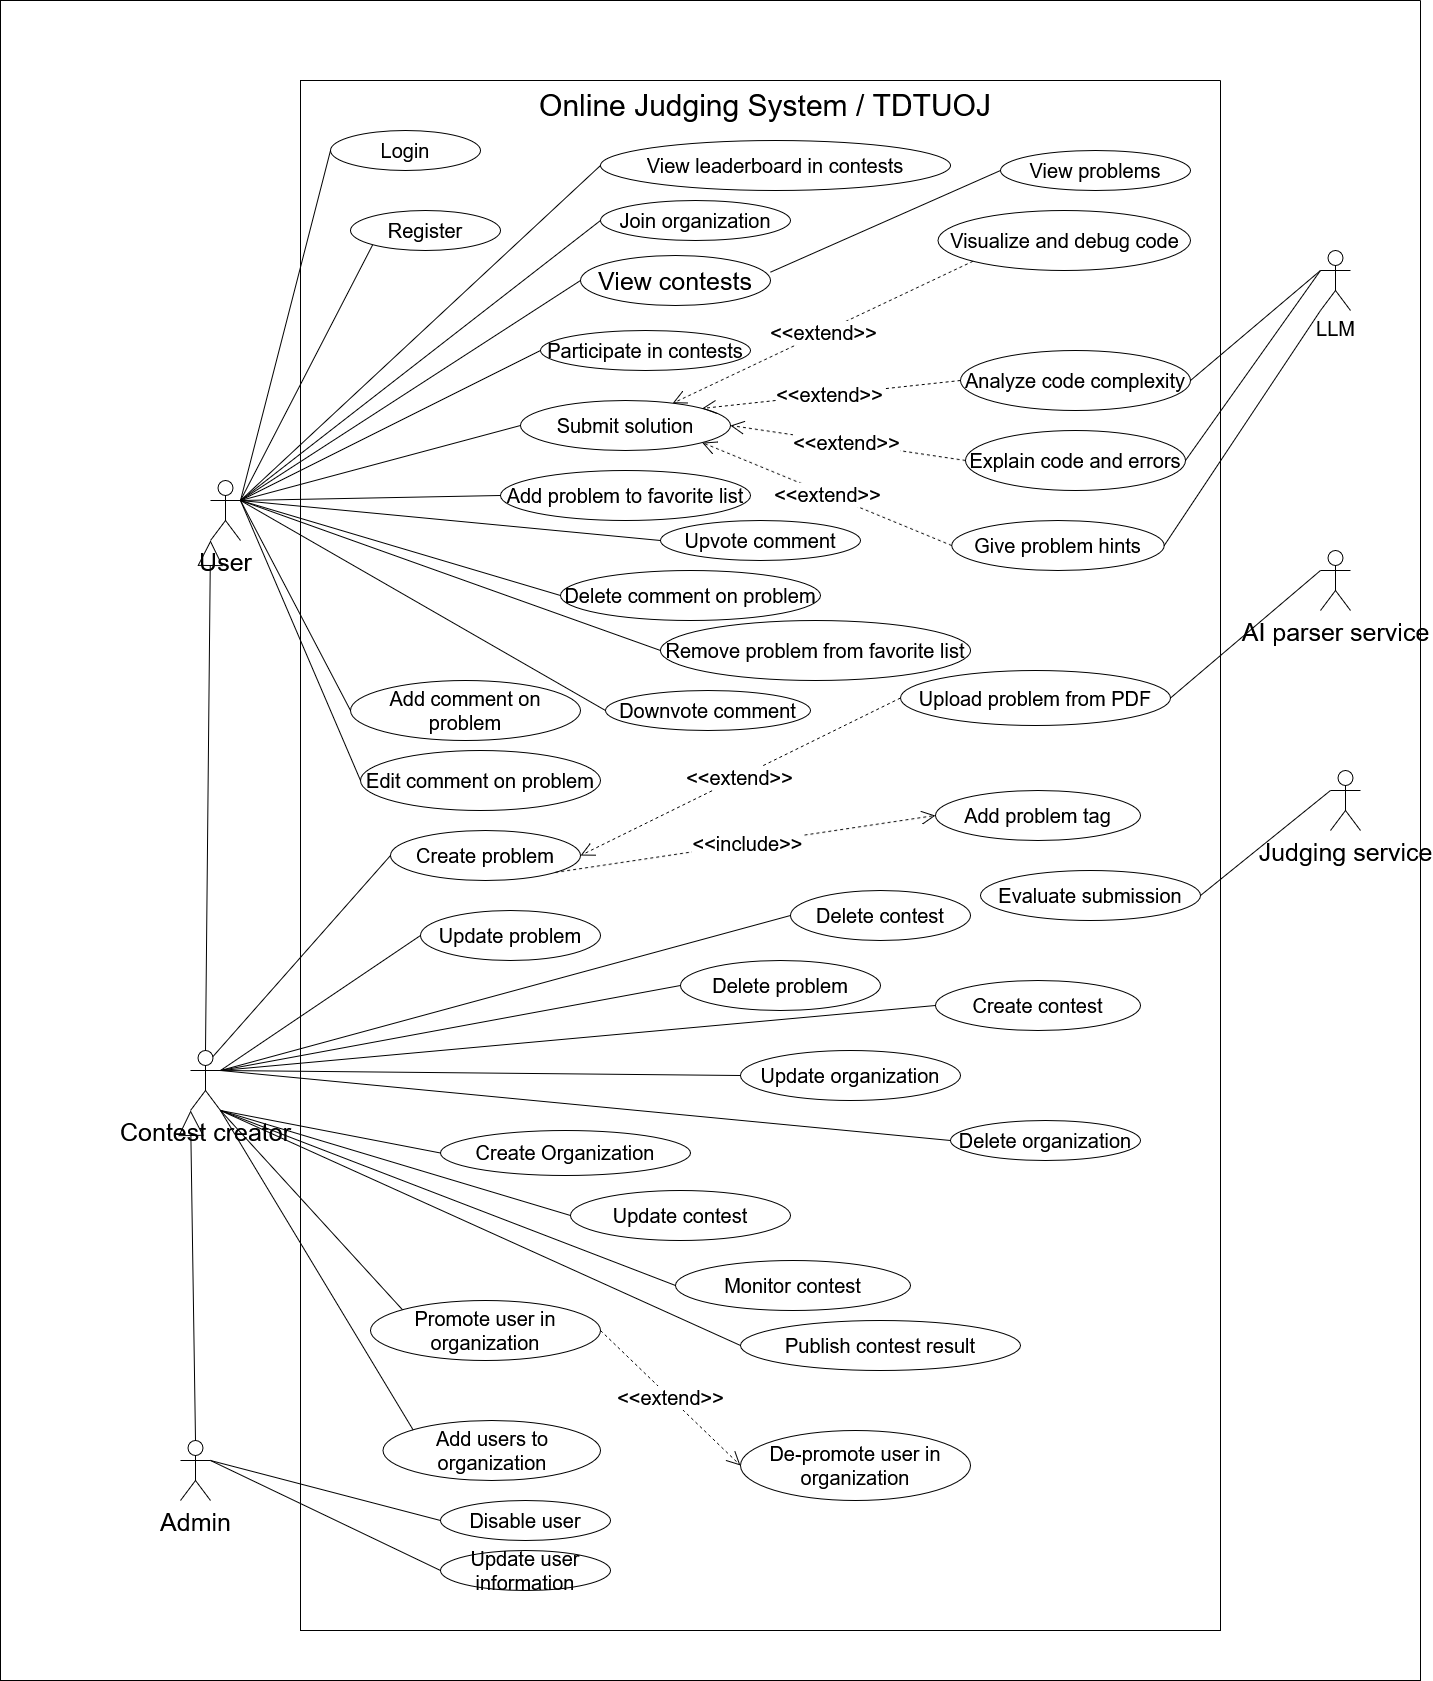
\includegraphics[width=0.92\textwidth]{figures/usecase.png}
  \caption{Sơ đồ Use Case tổng quan của hệ thống TDTUOJ}\label{fig:usecase}
\end{figure}

\subsection{Các Use Case chính}

% ── UC01: Nộp bài giải ───────────────────────────────────────
\subsubsection{Use case Nộp bài giải}

Nộp bài giải là Use Case trung tâm của hệ thống, phản ánh hoạt động cốt lõi của một nền
tảng chấm bài trực tuyến. Người dùng sau khi đọc đề bài sẽ viết lời giải trong trình soạn
thảo mã nguồn tích hợp, chọn ngôn ngữ lập trình phù hợp và gửi bài lên hệ thống để được
chấm tự động.

Sau khi tiếp nhận bài nộp, hệ thống lưu bản ghi với trạng thái chờ xử lý (PENDING), đưa bài
vào hàng đợi và chuyển đến dịch vụ chấm bài Judge0 để biên dịch và thực thi trên toàn bộ
test case. Kết quả chấm (verdict) cùng thời gian và bộ nhớ sử dụng được cập nhật và hiển thị
lại cho người dùng. Bảng~\ref{tab:uc01} trình bày đặc tả chi tiết của Use Case này.

\begin{longtable}{|>{\raggedright\arraybackslash\bfseries}p{2.8cm}|>{\raggedright\arraybackslash}p{5.7cm}|>{\raggedright\arraybackslash}p{5.7cm}|}
  \caption{Bảng đặc tả Use case Nộp bài giải}\label{tab:uc01} \\
  \hline
  \endfirsthead
  \hline
  \endhead
  \hline
  \endfoot
  \endlastfoot
  Use Case & \multicolumn{2}{p{11.9cm}|}{Nộp bài giải} \\
  \hline
  Bối cảnh & \multicolumn{2}{p{11.9cm}|}{Người dùng muốn kiểm tra tính đúng đắn và hiệu quả
    của lời giải mình viết cho một bài toán.} \\
  \hline
  Mô tả & \multicolumn{2}{p{11.9cm}|}{Người dùng gửi mã nguồn lời giải cho một bài toán bằng
    ngôn ngữ lập trình được chọn; hệ thống chấm bài tự động qua Judge0 và trả về kết quả.} \\
  \hline
  Tác nhân & \multicolumn{2}{p{11.9cm}|}{Người dùng (sinh viên).} \\
  \hline
  Sự kiện kích hoạt & \multicolumn{2}{p{11.9cm}|}{Người dùng nhấn nút ``Nộp bài'' trên trang
    chi tiết bài toán.} \\
  \hline
  Điều kiện tiên quyết & \multicolumn{2}{p{11.9cm}|}{+ Người dùng đã đăng nhập vào hệ
    thống.\newline + Bài toán đang công khai hoặc thuộc cuộc thi mà người dùng được phép
    truy cập.} \\
  \hline
  Kết quả & \multicolumn{2}{p{11.9cm}|}{Bài nộp được chấm tự động; kết quả chấm (\ac{AC},
    \ac{WA}, \ac{TLE}, \ac{MLE}, \ac{SF}, \ac{CE} hoặc \ac{IE}) được hiển thị và lưu lại để phục vụ
    thống kê và xếp hạng.} \\
  \hline
  Luồng sự kiện & \multicolumn{1}{c|}{\textbf{Tác nhân}}
                & \multicolumn{1}{c|}{\textbf{Hệ thống}} \\
  \cline{2-3}
   & 1. Người dùng viết lời giải trong trình soạn thảo và chọn ngôn ngữ lập trình. & \\
   & 2. Người dùng nhấn nút ``Nộp bài''.
     & 2.1 Hệ thống lưu bài nộp với trạng thái chờ xử lý (PENDING) và đưa vào hàng đợi
       Redis.\newline
       2.2 Hệ thống gửi mã nguồn cùng test case đến Judge0 để biên dịch và thực thi.\newline
       2.3 Hệ thống nhận kết quả chấm, cập nhật verdict, thời gian và bộ nhớ vào cơ sở dữ
       liệu. \\
   & 3. Người dùng xem kết quả bài nộp.
     & 3.1 Hệ thống hiển thị kết quả chấm (verdict) cùng thời gian và bộ nhớ cho người
       dùng. \\
  \hline
  Ngoại lệ & \multicolumn{2}{p{11.9cm}|}{Mã nguồn rỗng hoặc chưa chọn ngôn ngữ
    $\Rightarrow$ hệ thống hiển thị thông báo lỗi.\newline Bài nộp biên dịch lỗi
    $\Rightarrow$ hệ thống trả về kết quả \ac{CE} (Compilation Error).} \\
  \hline
\end{longtable}

Luồng xử lý của Use Case được mô tả trong sơ đồ hoạt động ở Hình~\ref{fig:act-uc01}.

\begin{figure}[H]
  \centering
  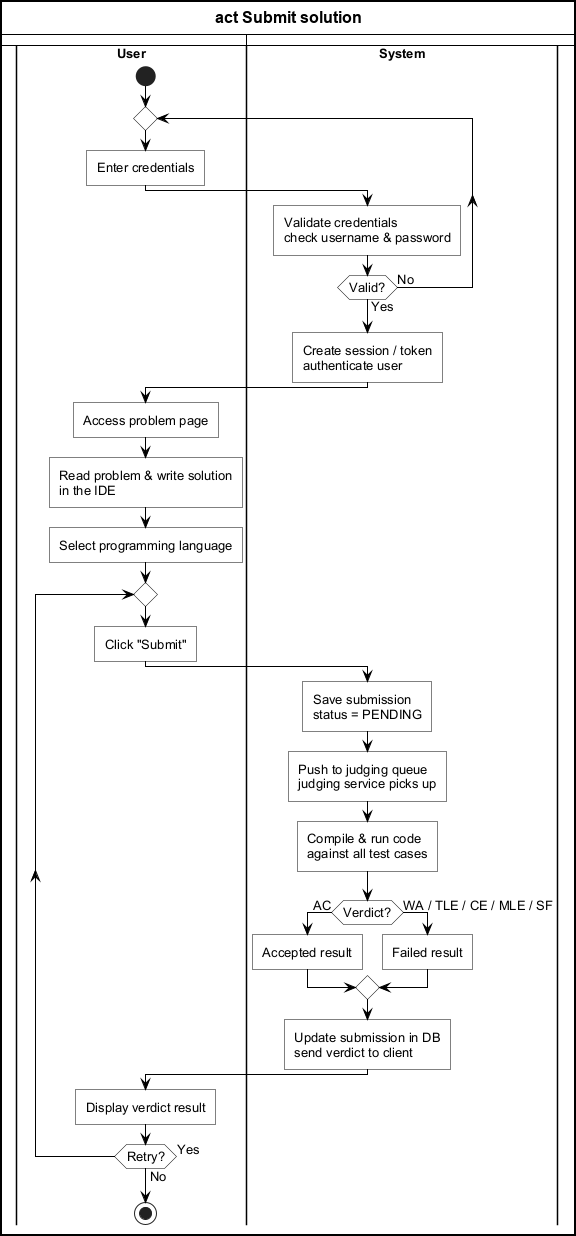
\includegraphics[width=0.70\textwidth,height=0.82\textheight,keepaspectratio]{figures/activity-submit.png}
  \caption{Sơ đồ hoạt động cho Use Case Nộp bài giải}\label{fig:act-uc01}
\end{figure}

Sự tương tác giữa người dùng và các thành phần của hệ thống được thể hiện qua sơ đồ tuần tự
trong Hình~\ref{fig:seq-uc01}.

\begin{figure}[H]
  \centering
  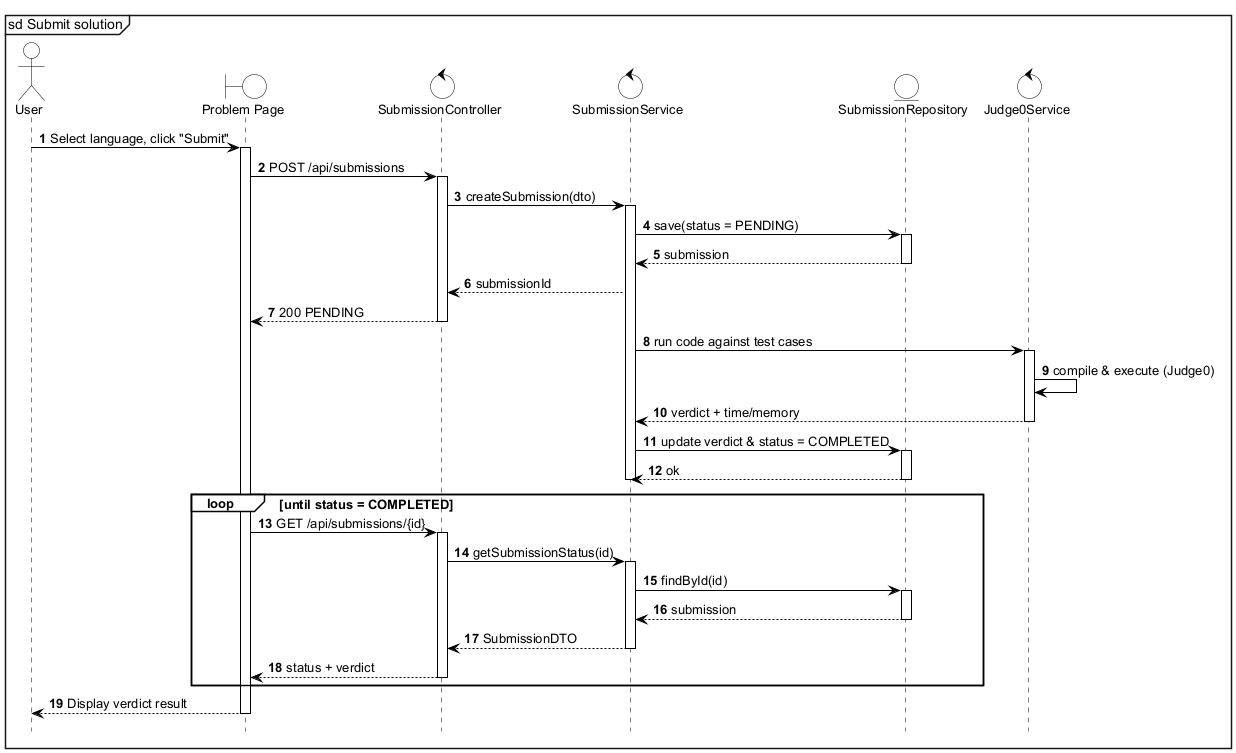
\includegraphics[width=\textwidth]{figures/seq-submit.png}
  \caption{Sơ đồ tuần tự cho Use Case Nộp bài giải}\label{fig:seq-uc01}
\end{figure}

% ── UC02: Tạo bài toán ───────────────────────────────────────
\subsubsection{Use case Tạo bài toán}

Tạo bài toán là Use Case cốt lõi của tác nhân Contest Creator, cho phép giảng viên xây dựng
kho đề phục vụ giảng dạy và tổ chức thi. Hệ thống hỗ trợ hai cách soạn đề: nhập thủ công
toàn bộ nội dung, hoặc tải lên tập tin \ac{PDF} để dịch vụ trích xuất bằng \ac{AI} (AI Parser)
tự động bóc tách đề bài và các test case mẫu, sau đó người tạo đề rà soát và chỉnh sửa lại.

Sau khi hoàn tất phần mô tả, người tạo đề gắn thẻ phân loại, thiết lập độ khó cùng phạm
vi hiển thị, rồi bổ sung các trường hợp kiểm thử (test case) bằng cách nhập tay hoặc nhờ
\ac{AI} sinh tự động. Khi lưu, hệ thống kiểm tra tính hợp lệ, sinh đường dẫn rút gọn (slug)
và lưu bài toán cùng toàn bộ test case vào cơ sở dữ liệu. Bảng~\ref{tab:uc02} trình bày đặc
tả chi tiết của Use Case này.

\begin{longtable}{|>{\raggedright\arraybackslash\bfseries}p{2.8cm}|>{\raggedright\arraybackslash}p{5.7cm}|>{\raggedright\arraybackslash}p{5.7cm}|}
  \caption{Bảng đặc tả Use case Tạo bài toán}\label{tab:uc02} \\
  \hline
  \endfirsthead
  \hline
  \endhead
  \hline
  \endfoot
  \endlastfoot
  Use Case & \multicolumn{2}{p{11.9cm}|}{Tạo bài toán} \\
  \hline
  Bối cảnh & \multicolumn{2}{p{11.9cm}|}{Giảng viên muốn bổ sung một bài toán mới vào kho đề
    để giao bài thực hành hoặc tổ chức cuộc thi.} \\
  \hline
  Mô tả & \multicolumn{2}{p{11.9cm}|}{Người tạo đề soạn nội dung bài toán (thủ công hoặc
    trích xuất từ \ac{PDF}), gắn thẻ, thiết lập cấu hình và thêm test case; hệ thống kiểm tra
    và lưu bài toán.} \\
  \hline
  Tác nhân & \multicolumn{2}{p{11.9cm}|}{Contest Creator (giảng viên), Admin.} \\
  \hline
  Sự kiện kích hoạt & \multicolumn{2}{p{11.9cm}|}{Người tạo đề mở biểu mẫu ``Tạo bài toán''.} \\
  \hline
  Điều kiện tiên quyết & \multicolumn{2}{p{11.9cm}|}{+ Người dùng đã đăng nhập với vai trò
    Contest Creator hoặc Admin.} \\
  \hline
  Kết quả & \multicolumn{2}{p{11.9cm}|}{Bài toán mới được lưu cùng các test case; hệ thống
    sinh slug và hiển thị trang chi tiết bài toán vừa tạo.} \\
  \hline
  Luồng sự kiện & \multicolumn{1}{c|}{\textbf{Tác nhân}}
                & \multicolumn{1}{c|}{\textbf{Hệ thống}} \\
  \cline{2-3}
   & 1. Người tạo đề mở biểu mẫu ``Tạo bài toán'' và chọn cách soạn (thủ công hoặc nhập từ
     \ac{PDF}). & \\
   & 2. (Tùy chọn) Người tạo đề tải lên tập tin \ac{PDF}.
     & 2.1 Hệ thống gửi tập tin đến dịch vụ \ac{AI} để trích xuất đề bài và ví dụ mẫu.\newline
       2.2 Hệ thống điền sẵn các trường thông tin và trả về cho người tạo đề rà soát. \\
   & 3. Người tạo đề chỉnh sửa nội dung, gắn thẻ, thiết lập mức độ khó và phạm vi hiển thị. & \\
   & 4. Người tạo đề thêm test case bằng cách nhập tay hoặc yêu cầu \ac{AI} sinh tự động, và
     đánh dấu test case là test case mẫu hay ẩn.
     & 4.1 Khi được yêu cầu, hệ thống gọi dịch vụ \ac{AI} sinh các test case và trả về cho
       người tạo đề. \\
   & 5. Người tạo đề nhấn nút ``Lưu bài toán''.
     & 5.1 Hệ thống kiểm tra tính hợp lệ của các trường thông tin và test case.\newline
       5.2 Hệ thống sinh slug, lưu bài toán cùng test case vào cơ sở dữ liệu và trả về bài
       toán đã tạo. \\
   & 6. Người tạo đề xem trang chi tiết bài toán. & 6.1 Hệ thống hiển thị trang bài toán vừa
     được tạo. \\
  \hline
  Ngoại lệ & \multicolumn{2}{p{11.9cm}|}{Thiếu trường bắt buộc hoặc chưa có test case hợp lệ
    $\Rightarrow$ hệ thống hiển thị thông báo lỗi và không lưu bài toán.} \\
  \hline
\end{longtable}

Luồng xử lý của Use Case được mô tả trong sơ đồ hoạt động ở Hình~\ref{fig:act-uc02}.

\begin{figure}[H]
  \centering
  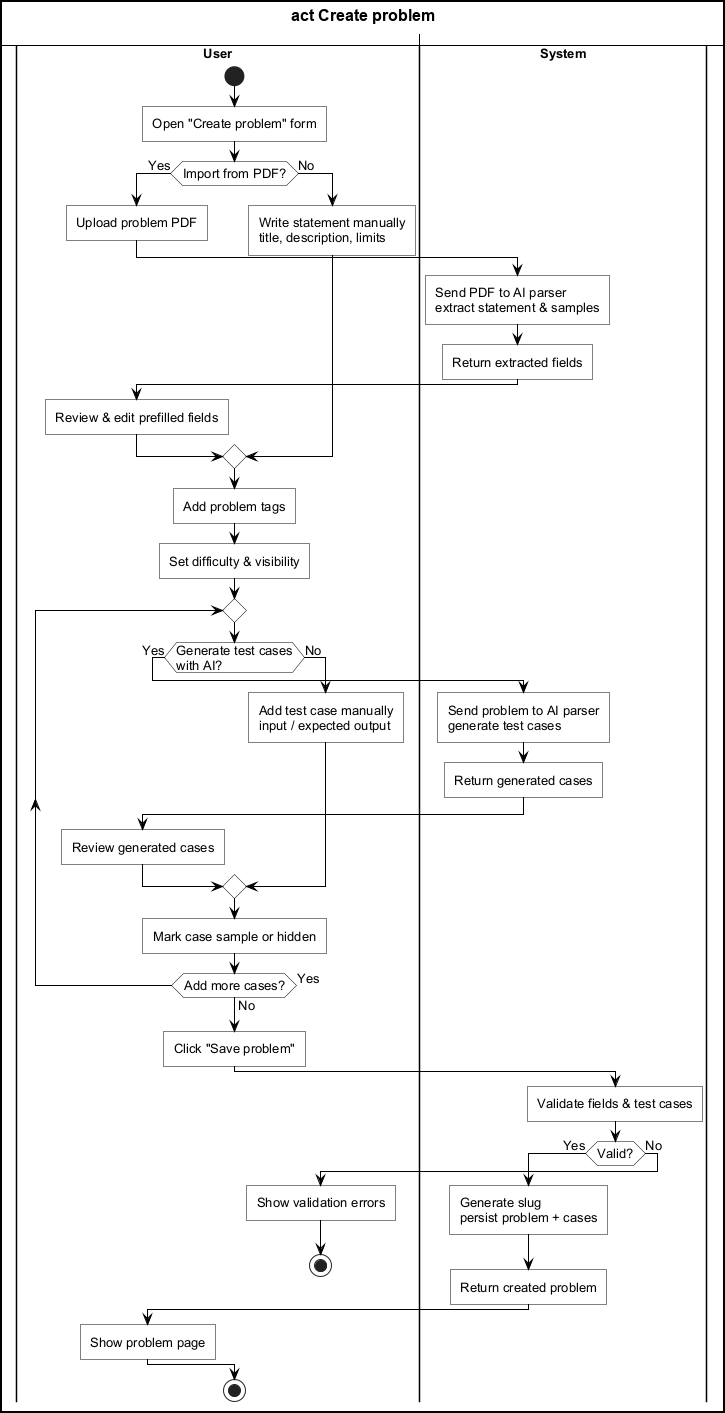
\includegraphics[width=0.70\textwidth,height=0.82\textheight,keepaspectratio]{figures/activity-create-problem.png}
  \caption{Sơ đồ hoạt động cho Use Case Tạo bài toán}\label{fig:act-uc02}
\end{figure}

Sự tương tác giữa người tạo đề và các thành phần của hệ thống được thể hiện qua sơ đồ tuần tự
trong Hình~\ref{fig:seq-uc02}.

\begin{figure}[H]
  \centering
  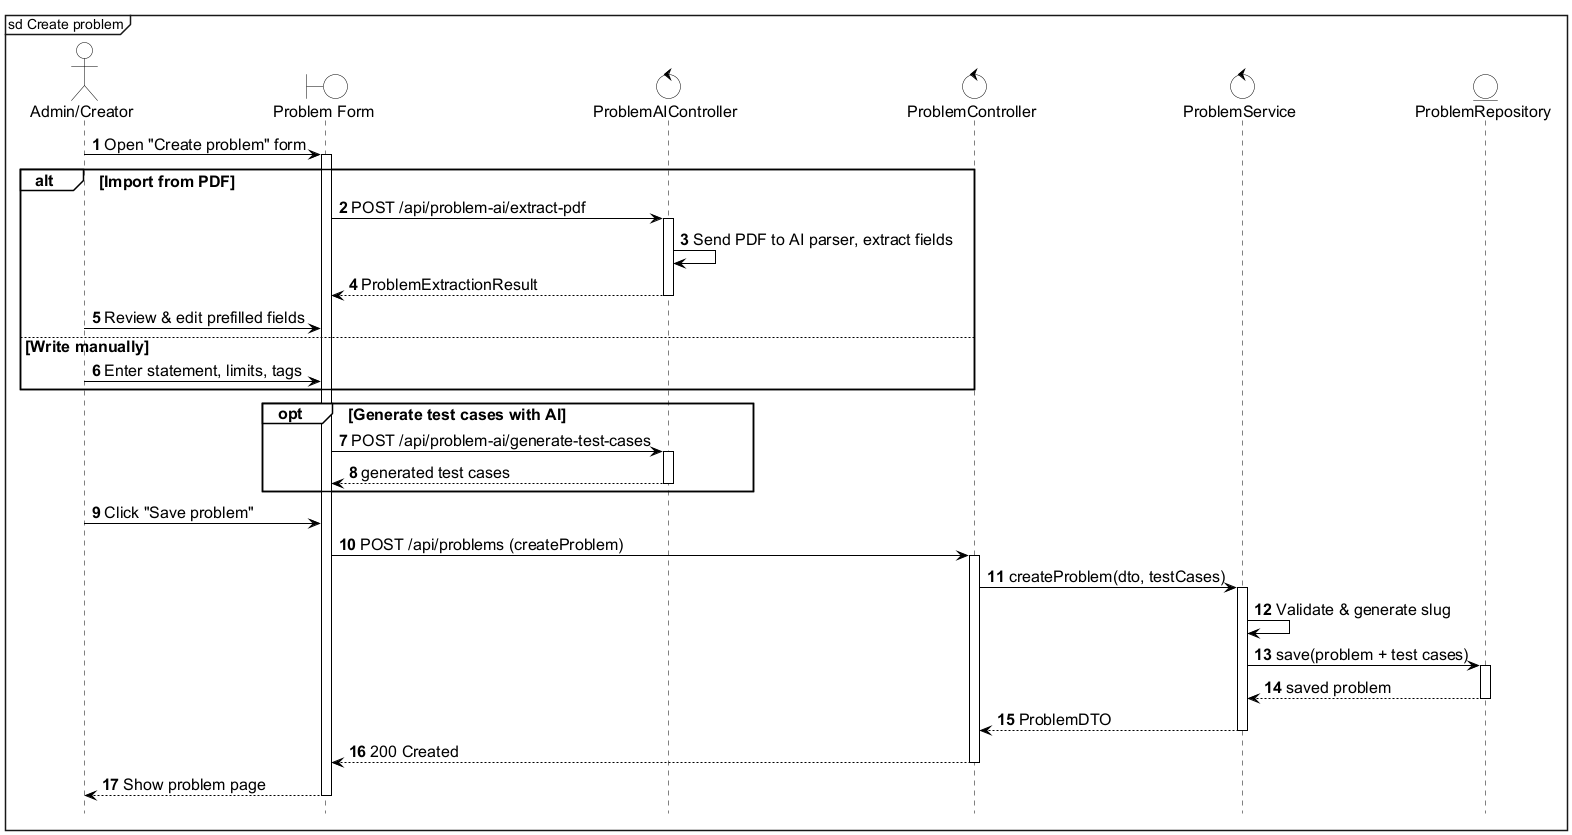
\includegraphics[width=\textwidth]{figures/seq-create-problem.png}
  \caption{Sơ đồ tuần tự cho Use Case Tạo bài toán}\label{fig:seq-uc02}
\end{figure}

% ── UC03: Trực quan hóa và gỡ lỗi mã nguồn ──────────────────
\subsubsection{Use case Trực quan hóa và gỡ lỗi mã nguồn}

Trực quan hóa và gỡ lỗi mã nguồn là Use Case đặc trưng của hệ thống, hỗ trợ người học hiểu
cách lời giải vận hành thay vì chỉ nhận về kết quả đúng hay sai. Người dùng viết mã nguồn,
chọn ngôn ngữ lập trình, sau đó yêu cầu hệ thống minh họa quá trình thực thi.

Hệ thống chọn bộ ghi vết (tracer) tương ứng với ngôn ngữ để biến đổi mã nguồn sao cho khi
chạy, chương trình tự phát ra chuỗi khung trạng thái (frame) mô tả callstack và các
biến tại từng dòng lệnh, rồi gửi mã đã biến đổi đến dịch vụ chấm bài để thực thi trong môi
trường cô lập. Vết thực thi được phân tích thành chuỗi các bước; giao diện hiển thị từng bước dưới dạng
mảng, cây, đồ thị hoặc cấu trúc tương ứng để người dùng theo dõi. Bảng~\ref{tab:uc03} trình
bày đặc tả chi tiết của Use Case này.

\begin{longtable}{|>{\raggedright\arraybackslash\bfseries}p{2.8cm}|>{\raggedright\arraybackslash}p{5.7cm}|>{\raggedright\arraybackslash}p{5.7cm}|}
  \caption{Bảng đặc tả Use case Trực quan hóa và gỡ lỗi mã nguồn}\label{tab:uc03} \\
  \hline
  \endfirsthead
  \hline
  \endhead
  \hline
  \endfoot
  \endlastfoot
  Use Case & \multicolumn{2}{p{11.9cm}|}{Trực quan hóa và gỡ lỗi mã nguồn} \\
  \hline
  Bối cảnh & \multicolumn{2}{p{11.9cm}|}{Người dùng muốn quan sát trạng thái các biến và cấu
    trúc dữ liệu qua từng bước để hiểu hoặc gỡ lỗi lời giải.} \\
  \hline
  Mô tả & \multicolumn{2}{p{11.9cm}|}{Hệ thống biến đổi mã nguồn để tự ghi vết khi chạy,
    thực thi qua dịch vụ chấm bài và phân tích vết thành các bước minh họa cho người dùng
    xem lại.} \\
  \hline
  Tác nhân & \multicolumn{2}{p{11.9cm}|}{Người dùng (sinh viên).} \\
  \hline
  Sự kiện kích hoạt & \multicolumn{2}{p{11.9cm}|}{Người dùng nhấn nút ``Trực quan hóa''
    (Visualize) trong trình soạn thảo.} \\
  \hline
  Điều kiện tiên quyết & \multicolumn{2}{p{11.9cm}|}{+ Người dùng đã viết mã nguồn và chọn
    ngôn ngữ lập trình được hỗ trợ (Python, JavaScript, Java, C\#, C, C++).} \\
  \hline
  Kết quả & \multicolumn{2}{p{11.9cm}|}{Quá trình thực thi được minh họa theo từng bước; người
    dùng có thể duyệt tới lui hoặc phát hoạt ảnh để quan sát trạng thái dữ liệu.} \\
  \hline
  Luồng sự kiện & \multicolumn{1}{c|}{\textbf{Tác nhân}}
                & \multicolumn{1}{c|}{\textbf{Hệ thống}} \\
  \cline{2-3}
   & 1. Người dùng viết mã nguồn và chọn ngôn ngữ lập trình. & \\
   & 2. Người dùng nhấn nút ``Trực quan hóa''.
     & 2.1 Hệ thống chọn bộ ghi vết theo ngôn ngữ và biến đổi mã nguồn để tự phát ra khung
       trạng thái khi chạy.\newline
       2.2 Hệ thống gửi mã đã biến đổi đến dịch vụ chấm bài để biên dịch và thực thi, thu lại
       vết thực thi; song song, mô hình ngôn ngữ lớn phân loại vai trò của các biến.\newline
       2.3 Hệ thống phân tích vết thực thi thành chuỗi các bước kèm snapshot trạng thái biến
       và trả về danh sách bước cùng kết quả phân loại. \\
   & 3. Người dùng duyệt từng bước, bước tới lui hoặc phát hoạt ảnh trong trình minh họa.
     & 3.1 Hệ thống hiển thị trạng thái dữ liệu tại mỗi bước bằng trình minh họa phù hợp. \\
  \hline
  Ngoại lệ & \multicolumn{2}{p{11.9cm}|}{Mã nguồn biên dịch lỗi hoặc gặp lỗi khi chạy
    $\Rightarrow$ hệ thống trả về thông báo lỗi để người dùng sửa lại mã nguồn.} \\
  \hline
\end{longtable}

Luồng xử lý của Use Case được mô tả trong sơ đồ hoạt động ở Hình~\ref{fig:act-uc03}.

\begin{figure}[H]
  \centering
  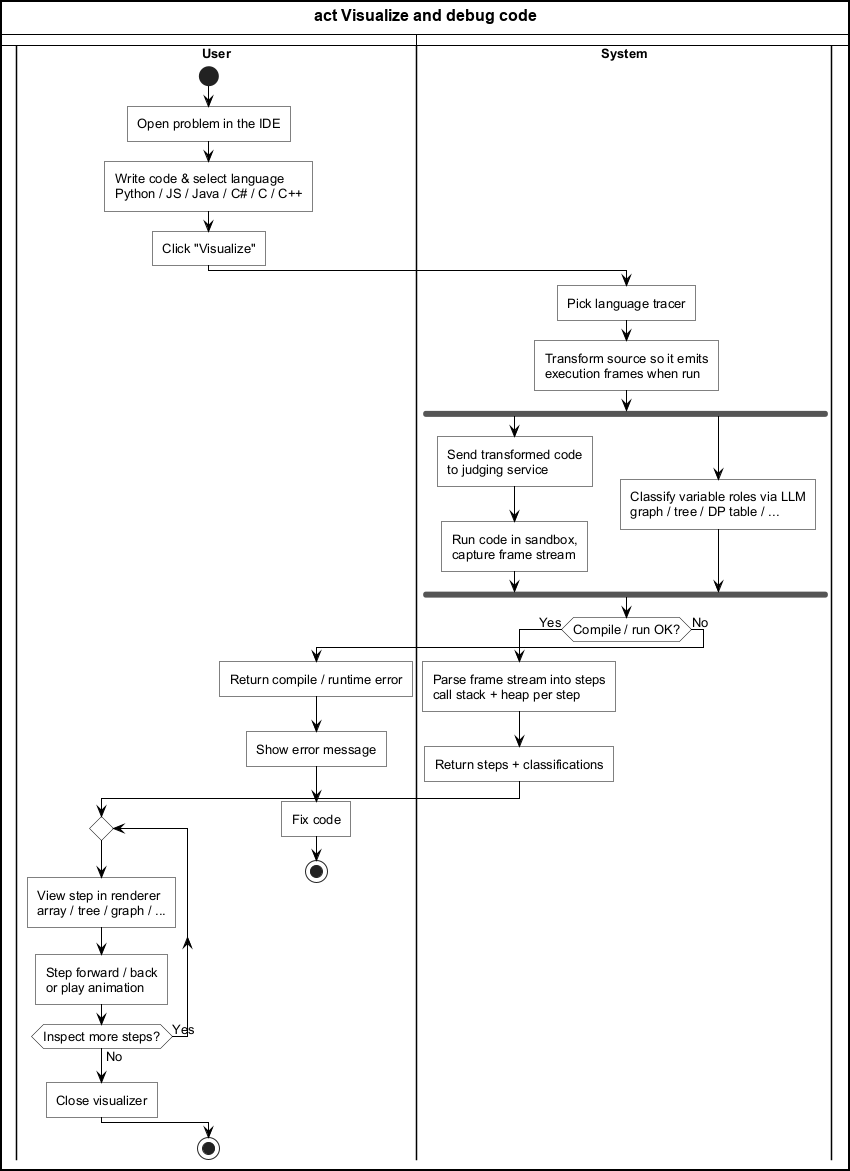
\includegraphics[width=0.70\textwidth,height=0.82\textheight,keepaspectratio]{figures/activity-visualize.png}
  \caption{Sơ đồ hoạt động cho Use Case Trực quan hóa và gỡ lỗi mã nguồn}\label{fig:act-uc03}
\end{figure}

Sự tương tác giữa người dùng và các thành phần của hệ thống được thể hiện qua sơ đồ tuần tự
trong Hình~\ref{fig:seq-uc03}.

\begin{figure}[H]
  \centering
  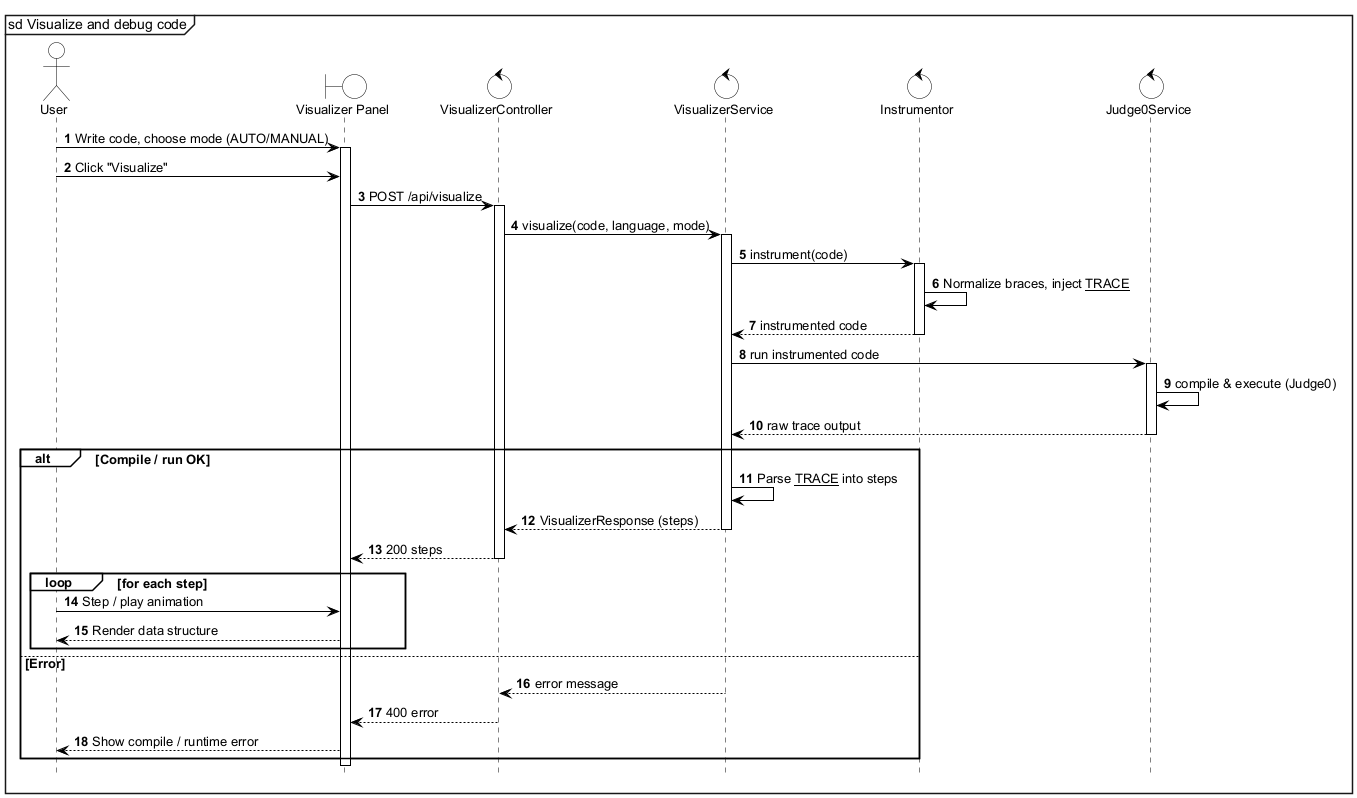
\includegraphics[width=\textwidth]{figures/seq-visualize.png}
  \caption{Sơ đồ tuần tự cho Use Case Trực quan hóa và gỡ lỗi mã nguồn}\label{fig:seq-uc03}
\end{figure}

% ── UC04: Tham gia cuộc thi ──────────────────────────────────
\subsubsection{Use case Tham gia cuộc thi}

Tham gia cuộc thi cho phép người dùng thi đấu trực tuyến trên hệ thống theo thể thức \ac{ICPC}.
Người dùng đăng ký tham gia một cuộc thi và được xác nhận tham gia ngay, miễn
là cuộc thi còn trong thời gian cho phép đăng ký và chưa đạt giới hạn số lượng người tham gia.

Trong thời gian diễn ra, người dùng mở từng bài toán, viết lời giải và nộp bài; hệ thống chấm
bài, tính điểm theo thể thức và cập nhật bảng xếp hạng theo thời gian thực để người dùng theo
dõi thứ hạng. Nhằm bảo đảm tính công bằng, bài nộp trong cuộc thi được ẩn khỏi những người
dùng khác cho đến khi cuộc thi kết thúc; nếu người tạo cuộc thi cấu hình khoảng đóng băng,
bảng xếp hạng công khai ngừng cập nhật trong những phút cuối theo thể thức \ac{ICPC}. Khi
cuộc thi kết thúc, hệ thống tự động tính toán và cập nhật lịch sử điểm xếp hạng (rating),
mở lại quyền xem bài nộp và công khai các bài toán của cuộc thi vào kho luyện tập.
Bảng~\ref{tab:uc04} trình bày đặc tả chi tiết của Use Case này.

\begin{longtable}{|>{\raggedright\arraybackslash\bfseries}p{2.8cm}|>{\raggedright\arraybackslash}p{5.7cm}|>{\raggedright\arraybackslash}p{5.7cm}|}
  \caption{Bảng đặc tả Use case Tham gia cuộc thi}\label{tab:uc04} \\
  \hline
  \endfirsthead
  \hline
  \endhead
  \hline
  \endfoot
  \endlastfoot
  Use Case & \multicolumn{2}{p{11.9cm}|}{Tham gia cuộc thi} \\
  \hline
  Bối cảnh & \multicolumn{2}{p{11.9cm}|}{Người dùng muốn thi đấu trong một cuộc thi lập trình
    được tổ chức trên hệ thống.} \\
  \hline
  Mô tả & \multicolumn{2}{p{11.9cm}|}{Người dùng đăng ký, nộp bài trong thời gian thi và theo
    dõi bảng xếp hạng; hệ thống chấm bài, tính điểm theo thể thức và cập nhật rating khi kết
    thúc.} \\
  \hline
  Tác nhân & \multicolumn{2}{p{11.9cm}|}{Người dùng (sinh viên); Contest Creator (tổ chức và
    công bố kết quả).} \\
  \hline
  Sự kiện kích hoạt & \multicolumn{2}{p{11.9cm}|}{Người dùng nhấn nút ``Đăng ký'' trên trang
    chi tiết cuộc thi.} \\
  \hline
  Điều kiện tiên quyết & \multicolumn{2}{p{11.9cm}|}{+ Người dùng đã đăng nhập.\newline + Cuộc
    thi đang ở trạng thái cho phép đăng ký.} \\
  \hline
  Kết quả & \multicolumn{2}{p{11.9cm}|}{Người dùng được ghi nhận tham gia; điểm và thứ hạng
    được tính, bảng xếp hạng cuối cùng cùng rating được cập nhật.} \\
  \hline
  Luồng sự kiện & \multicolumn{1}{c|}{\textbf{Tác nhân}}
                & \multicolumn{1}{c|}{\textbf{Hệ thống}} \\
  \cline{2-3}
   & 1. Người dùng mở trang cuộc thi và nhấn nút ``Đăng ký''.
     & 1.1 Hệ thống kiểm tra điều kiện đăng ký (còn thời hạn, chưa đầy chỗ, chưa đăng ký) rồi
       tạo bản ghi đăng ký với trạng thái APPROVED và xác nhận tham gia ngay. \\
   & 2. Người dùng chờ đến giờ thi, mở bài toán và nộp lời giải.
     & 2.1 Hệ thống chấm bài nộp và tính điểm theo thể thức \ac{ICPC}.\newline
       2.2 Hệ thống ẩn bài nộp khỏi những người dùng khác cho đến khi cuộc thi kết
       thúc.\newline
       2.3 Hệ thống cập nhật bảng xếp hạng theo thời gian thực; trong khoảng đóng băng,
       người xem thông thường nhận snapshot bảng xếp hạng tại thời điểm đóng băng. \\
   & 3. Người dùng xem kết quả chấm và thứ hạng trực tiếp. & 3.1 Hệ thống hiển thị kết quả
     chấm cùng thứ hạng hiện thời. \\
   & 4. Người dùng xem kết quả chung cuộc.
     & 4.1 Khi cuộc thi kết thúc, hệ thống tự động tính toán điểm xếp hạng và cập nhật lịch
       sử rating.\newline
       4.2 Hệ thống mở lại quyền xem bài nộp, công khai các bài toán của cuộc thi và hiển
       thị bảng xếp hạng cuối cùng. \\
  \hline
  Ngoại lệ & \multicolumn{2}{p{11.9cm}|}{Cuộc thi đã kết thúc, đã đạt giới hạn số người tham
    gia, hoặc người dùng đã đăng ký trước đó $\Rightarrow$ hệ thống từ chối và thông báo lý do.} \\
  \hline
\end{longtable}

Luồng xử lý của Use Case được mô tả trong sơ đồ hoạt động ở Hình~\ref{fig:act-uc04}.

\begin{figure}[H]
  \centering
  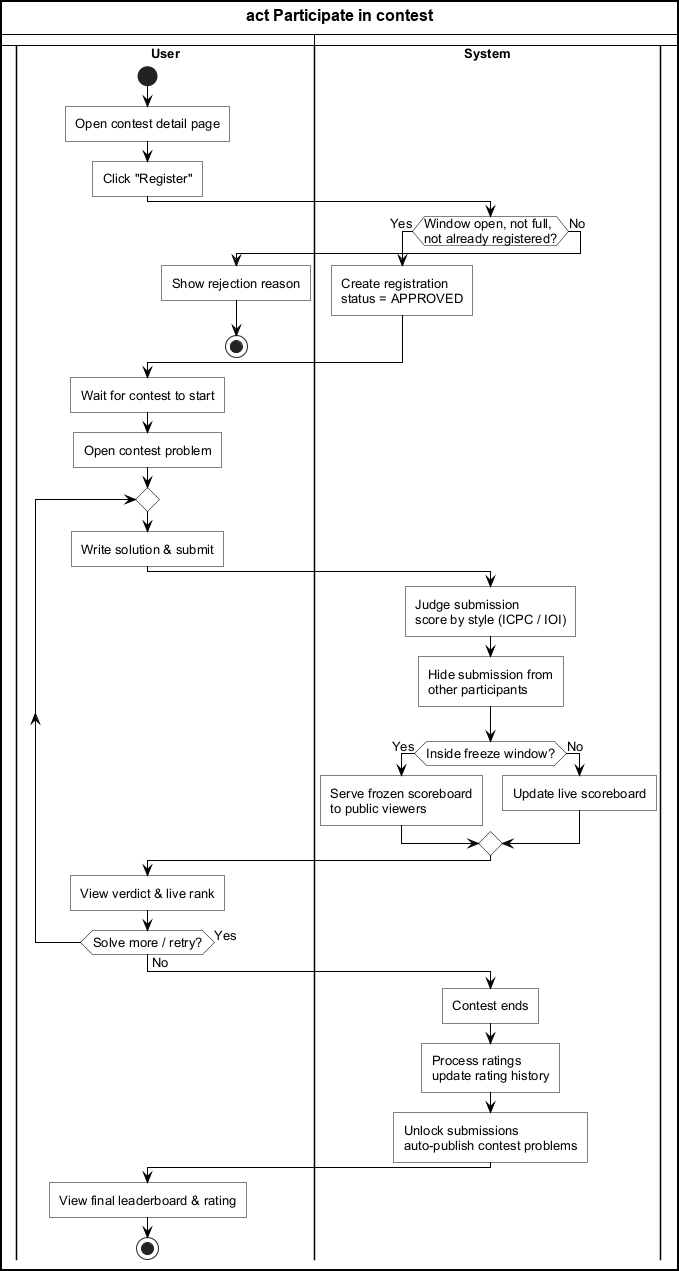
\includegraphics[width=0.70\textwidth,height=0.82\textheight,keepaspectratio]{figures/activity-participate-contest.png}
  \caption{Sơ đồ hoạt động cho Use Case Tham gia cuộc thi}\label{fig:act-uc04}
\end{figure}

Sự tương tác giữa người dùng và các thành phần của hệ thống được thể hiện qua sơ đồ tuần tự
trong Hình~\ref{fig:seq-uc04}.

\begin{figure}[H]
  \centering
  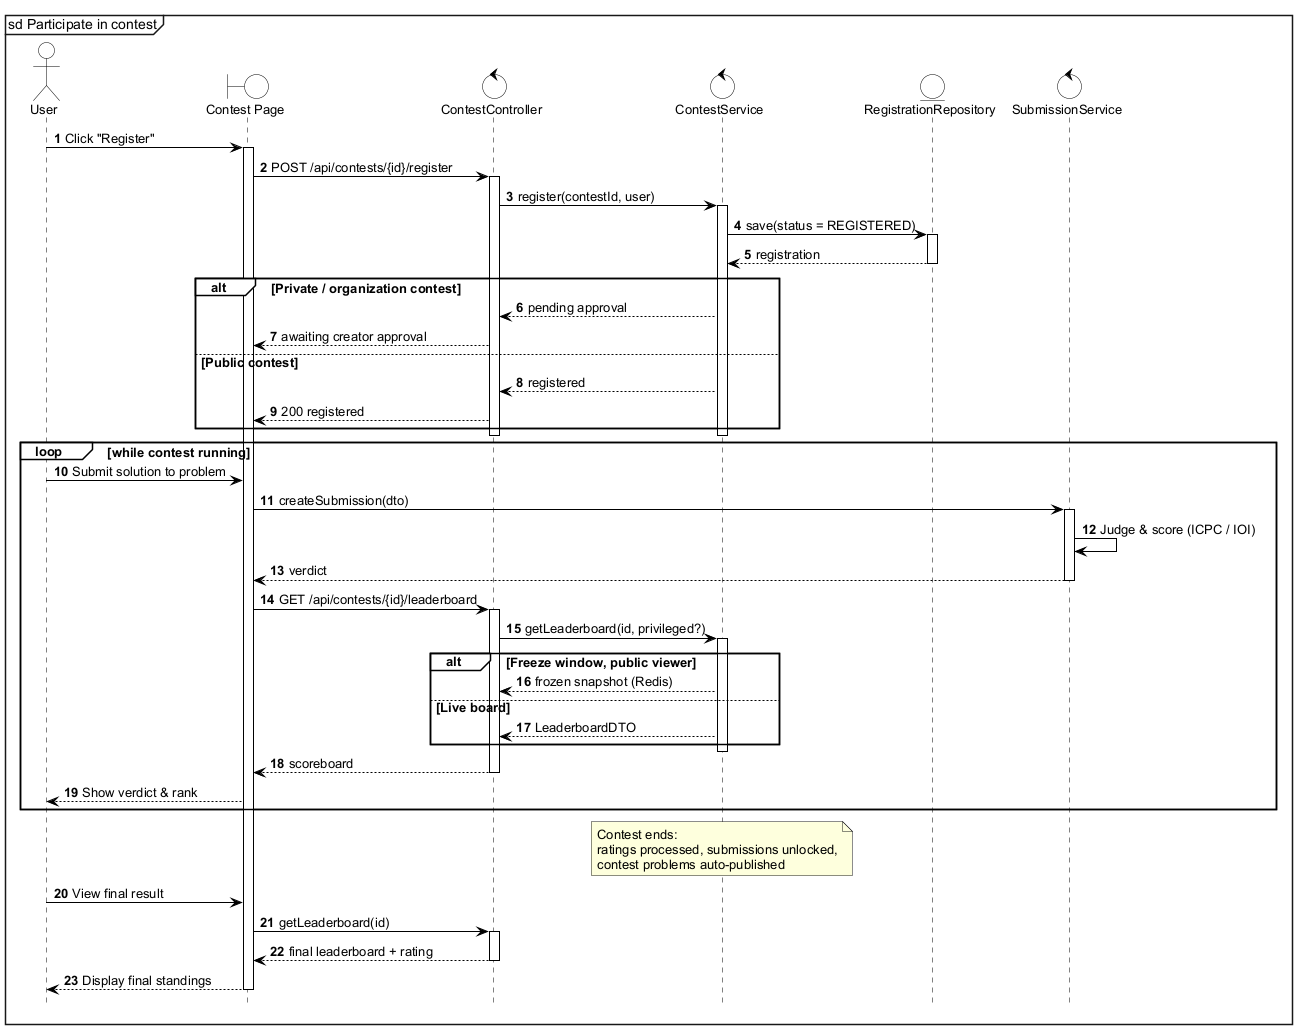
\includegraphics[width=\textwidth]{figures/seq-participate-contest.png}
  \caption{Sơ đồ tuần tự cho Use Case Tham gia cuộc thi}\label{fig:seq-uc04}
\end{figure}

% ── UC05: Gợi ý học tập bằng LLM ─────────────────────────────
\subsubsection{Use case Gợi ý học tập bằng LLM}

Gợi ý học tập bằng \ac{LLM} hỗ trợ người dùng giải thích các vướng mắc trong quá trình luyện tập mà không tiết lộ lời
giải hoàn chỉnh. Người dùng mở khung gợi ý trong trang bài toán, nhập câu hỏi hoặc chọn một mẫu yêu cầu sẵn có như gợi ý hướng
tiếp cận, giải thích đề bài hay phân tích độ phức tạp.

Hệ thống xác định dịch vụ mô hình tương ứng, dựng câu nhắc (prompt) được kiểm soát chỉ chứa
ngữ cảnh của bài toán hiện tại, rồi gọi đến API \ac{LLM}. Nếu câu hỏi đúng phạm vi bài
toán, hệ thống trả về gợi ý mà không kèm thêm lời giải đầy đủ; ngược lại, hệ thống trả về thông báo từ
chối nhằm ngăn lạm dụng API. Bảng~\ref{tab:uc05} trình bày đặc tả chi tiết của Use Case này.

\begin{longtable}{|>{\raggedright\arraybackslash\bfseries}p{2.8cm}|>{\raggedright\arraybackslash}p{5.7cm}|>{\raggedright\arraybackslash}p{5.7cm}|}
  \caption{Bảng đặc tả Use case Gợi ý học tập bằng \ac{LLM}}\label{tab:uc05} \\
  \hline
  \endfirsthead
  \hline
  \endhead
  \hline
  \endfoot
  \endlastfoot
  Use Case & \multicolumn{2}{p{11.9cm}|}{Gợi ý học tập bằng \ac{LLM}} \\
  \hline
  Bối cảnh & \multicolumn{2}{p{11.9cm}|}{Người dùng gặp khó khăn với một bài toán và muốn nhận
    gợi ý định hướng thay vì lời giải hoàn chỉnh.} \\
  \hline
  Mô tả & \multicolumn{2}{p{11.9cm}|}{Người dùng đặt câu hỏi cho mô hình ngôn ngữ lớn về bài
    toán; hệ thống dựng câu nhắc có kiểm soát và trả về gợi ý đúng phạm vi, không tiết lộ lời
    giải đầy đủ.} \\
  \hline
  Tác nhân & \multicolumn{2}{p{11.9cm}|}{Người dùng (sinh viên); hệ thống \ac{LLM} bên
    ngoài.} \\
  \hline
  Sự kiện kích hoạt & \multicolumn{2}{p{11.9cm}|}{Người dùng gửi câu hỏi trong khung gợi ý của
    trang bài toán.} \\
  \hline
  Điều kiện tiên quyết & \multicolumn{2}{p{11.9cm}|}{+ Người dùng đã đăng nhập và đang xem một
    bài toán cụ thể.} \\
  \hline
  Kết quả & \multicolumn{2}{p{11.9cm}|}{Người dùng nhận gợi ý phù hợp với bài toán; các câu hỏi
    ngoài phạm vi bị từ chối.} \\
  \hline
  Luồng sự kiện & \multicolumn{1}{c|}{\textbf{Tác nhân}}
                & \multicolumn{1}{c|}{\textbf{Hệ thống}} \\
  \cline{2-3}
   & 1. Người dùng mở khung gợi ý và chọn mô hình ngôn ngữ lớn. & \\
   & 2. Người dùng nhập câu hỏi hoặc chọn một mẫu yêu cầu sẵn có.
     & 2.1 Hệ thống xác định dịch vụ mô hình tương ứng và dựng câu nhắc có kiểm soát, chỉ chứa
       ngữ cảnh bài toán.\newline
       2.2 Hệ thống gọi nhà cung cấp \ac{LLM} và nhận phản hồi.\newline
       2.3 Nếu câu hỏi đúng phạm vi, hệ thống trả về gợi ý không kèm lời giải đầy đủ; nếu
       không, hệ thống trả về thông báo từ chối. \\
   & 3. Người dùng đọc gợi ý và có thể đặt câu hỏi tiếp theo. & 3.1 Hệ thống hiển thị phản hồi
     trong khung gợi ý. \\
  \hline
  Ngoại lệ & \multicolumn{2}{p{11.9cm}|}{Câu hỏi nằm ngoài phạm vi bài toán $\Rightarrow$ hệ
    thống trả về thông báo từ chối và không sinh gợi ý.} \\
  \hline
\end{longtable}

Luồng xử lý của Use Case được mô tả trong sơ đồ hoạt động ở Hình~\ref{fig:act-uc05}.

\begin{figure}[H]
  \centering
  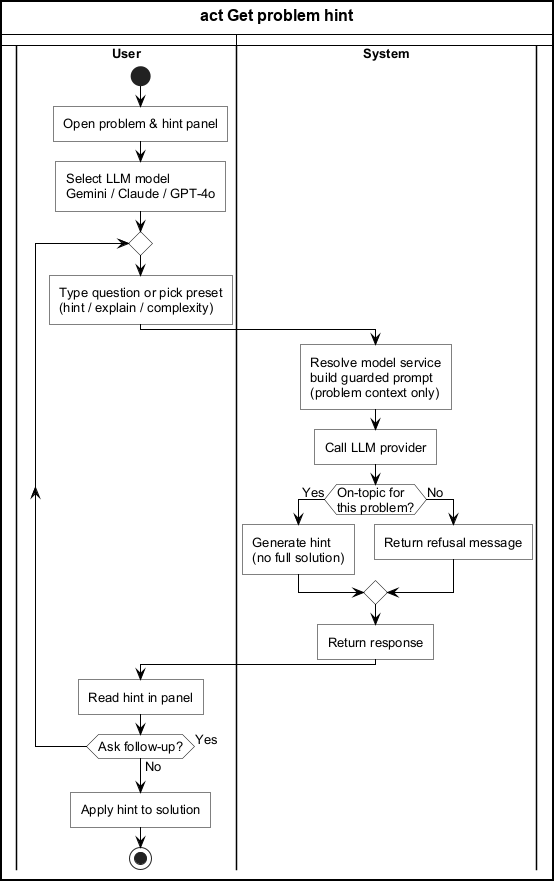
\includegraphics[width=0.70\textwidth,height=0.82\textheight,keepaspectratio]{figures/activity-hint.png}
  \caption{Sơ đồ hoạt động cho Use Case Gợi ý học tập bằng \ac{LLM}}\label{fig:act-uc05}
\end{figure}

Sự tương tác giữa người dùng và các thành phần của hệ thống được thể hiện qua sơ đồ tuần tự
trong Hình~\ref{fig:seq-uc05}.

\begin{figure}[H]
  \centering
  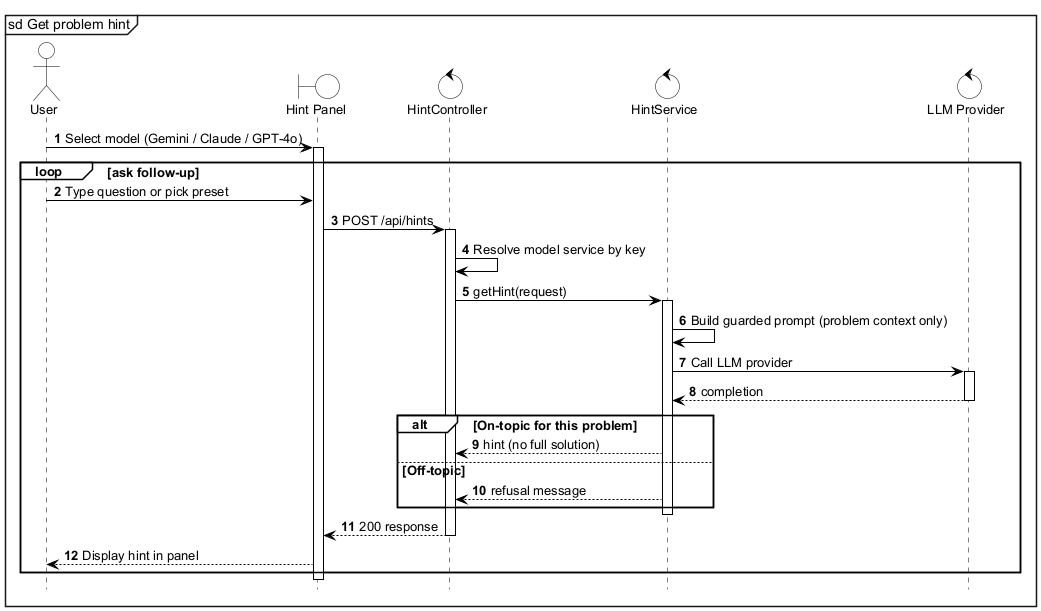
\includegraphics[width=\textwidth]{figures/seq-hint.png}
  \caption{Sơ đồ tuần tự cho Use Case Gợi ý học tập bằng \ac{LLM}}\label{fig:seq-uc05}
\end{figure}

% ── UC06: Quản lý bài thực hành ──────────────────────────────
\subsubsection{Use case Quản lý bài thực hành}

Quản lý bài thực hành phục vụ hoạt động giảng dạy trong phạm vi một tổ chức. Giảng viên tạo
một bài thực hành (lab), chọn các bài toán riêng tư thuộc sở hữu của mình cùng thời hạn nộp
và giao cho các thành viên của tổ chức; hệ thống từ chối các bài toán công khai hoặc không
thuộc quyền sở hữu nhằm bảo đảm đề bài chưa bị lộ. Khác với cuộc thi, bài toán trong bài
thực hành được giữ nguyên trạng thái riêng tư sau khi hết thời hạn và có thể được dùng lại
cho các bài thực hành khác. Trong quá trình học, sinh viên nộp lời giải cho các bài toán
trong bài thực hành và hệ thống chấm bài, theo dõi số bài đã giải của từng sinh viên.

Giảng viên mở trang tiến độ để xem bảng tổng hợp kết quả theo từng sinh viên và từng bài
toán, có thể kết xuất báo cáo ra tập tin \ac{CSV} hoặc Excel. Khi hết thời hạn,
giảng viên có thể công bố lời giải để các thành viên tham khảo. Bảng~\ref{tab:uc06} trình bày
đặc tả chi tiết của Use Case này.

\begin{longtable}{|>{\raggedright\arraybackslash\bfseries}p{2.8cm}|>{\raggedright\arraybackslash}p{5.7cm}|>{\raggedright\arraybackslash}p{5.7cm}|}
  \caption{Bảng đặc tả Use case Quản lý bài thực hành}\label{tab:uc06} \\
  \hline
  \endfirsthead
  \hline
  \endhead
  \hline
  \endfoot
  \endlastfoot
  Use Case & \multicolumn{2}{p{11.9cm}|}{Quản lý bài thực hành} \\
  \hline
  Bối cảnh & \multicolumn{2}{p{11.9cm}|}{Giảng viên muốn giao bài thực hành cho thành viên tổ
    chức và theo dõi tiến độ làm bài của họ.} \\
  \hline
  Mô tả & \multicolumn{2}{p{11.9cm}|}{Giảng viên tạo bài thực hành gồm danh sách bài toán và
    thời hạn; hệ thống chấm bài nộp, tổng hợp tiến độ, hỗ trợ kết xuất báo cáo và công bố lời
    giải.} \\
  \hline
  Tác nhân & \multicolumn{2}{p{11.9cm}|}{Contest Creator (giảng viên); Người dùng (sinh viên
    nộp bài).} \\
  \hline
  Sự kiện kích hoạt & \multicolumn{2}{p{11.9cm}|}{Giảng viên mở biểu mẫu ``Tạo bài thực
    hành''.} \\
  \hline
  Điều kiện tiên quyết & \multicolumn{2}{p{11.9cm}|}{+ Người dùng đã đăng nhập với vai trò
    Contest Creator.\newline + Tổ chức đã tồn tại và các bài toán cần dùng là bài riêng tư
    thuộc sở hữu của giảng viên.} \\
  \hline
  Kết quả & \multicolumn{2}{p{11.9cm}|}{Bài thực hành được tạo và giao cho thành viên; tiến độ
    được tổng hợp, có thể kết xuất báo cáo và công bố lời giải sau thời hạn.} \\
  \hline
  Luồng sự kiện & \multicolumn{1}{c|}{\textbf{Tác nhân}}
                & \multicolumn{1}{c|}{\textbf{Hệ thống}} \\
  \cline{2-3}
   & 1. Giảng viên nhập tiêu đề, chọn các bài toán riêng tư của mình và thời hạn rồi nhấn
     ``Lưu''.
     & 1.1 Hệ thống kiểm tra các bài toán phải ở trạng thái riêng tư và thuộc sở hữu của
       giảng viên, sau đó lưu bài thực hành, liên kết các bài toán với thành viên tổ chức
       và trả về bài thực hành đã tạo. \\
   & 2. Sinh viên nộp lời giải cho các bài toán trong bài thực hành.
     & 2.1 Hệ thống chấm từng bài nộp và cập nhật số bài đã giải của mỗi sinh viên. \\
   & 3. Giảng viên mở trang tiến độ.
     & 3.1 Hệ thống tổng hợp tiến độ theo từng sinh viên và từng bài toán, trả về bảng tiến
       độ. \\
   & 4. (Tùy chọn) Giảng viên nhấn nút ``Kết xuất''.
     & 4.1 Hệ thống xậy dựng tập tin Excel và trả về để giảng viên tải xuống. \\
   & 5. (Tùy chọn) Sau thời hạn, giảng viên nhấn ``Công bố lời giải''.
     & 5.1 Hệ thống mở quyền xem lời giải cho các thành viên của tổ chức. \\
  \hline
  Ngoại lệ & \multicolumn{2}{p{11.9cm}|}{Thiếu thông tin bắt buộc, hoặc danh sách chứa bài
    toán công khai / không thuộc sở hữu của giảng viên $\Rightarrow$ hệ thống hiển thị
    thông báo lỗi và không lưu.} \\
  \hline
\end{longtable}

Luồng xử lý của Use Case được mô tả trong sơ đồ hoạt động ở Hình~\ref{fig:act-uc06}.

\begin{figure}[H]
  \centering
  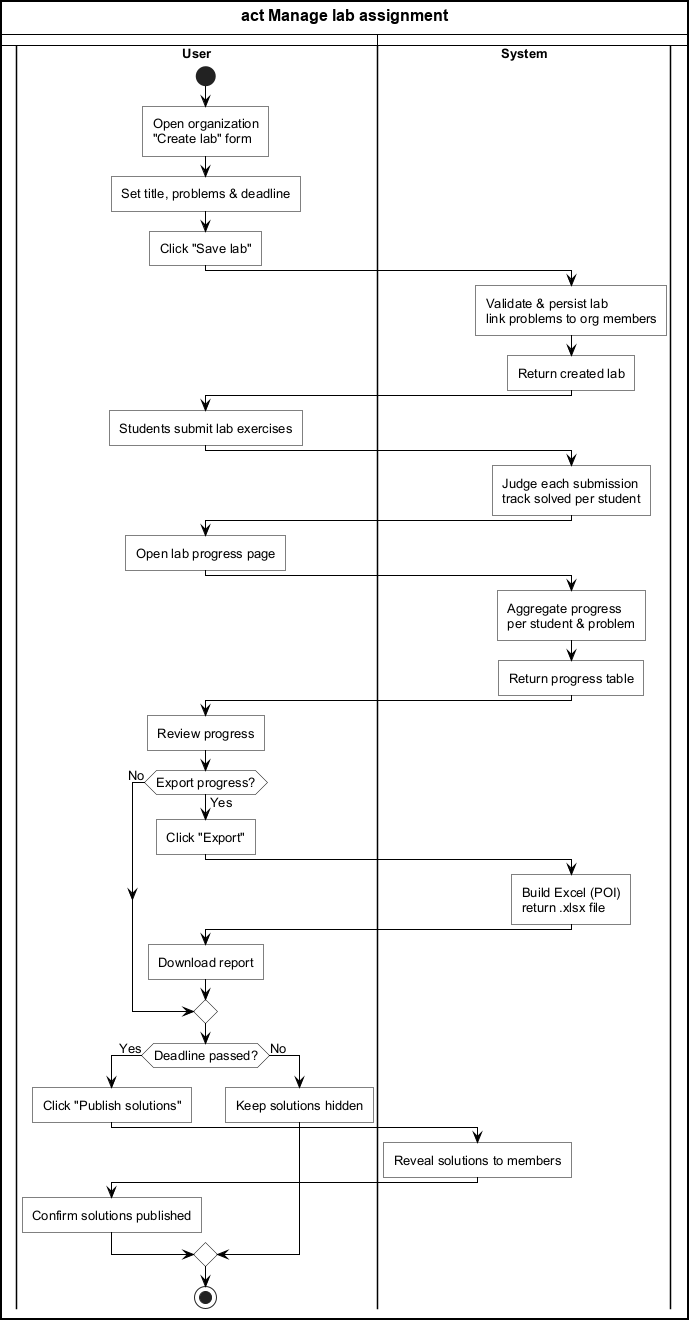
\includegraphics[width=0.70\textwidth,height=0.82\textheight,keepaspectratio]{figures/activity-manage-lab.png}
  \caption{Sơ đồ hoạt động cho Use Case Quản lý bài thực hành}\label{fig:act-uc06}
\end{figure}

Sự tương tác giữa giảng viên và các thành phần của hệ thống được thể hiện qua sơ đồ tuần tự
trong Hình~\ref{fig:seq-uc06}.

\begin{figure}[H]
  \centering
  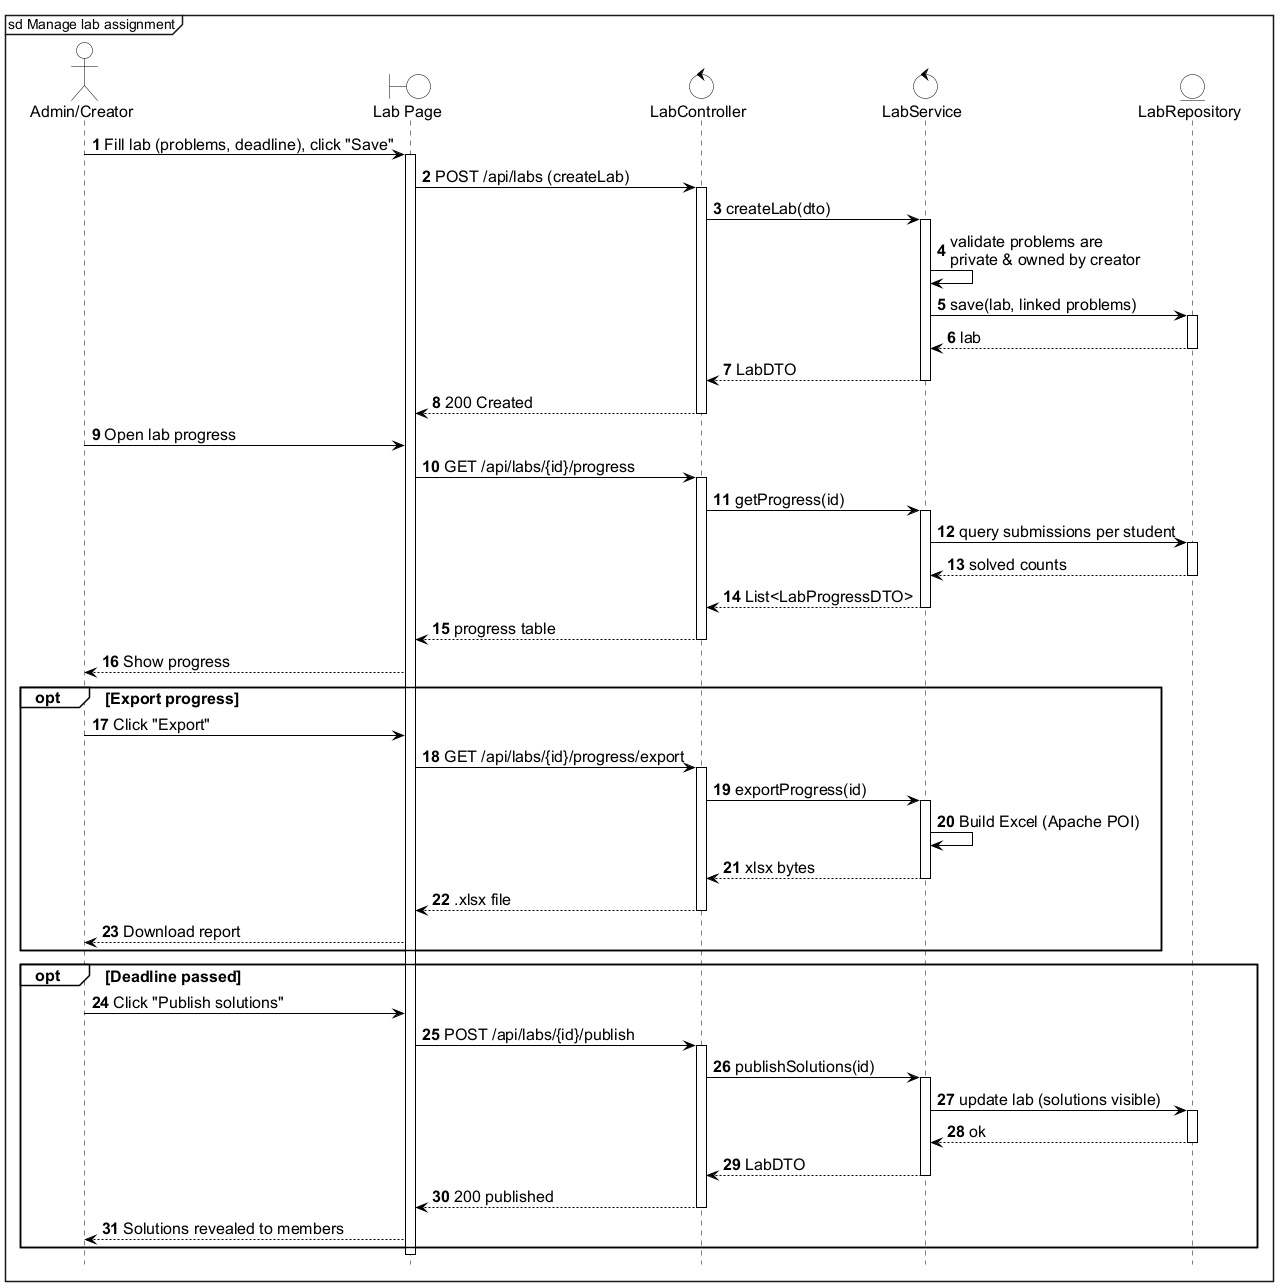
\includegraphics[width=\textwidth]{figures/seq-manage-lab.png}
  \caption{Sơ đồ tuần tự cho Use Case Quản lý bài thực hành}\label{fig:seq-uc06}
\end{figure}

\section{Yêu cầu phi chức năng (Non-functional Requirements)}

Bên cạnh các chức năng nghiệp vụ, hệ thống chấm bài trực tuyến còn phải đáp ứng một số yêu
cầu phi chức năng đặc thù. Do phải tiếp nhận và thực thi mã nguồn không tin cậy từ nhiều người
dùng cùng lúc, đặc biệt trong các kỳ thi, các yêu cầu về hiệu năng, khả năng mở rộng và bảo
mật được đặt lên hàng đầu. Phần này trình bày những yêu cầu phi chức năng chính mà TDTUOJ
hướng tới.

\subsection{Hiệu năng và thời gian phản hồi}

Thao tác nộp bài không được phép làm nghẽn giao diện người dùng. Vì vậy việc chấm bài phải được xử lý
bất đồng bộ: bài nộp được ghi nhận ngay với trạng thái chờ xử lý (PENDING), đưa vào hàng đợi
Redis và do các tiến trình xử lý (worker) lấy ra gửi sang Judge0, nhờ đó người dùng nhận phản
hồi tức thì mà không phải chờ quá trình chấm kết thúc. Các thao tác đọc thường gặp như xem
danh sách bài toán hay bảng xếp hạng được tối ưu bằng bộ nhớ đệm Redis để giảm tải cho cơ sở
dữ liệu. Mỗi bài nộp đều bị ràng buộc giới hạn thời gian và bộ nhớ do Judge0 áp đặt, nhằm đảm bảo
một lời giải sai hoặc kém hiệu quả không thể chiếm dụng tài nguyên vô hạn.

\subsection{Khả năng mở rộng}

Hệ thống được thiết kế để chịu được lượng truy cập và bài nộp tăng đột biến trong thời gian
diễn ra kỳ thi. Phía máy chủ áp dụng cơ chế xác thực phi trạng thái bằng \ac{JWT} nên có thể
nhân bản thành nhiều thực thể và cân bằng tải theo chiều ngang mà không cần chia sẻ phiên làm
việc. Khâu chấm bài được tách rời qua hàng đợi, cho phép tăng số lượng worker và số máy chủ
Judge0 một cách độc lập khi tải tăng. Toàn bộ thành phần được đóng gói bằng Docker, thuận tiện
cho việc triển khai và nhân rộng.

\subsection{Bảo mật}

Bảo mật là yêu cầu trọng yếu do hệ thống thực thi mã nguồn không tin cậy từ người dùng. Mã nguồn nộp
lên luôn được chạy trong môi trường cô lập bằng container của Judge0, tách biệt khỏi máy chủ
ứng dụng nhằm ngăn mã độc truy cập hệ thống hoặc dữ liệu. Việc truy cập được kiểm soát bằng
\ac{JWT} kết hợp phân quyền theo vai trò (User, Contest Creator, Admin) thông qua các chú thích
phân quyền ở mức phương thức của Sping Security; mật khẩu được băm bằng thuật toán BCrypt trước khi lưu. Chính
sách \ac{CORS} giới hạn nguồn gọi \ac{API}, còn tính năng gợi ý bằng \ac{LLM}
được kiểm soát chặt để tránh tiết lộ lời giải hoặc bị lạm dụng ngoài phạm vi học tập.

\subsection{Độ tin cậy và tính sẵn sàng}

Kết quả chấm bài cùng dữ liệu xếp hạng phải chính xác và không được phép mất mát. Trạng thái của
mỗi bài nộp được lưu lại qua các giai đoạn như chờ xử lý, đang chấm và hoàn tất, nên một sự
cố tạm thời của worker hay của Judge0 không làm thất lạc các bài nộp đã được tải lên. Cơ chế chấm bất
đồng bộ qua hàng đợi cũng giúp hệ thống tiếp tục nhận bài ngay cả khi khâu chấm tạm thời quá
tải, các bài nộp dồn lại sẽ được xử lý dần khi tài nguyên trình chấm được giải phóng.

\subsection{Khả năng bảo trì và khả năng sử dụng}

Mã nguồn phía máy chủ được tổ chức theo kiến trúc phân tầng Controller $\to$ Service $\to$ Repository
và chia thành các module theo nghiệp vụ, giúp dễ đọc, dễ kiểm thử và dễ mở rộng tính năng mới.
Toàn bộ \ac{API} được mô tả tự động bằng OpenAPI để thuận tiện cho việc tích hợp và bảo trì.
Về phía người dùng, giao diện hỗ trợ trình soạn thảo mã nguồn Monaco cùng trình minh họa cấu
trúc dữ liệu, mang lại trải nghiệm gần với môi trường lập trình thực tế và hỗ trợ tốt cho mục
tiêu học tập lập trình.

% ============================================================
% CHƯƠNG 4 – THIẾT KẾ HỆ THỐNG
% ============================================================
\chapter{Thiết kế hệ thống}

\section{Thiết kế kiến trúc}

Hệ thống TDTUOJ được xây dựng theo kiến trúc nhiều tầng với sự tách biệt rõ ràng giữa phía
giao diện người dùng (frontend) và phía máy chủ (backend), giao tiếp với nhau qua các giao
diện lập trình ứng dụng (\ac{API}) dạng theo \ac{REST}. Cách tổ chức này giúp hai phía phát triển
và triển khai độc lập, đồng thời thuận tiện cho việc mở rộng theo chiều ngang. Kiến trúc tổng
quan của hệ thống được trình bày trong Hình~\ref{fig:architecture}.

Phía giao diện là một ứng dụng trang đơn (Single Page Application) viết bằng React, tích hợp
trình soạn thảo mã nguồn Monaco; toàn bộ tương tác với máy chủ được thực hiện qua \ac{REST}
trên giao thức \ac{HTTP}. Phía máy chủ là một ứng dụng Spring Boot, gồm tầng bảo mật (xác thực
\ac{JWT} và kiểm soát \ac{CORS}), tầng REST Controller tiếp nhận request, tầng Service xử lý
nghiệp vụ, một tiến trình xử lý bài nộp (worker) chấm bài bất đồng bộ và một WebClient dựa trên
WebFlux để gọi các dịch vụ bên ngoài.

Dữ liệu nghiệp vụ được lưu trong cơ sở dữ liệu quan hệ PostgreSQL, trong khi Redis vừa đóng
vai trò bộ nhớ đệm vừa làm hàng đợi cho khâu chấm bài. Khi tiếp nhận một bài nộp, tầng Service
lưu dữ liệu vào PostgreSQL và đẩy công việc chấm bài vào hàng đợi Redis; tiến trình worker lấy bài nộp
ra khỏi hàng đợi và gửi đến Judge0 (chạy trong Docker) để biên dịch và thực thi. Ngoài ra, hệ
thống còn kết nối tới hai dịch vụ bên ngoài khác là AWS S3 để lưu trữ tập tin đề bài cùng ảnh
đại diện, và Gemini \ac{LLM} để sinh gợi ý và trích xuất đề bài từ tập tin \ac{PDF}.

\begin{figure}[H]
  \centering
  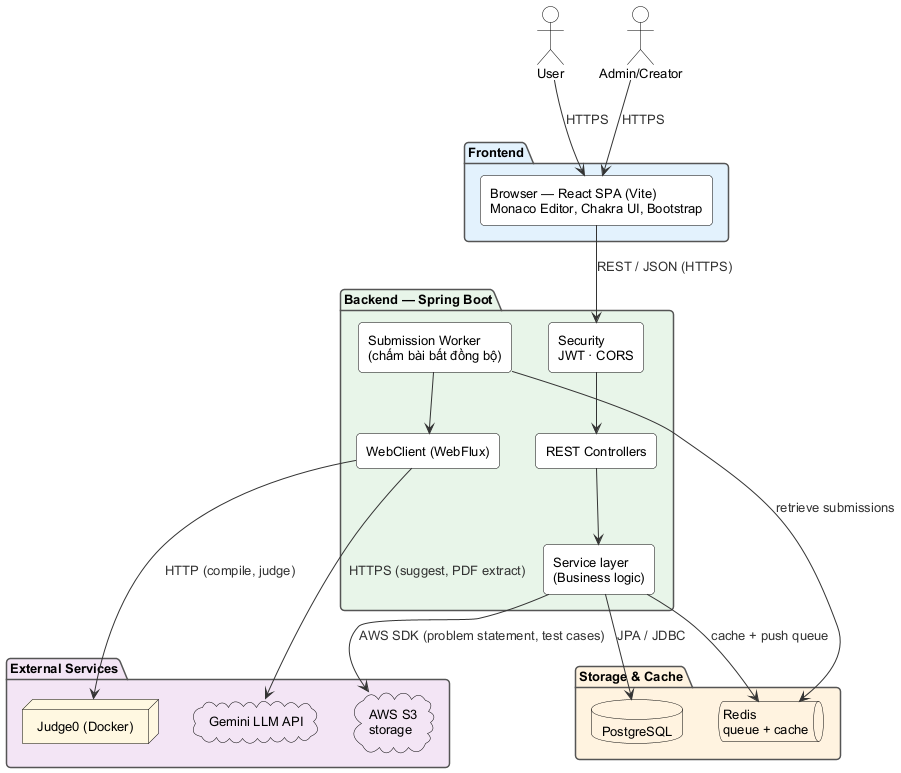
\includegraphics[width=0.95\textwidth,height=0.85\textheight,keepaspectratio]{figures/architecture.png}
  \caption{Kiến trúc tổng quan của hệ thống TDTUOJ}\label{fig:architecture}
\end{figure}

\section{Thiết kế cơ sở dữ liệu / ERD}

\subsection{Tổng quan}

Cơ sở dữ liệu của hệ thống TDTUOJ được xây dựng theo mô hình quan hệ trên hệ quản trị
PostgreSQL, trong đó mỗi thực thể nghiệp vụ được ánh xạ thành một bảng và các quan hệ
được thể hiện thông qua các khóa ngoại. Thiết kế hướng đến bảo đảm tính toàn vẹn dữ liệu trong
các tình huống nhiều bài nộp xử lý đồng thời, đồng thời giữ cấu trúc đơn giản để truy
vấn hiệu quả và mở rộng về sau.

\subsection{Sơ đồ thực thể-quan hệ (ERD)}

Sơ đồ thực thể-quan hệ (\ac{ERD}) là công cụ trực quan mô tả cấu trúc của cơ sở dữ liệu,
gồm ba thành phần chính. Thực thể (entity) tương ứng với một bảng dữ liệu, ví dụ người dùng
hay bài toán. Thuộc tính (attribute) là các cột dữ liệu mô tả một thực thể, chẳng hạn tên đăng
nhập hay địa chỉ thư điện tử. Quan hệ (relationship) thể hiện liên kết giữa các thực thể, cho
biết chúng phối hợp với nhau như thế nào trong nghiệp vụ.

Sơ đồ \ac{ERD} tổng quan của hệ thống được biểu diễn theo ký pháp chân chim (Crow's foot)
trong Hình~\ref{fig:erd}. Trong sơ đồ, mỗi thực thể tương ứng với một bảng, khóa chính được
đánh dấu \ac{PK}, khóa ngoại đánh dấu \ac{FK} và các ràng buộc duy nhất được đánh dấu U; ký pháp
chân chim ở hai đầu đường nối thể hiện lượng số (cardinality) của quan hệ. Toàn bộ lược đồ gồm
hơn hai mươi bảng, được tổ chức xoay quanh một số thực thể trung tâm. Để thuận tiện trình bày,
các mục dưới đây sẽ tách sơ đồ ERD tổng quát thành từng phân mảnh theo thực thể trung tâm và tiến hành mô tả chúng lần lượt;
mỗi mục liệt kê các thuộc tính chính cùng các quan hệ của thực thể tương ứng, trong đó những
bảng liên kết và bảng phụ trợ được trình bày kèm trong phần quan hệ của bảng chủ.

\clearpage
\begin{sidewaysfigure}
  \centering
  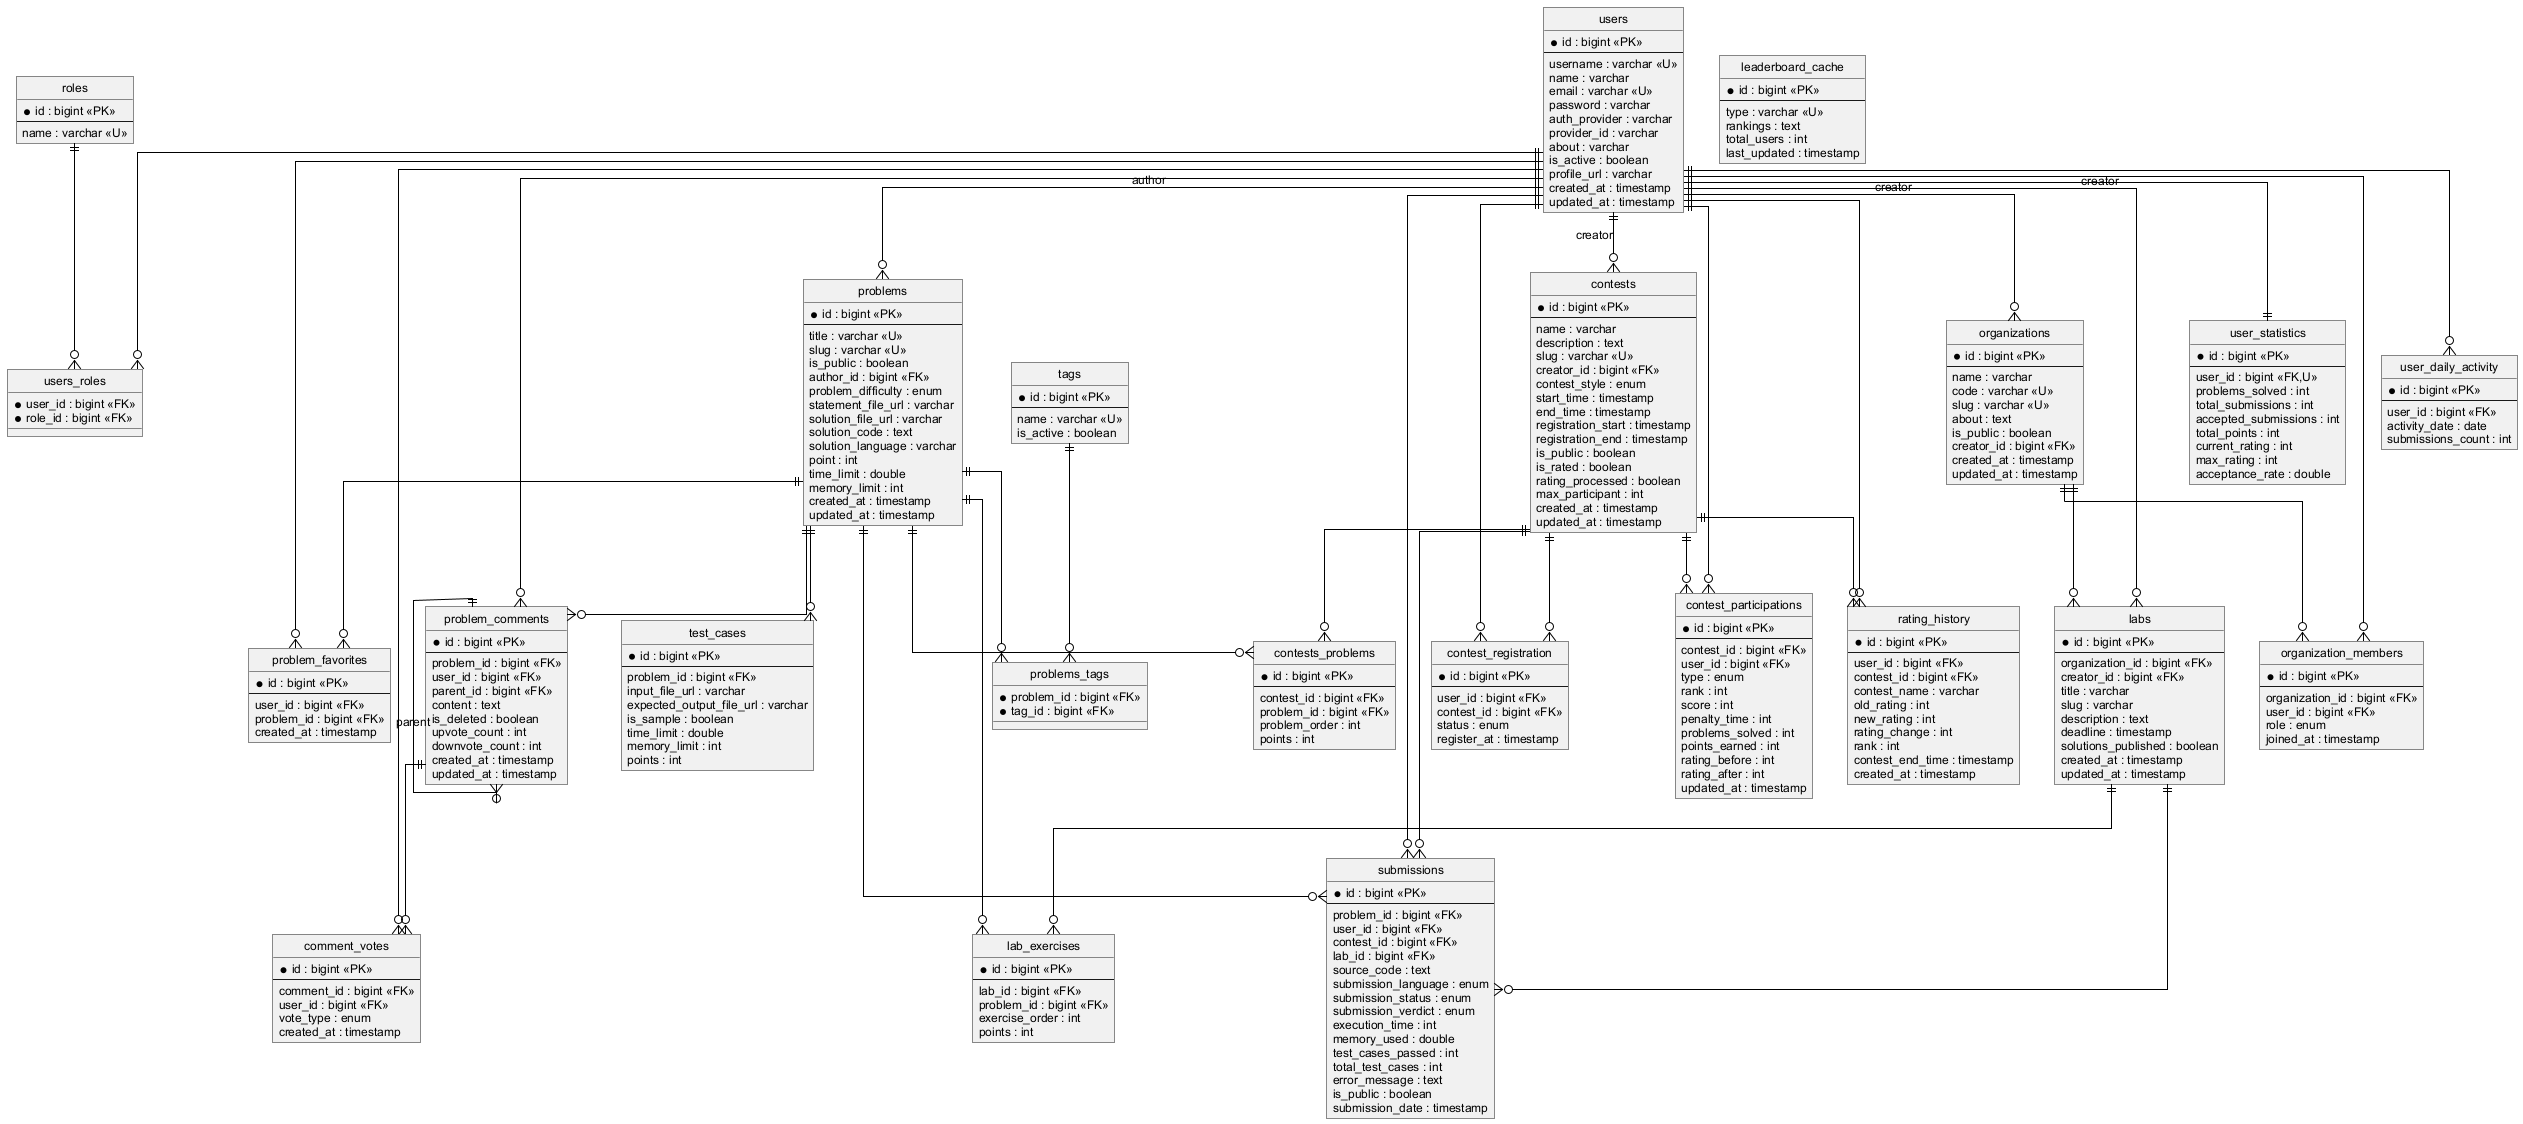
\includegraphics[width=\textheight,height=\textwidth,keepaspectratio]{figures/erd.png}
  \caption{Sơ đồ thực thể-quan hệ tổng quát của hệ thống TDTUOJ}\label{fig:erd}
\end{sidewaysfigure}
\clearpage

\subsubsection{Thực thể Người dùng (User)}

Bảng users là thực thể trung tâm của hệ thống, lưu trữ thông tin tài khoản của mọi
người dùng. Hầu hết hoạt động nghiệp vụ như nộp bài, bình luận, tham gia cuộc thi hay tạo nội
dung đều gắn với một người dùng. Bảng hỗ trợ cả đăng nhập nội bộ và đăng nhập qua nhà cung cấp
bên ngoài thông qua trường auth\_provider. Bảng~\ref{tab:erd-users} mô tả chi tiết
thực thể này. Phân mảnh sơ đồ tương ứng được minh họa trong Hình~\ref{fig:frag-user}.

\begin{figure}[H]
  \centering
  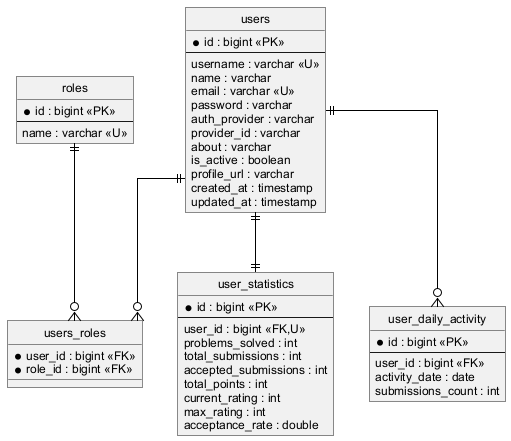
\includegraphics[width=0.95\textwidth,height=0.6\textheight,keepaspectratio]{figures/erd-user.png}
  \caption{Phân mảnh ERD: Người dùng}\label{fig:frag-user}
\end{figure}

\begin{longtable}{|>{\raggedright\arraybackslash}p{3.6cm}|>{\raggedright\arraybackslash}p{8.3cm}|}
  \caption{Mô tả chi tiết thực thể users}\label{tab:erd-users} \\
  \hline
  \endfirsthead
  \hline
  \endhead
  \hline
  \endfoot
  \endlastfoot
  \multicolumn{2}{|l|}{\textbf{Thuộc tính}} \\
  \hline
  id & Khóa chính, định danh người dùng. \\
  \hline
  username & Tên đăng nhập dạng slug, ràng buộc duy nhất. \\
  \hline
  name & Tên hiển thị của người dùng. \\
  \hline
  email & Địa chỉ thư điện tử, ràng buộc duy nhất. \\
  \hline
  password & Mật khẩu đã được băm bằng BCrypt. \\
  \hline
  auth\_provider, provider\_id & Nhà cung cấp đăng nhập (nội bộ hoặc cơ chế OAuth) và định danh tương ứng. \\
  \hline
  about, profile\_url & Giới thiệu ngắn và đường dẫn ảnh đại diện. \\
  \hline
  is\_active & Trạng thái kích hoạt của tài khoản. \\
  \hline
  created\_at, updated\_at & Thời điểm tạo và cập nhật gần nhất. \\
  \hline
  \multicolumn{2}{|l|}{\textbf{Quan hệ}} \\
  \hline
  roles & Nhiều-nhiều với bảng roles thông qua bảng liên kết
    users\_roles; một người dùng có thể mang nhiều vai trò (User, Contest Creator,
    Admin). \\
  \hline
  user\_statistics & Một-một với bảng user\_statistics lưu thống kê tổng
    hợp (số bài đã giải, điểm xếp hạng\dots). \\
  \hline
  user\_daily\_activity & Một-nhiều; ghi nhận số bài nộp theo từng ngày phục vụ
    biểu đồ hoạt động. \\
  \hline
  Nội dung do người dùng tạo & Một-nhiều tới các bảng problems (tác giả),
    submissions, problem\_comments, comment\_votes,
    problem\_favorites và rating\_history. \\
  \hline
\end{longtable}

\subsubsection{Thực thể Bài toán (Problem)}

Bảng problems lưu trữ đề bài cùng các thông số chấm bài. Mỗi bài toán thuộc về một tác
giả, có thể được gắn nhiều thẻ phân loại bài toán, chứa nhiều test case và được sử dụng lại
trong cuộc thi hoặc bài thực hành. Bảng~\ref{tab:erd-problems} mô tả chi tiết thực thể này. Phân mảnh sơ đồ tương ứng được minh họa trong Hình~\ref{fig:frag-problem}.

\begin{figure}[H]
  \centering
  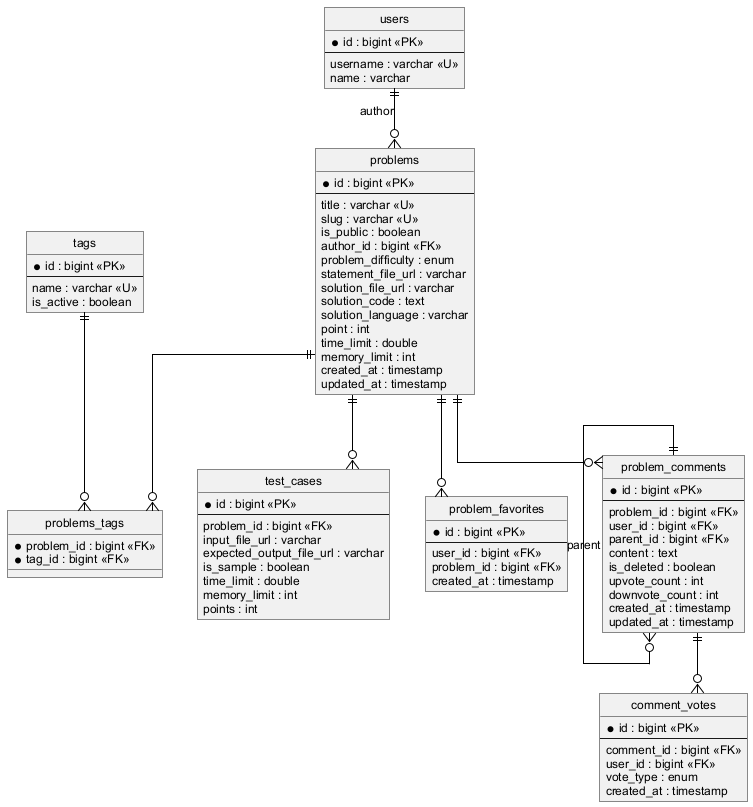
\includegraphics[width=0.95\textwidth,height=0.6\textheight,keepaspectratio]{figures/erd-problem.png}
  \caption{Phân mảnh ERD: Bài toán}\label{fig:frag-problem}
\end{figure}

\begin{longtable}{|>{\raggedright\arraybackslash}p{3.6cm}|>{\raggedright\arraybackslash}p{8.3cm}|}
  \caption{Mô tả chi tiết thực thể problems}\label{tab:erd-problems} \\
  \hline
  \endfirsthead
  \hline
  \endhead
  \hline
  \endfoot
  \endlastfoot
  \multicolumn{2}{|l|}{\textbf{Thuộc tính}} \\
  \hline
  id & Khóa chính, định danh bài toán. \\
  \hline
  title, slug & Tiêu đề và đường dẫn rút gọn, đều có ràng buộc duy nhất. \\
  \hline
  is\_public & Phạm vi hiển thị; bài toán riêng tư chỉ dùng trong cuộc thi hoặc bài
    thực hành. \\
  \hline
  author\_id & Khóa ngoại tới users, là người tạo bài toán. \\
  \hline
  problem\_difficulty & Mức độ khó (EASY, MEDIUM, HARD). \\
  \hline
  statement\_file\_url, solution\_file\_url & Đường dẫn trên S3 tới tập tin
    đề bài và lời giải. \\
  \hline
  solution\_code, solution\_language & Mã nguồn lời giải mẫu và ngôn ngữ
    tương ứng. \\
  \hline
  point & Điểm của bài toán. \\
  \hline
  time\_limit, memory\_limit & Giới hạn thời gian (giây) và bộ nhớ (KB). \\
  \hline
  created\_at, updated\_at & Thời điểm tạo và cập nhật gần nhất. \\
  \hline
  \multicolumn{2}{|l|}{\textbf{Quan hệ}} \\
  \hline
  author & Nhiều-một tới users; mỗi bài toán có một tác giả. \\
  \hline
  test\_cases & Một-nhiều; mỗi bài toán có nhiều trường hợp kiểm thử (đầu vào,
    đầu ra mong đợi, giới hạn, đánh dấu là test case mẫu). \\
  \hline
  tags & Nhiều-nhiều với bảng tags qua bảng liên kết
    problems\_tags. \\
  \hline
  submissions & Một-nhiều; mỗi bài toán nhận nhiều bài nộp. \\
  \hline
  Sử dụng lại & Một-nhiều tới contests\_problems và lab\_exercises khi
    bài toán được đưa vào cuộc thi hoặc bài thực hành. \\
  \hline
  Tương tác người dùng & Một-nhiều tới problem\_comments và
    problem\_favorites. \\
  \hline
\end{longtable}

\subsubsection{Thực thể Bài nộp (Submission)}

Bảng submissions lưu mỗi lần người dùng nộp lời giải cùng kết quả chấm tương ứng. Mỗi
bài nộp luôn gắn với một bài toán và một người dùng; ngoài ra có thể gắn với một cuộc thi hoặc
một bài thực hành tùy theo bối cảnh nộp. Bảng~\ref{tab:erd-submissions} mô tả chi tiết thực thể
này. Phân mảnh sơ đồ tương ứng được minh họa trong Hình~\ref{fig:frag-submission}.

\begin{figure}[H]
  \centering
  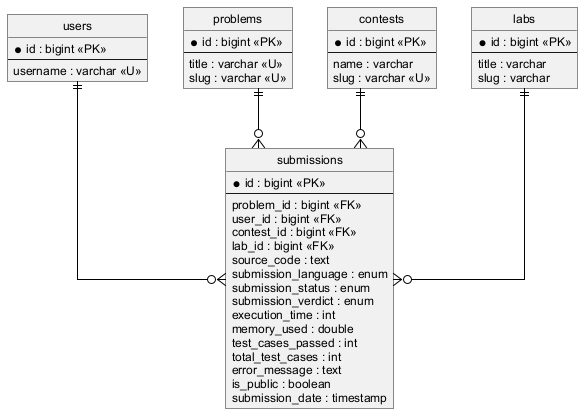
\includegraphics[width=0.95\textwidth,height=0.6\textheight,keepaspectratio]{figures/erd-submission.png}
  \caption{Phân mảnh ERD: Bài nộp}\label{fig:frag-submission}
\end{figure}

\begin{longtable}{|>{\raggedright\arraybackslash}p{3.6cm}|>{\raggedright\arraybackslash}p{8.3cm}|}
  \caption{Mô tả chi tiết thực thể submissions}\label{tab:erd-submissions} \\
  \hline
  \endfirsthead
  \hline
  \endhead
  \hline
  \endfoot
  \endlastfoot
  \multicolumn{2}{|l|}{\textbf{Thuộc tính}} \\
  \hline
  id & Khóa chính, định danh bài nộp. \\
  \hline
  source\_code & Mã nguồn lời giải do người dùng nộp. \\
  \hline
  submission\_language & Ngôn ngữ lập trình (PYTHON, JAVA, JAVASCRIPT, C, CPP, CSHARP). \\
  \hline
  submission\_status & Trạng thái xử lý (PENDING, JUDGING, COMPLETED). \\
  \hline
  submission\_verdict & Kết quả chấm (AC, WA, TLE, MLE, SF, CE, IE). \\
  \hline
  execution\_time, memory\_used & Thời gian thực thi và bộ nhớ sử dụng. \\
  \hline
  test\_cases\_passed, total\_test\_cases & Số trường hợp kiểm thử đã vượt
    qua trên tổng số. \\
  \hline
  error\_message & Thông báo lỗi khi biên dịch hoặc khi chạy (nếu có). \\
  \hline
  is\_public & Cho biết bài nộp có được hiển thị công khai hay không. \\
  \hline
  submission\_date & Thời điểm nộp bài. \\
  \hline
  \multicolumn{2}{|l|}{\textbf{Quan hệ}} \\
  \hline
  problem\_id & Nhiều-một tới problems; bài toán được nộp. \\
  \hline
  user\_id & Nhiều-một tới users; người nộp bài. \\
  \hline
  contest\_id & Nhiều-một tới contests (tùy chọn) khi bài nộp thuộc một
    cuộc thi. \\
  \hline
  lab\_id & Nhiều-một tới labs (tùy chọn) khi bài nộp thuộc một bài thực
    hành. \\
  \hline
\end{longtable}

\subsubsection{Thực thể Cuộc thi (Contest)}

Bảng contests lưu thông tin các cuộc thi tổ chức trên hệ thống, theo thể thức
\ac{ICPC}. Một cuộc thi do một người tạo lập, chứa nhiều bài toán, ghi nhận đăng
ký và quá trình tham gia của người dùng. Bảng~\ref{tab:erd-contests} mô tả chi tiết thực thể
này. Phân mảnh sơ đồ tương ứng được minh họa trong Hình~\ref{fig:frag-contest}.

\begin{figure}[H]
  \centering
  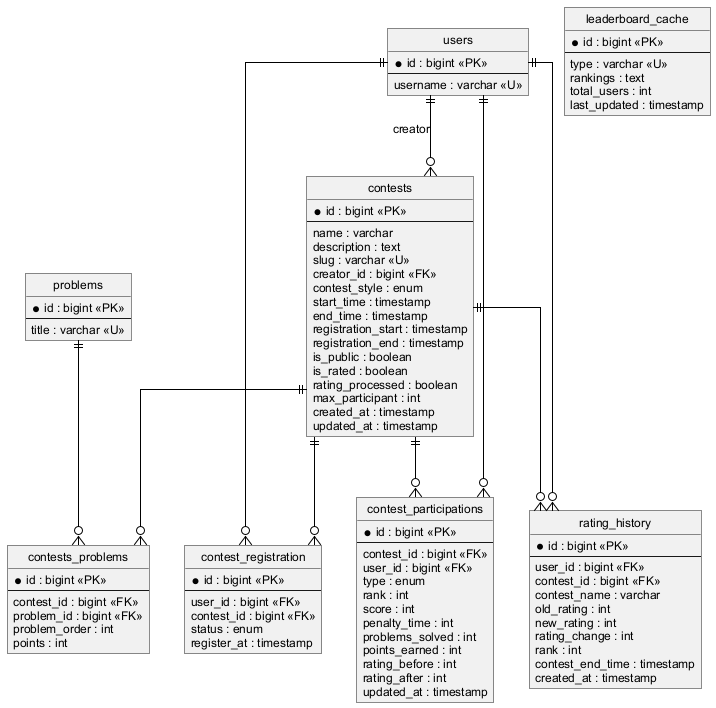
\includegraphics[width=0.95\textwidth,height=0.6\textheight,keepaspectratio]{figures/erd-contest.png}
  \caption{Phân mảnh ERD: Cuộc thi}\label{fig:frag-contest}
\end{figure}

\begin{longtable}{|>{\raggedright\arraybackslash}p{3.6cm}|>{\raggedright\arraybackslash}p{8.3cm}|}
  \caption{Mô tả chi tiết thực thể contests}\label{tab:erd-contests} \\
  \hline
  \endfirsthead
  \hline
  \endhead
  \hline
  \endfoot
  \endlastfoot
  \multicolumn{2}{|l|}{\textbf{Thuộc tính}} \\
  \hline
  id & Khóa chính, định danh cuộc thi. \\
  \hline
  name, slug & Tên cuộc thi và đường dẫn rút gọn (duy nhất). \\
  \hline
  description & Mô tả chi tiết cuộc thi. \\
  \hline
  creator\_id & Khóa ngoại tới users, là người tạo cuộc thi. \\
  \hline
  contest\_style & Thể thức tính điểm (\ac{ICPC}). \\
  \hline
  start\_time, end\_time & Thời gian bắt đầu và kết thúc. \\
  \hline
  registration\_start, registration\_end & Khoảng thời gian mở đăng ký. \\
  \hline
  is\_public, is\_rated & Cuộc thi công khai hay không, có tính điểm xếp
    hạng hay không. \\
  \hline
  rating\_processed & Đánh dấu đã cập nhật điểm xếp hạng sau cuộc thi. \\
  \hline
  freeze\_duration\_minutes & Số phút đóng băng bảng xếp hạng trước khi kết thúc
    (rỗng hoặc 0 nghĩa là không đóng băng). \\
  \hline
  problems\_published & Đánh dấu các bài toán của cuộc thi đã được tự động công khai
    sau khi kết thúc. \\
  \hline
  max\_participant & Số lượng người tham gia tối đa. \\
  \hline
  created\_at, updated\_at & Thời điểm tạo và cập nhật gần nhất. \\
  \hline
  \multicolumn{2}{|l|}{\textbf{Quan hệ}} \\
  \hline
  creator & Nhiều-một tới users; mỗi cuộc thi có một người tạo. \\
  \hline
  contests\_problems & Một-nhiều; liên kết nhiều-nhiều với problems,
    kèm thứ tự và điểm riêng trong cuộc thi. \\
  \hline
  contest\_registration & Một-nhiều; lưu đăng ký tham gia kèm trạng thái phê
    duyệt. \\
  \hline
  contest\_participations & Một-nhiều; lưu điểm, thứ hạng và thời gian phạt (penalty time) của
    từng người tham gia. \\
  \hline
  rating\_history & Một-nhiều; lịch sử thay đổi điểm xếp hạng sau cuộc thi. Bảng
    leaderboard\_cache lưu snapshot bảng xếp hạng dưới dạng JSON, không ràng buộc
    khóa ngoại và khóa cứng. \\
  \hline
\end{longtable}

\subsubsection{Thực thể Tổ chức (Organization)}

Bảng organizations đại diện cho một đơn vị như lớp học hoặc câu lạc bộ, là nơi giảng
viên quản lý thành viên và giao bài thực hành. Bảng~\ref{tab:erd-organizations} mô tả chi tiết
thực thể này. Phân mảnh sơ đồ tương ứng được minh họa trong Hình~\ref{fig:frag-organization}.

\begin{figure}[H]
  \centering
  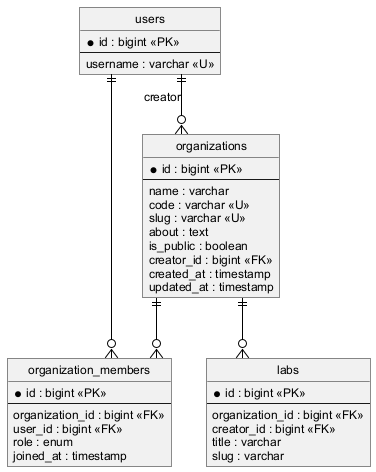
\includegraphics[width=0.95\textwidth,height=0.6\textheight,keepaspectratio]{figures/erd-organization.png}
  \caption{Phân mảnh ERD: Tổ chức}\label{fig:frag-organization}
\end{figure}

\begin{longtable}{|>{\raggedright\arraybackslash}p{3.6cm}|>{\raggedright\arraybackslash}p{8.3cm}|}
  \caption{Mô tả chi tiết thực thể organizations}\label{tab:erd-organizations} \\
  \hline
  \endfirsthead
  \hline
  \endhead
  \hline
  \endfoot
  \endlastfoot
  \multicolumn{2}{|l|}{\textbf{Thuộc tính}} \\
  \hline
  id & Khóa chính, định danh tổ chức. \\
  \hline
  name & Tên tổ chức. \\
  \hline
  code, slug & Mã tham gia và đường dẫn rút gọn, đều ràng buộc duy nhất. \\
  \hline
  about & Giới thiệu về tổ chức. \\
  \hline
  is\_public & Phạm vi hiển thị của tổ chức. \\
  \hline
  creator\_id & Khóa ngoại tới users, là người tạo tổ chức. \\
  \hline
  created\_at, updated\_at & Thời điểm tạo và cập nhật gần nhất. \\
  \hline
  \multicolumn{2}{|l|}{\textbf{Quan hệ}} \\
  \hline
  creator & Nhiều-một tới users; mỗi tổ chức có một người tạo. \\
  \hline
  organization\_members & Một-nhiều; liên kết nhiều-nhiều với users,
    kèm vai trò thành viên (OWNER, ADMIN, MEMBER). \\
  \hline
  labs & Một-nhiều; mỗi tổ chức chứa nhiều bài thực hành. \\
  \hline
\end{longtable}

\subsubsection{Thực thể Bài thực hành (Lab)}

Bảng labs lưu các bài thực hành do giảng viên giao trong phạm vi một tổ chức, gồm
danh sách bài toán và thời hạn nộp. Bảng~\ref{tab:erd-labs} mô tả chi tiết thực thể này. Phân mảnh sơ đồ tương ứng được minh họa trong Hình~\ref{fig:frag-lab}.

\begin{figure}[H]
  \centering
  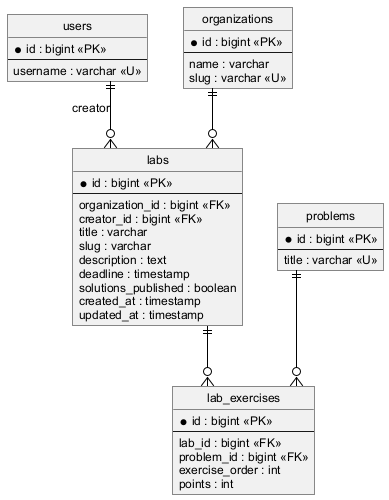
\includegraphics[width=0.95\textwidth,height=0.6\textheight,keepaspectratio]{figures/erd-lab.png}
  \caption{Phân mảnh ERD: Bài thực hành}\label{fig:frag-lab}
\end{figure}

\begin{longtable}{|>{\raggedright\arraybackslash}p{3.6cm}|>{\raggedright\arraybackslash}p{8.3cm}|}
  \caption{Mô tả chi tiết thực thể labs}\label{tab:erd-labs} \\
  \hline
  \endfirsthead
  \hline
  \endhead
  \hline
  \endfoot
  \endlastfoot
  \multicolumn{2}{|l|}{\textbf{Thuộc tính}} \\
  \hline
  id & Khóa chính, định danh bài thực hành. \\
  \hline
  organization\_id & Khóa ngoại tới organizations chứa bài thực hành. \\
  \hline
  creator\_id & Khóa ngoại tới users, là giảng viên tạo bài thực hành. \\
  \hline
  title, slug & Tiêu đề và đường dẫn rút gọn. \\
  \hline
  description & Mô tả nội dung bài thực hành. \\
  \hline
  deadline & Thời hạn nộp bài. \\
  \hline
  solutions\_published & Đánh dấu lời giải đã được công bố cho thành viên hay
    chưa. \\
  \hline
  created\_at, updated\_at & Thời điểm tạo và cập nhật gần nhất. \\
  \hline
  \multicolumn{2}{|l|}{\textbf{Quan hệ}} \\
  \hline
  organization & Nhiều-một tới organizations. \\
  \hline
  creator & Nhiều-một tới users. \\
  \hline
  lab\_exercises & Một-nhiều; liên kết nhiều-nhiều với problems, kèm
    thứ tự và điểm của từng bài trong bài thực hành. \\
  \hline
\end{longtable}

\section{Thiết kế giao diện}

Giao diện người dùng được xây dựng bằng React theo mô hình thành phần (component),
kết hợp hai thư viện trình bày là Chakra UI và Bootstrap. Toàn bộ ứng dụng tuân theo
một thiết kế thống nhất với nền tối, màu nhấn vàng cam và thanh điều hướng cố
định ở đầu trang, nhờ đó người dùng dễ dàng di chuyển giữa các phần như bài toán, cuộc
thi, tổ chức và người dùng. Bố cục được thiết kế theo hướng đáp ứng (responsive), tự
điều chỉnh theo kích thước màn hình, đồng thời ưu tiên tính rõ ràng của thông tin nhằm
phục vụ thao tác luyện tập và thi đấu. Các tiểu mục dưới đây trình bày những màn hình
tiêu biểu của hệ thống.

\subsection{Trang chi tiết bài toán và nộp bài}

Trang chi tiết bài toán là màn hình làm việc trọng tâm của người dùng, được chia thành hai
khu vực như Hình~\ref{fig:ui-problem-detail}. Khu vực bên trái trình bày đề bài gồm phát
biểu, định dạng dữ liệu vào/ra và các bộ dữ liệu mẫu. Khu vực bên phải là trình soạn
thảo mã nguồn Monaco, cho phép chọn ngôn ngữ lập trình và viết lời giải trực tiếp trên
trình duyệt. Khi người dùng nộp bài, mã nguồn được gửi tới hệ thống chấm và kết quả được
hiển thị ở bảng phía dưới: trong hình ví dụ này, lời giải được chấm đạt toàn bộ hai trên hai test case kèm thông tin thời gian và bộ nhớ tiêu thụ.

\begin{figure}[H]
  \centering
  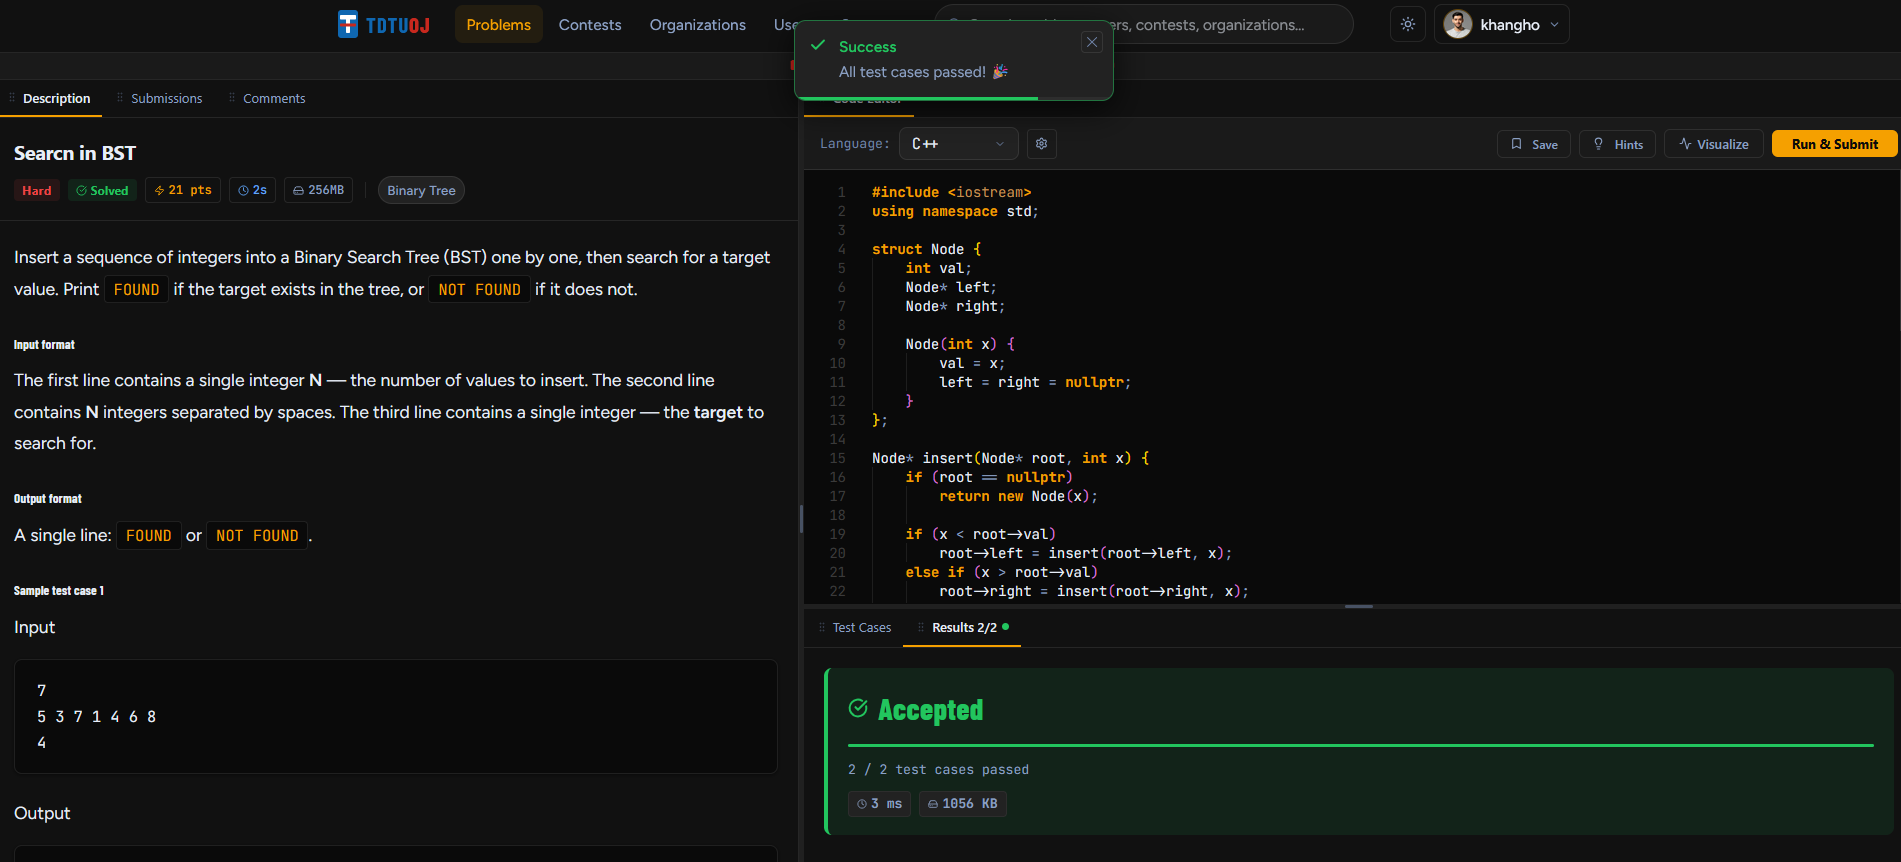
\includegraphics[width=\textwidth]{figures/ui-problem-detail.png}
  \caption{Giao diện trang chi tiết bài toán và kết quả nộp bài}\label{fig:ui-problem-detail}
\end{figure}

\subsection{Trang cuộc thi và bảng xếp hạng}

Trang cuộc thi cung cấp thông tin chi tiết của một cuộc thi cùng bảng xếp hạng theo thời
gian thực. Như Hình~\ref{fig:ui-contest} thể hiện, đầu trang hiển thị tên, thể thức, thời
gian diễn ra và trạng thái của cuộc thi, kèm bảng thông tin tóm tắt ở cạnh phải. Phần thân
trang gồm hai thẻ là danh sách bài toán và bảng xếp hạng; bảng xếp hạng liệt kê thứ hạng,
tên thí sinh, số bài giải được và điểm phạt, được cập nhật tự động trong suốt quá trình thi
đấu.

\begin{figure}[H]
  \centering
  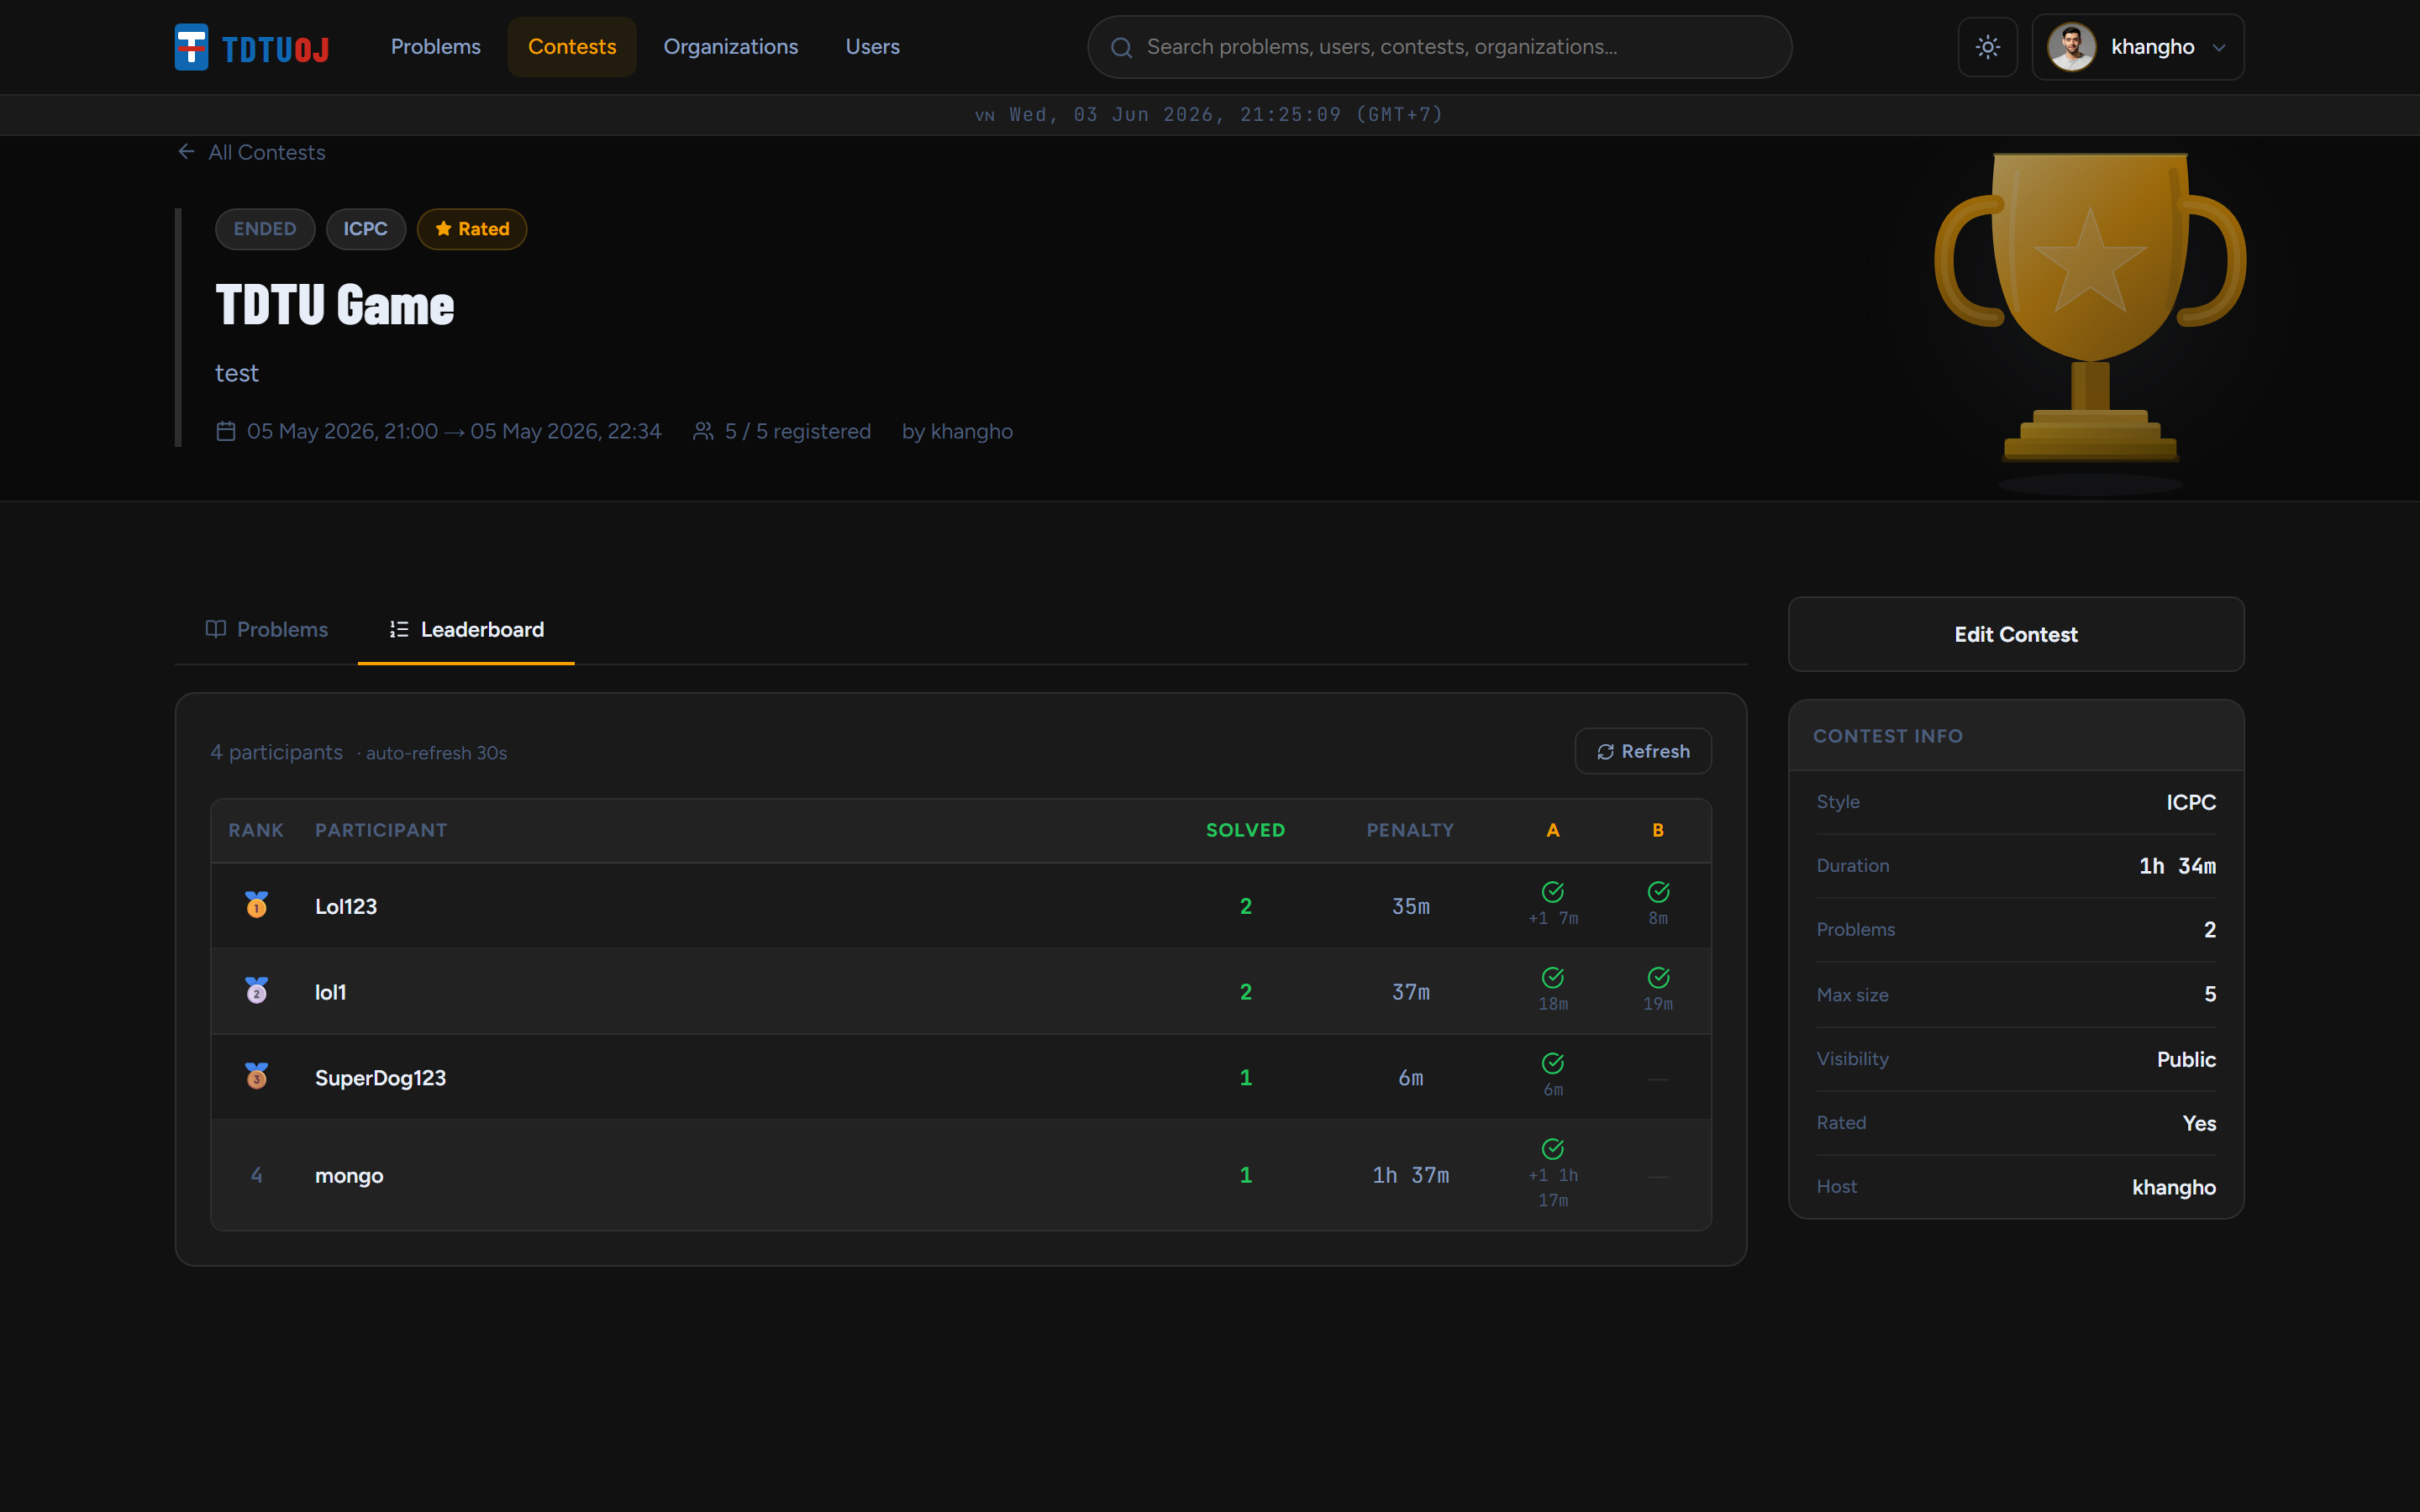
\includegraphics[width=\textwidth]{figures/ui-contest.png}
  \caption{Giao diện trang cuộc thi và bảng xếp hạng}\label{fig:ui-contest}
\end{figure}

\subsection{Trang quản trị}

Trang quản trị dành cho quản trị viên và giảng viên, tập hợp các chức năng quản lý nội dung
của hệ thống. Như Hình~\ref{fig:ui-admin} minh họa, giao diện hiển thị phần dashboard của trang quản trị
cho phép admin xem các chỉ số liên quan đến hệ thống như số người dùng, số bài toán, và các phân tích về lần nộp bài
của người dùng qua thời gian.

\begin{figure}[H]
  \centering
  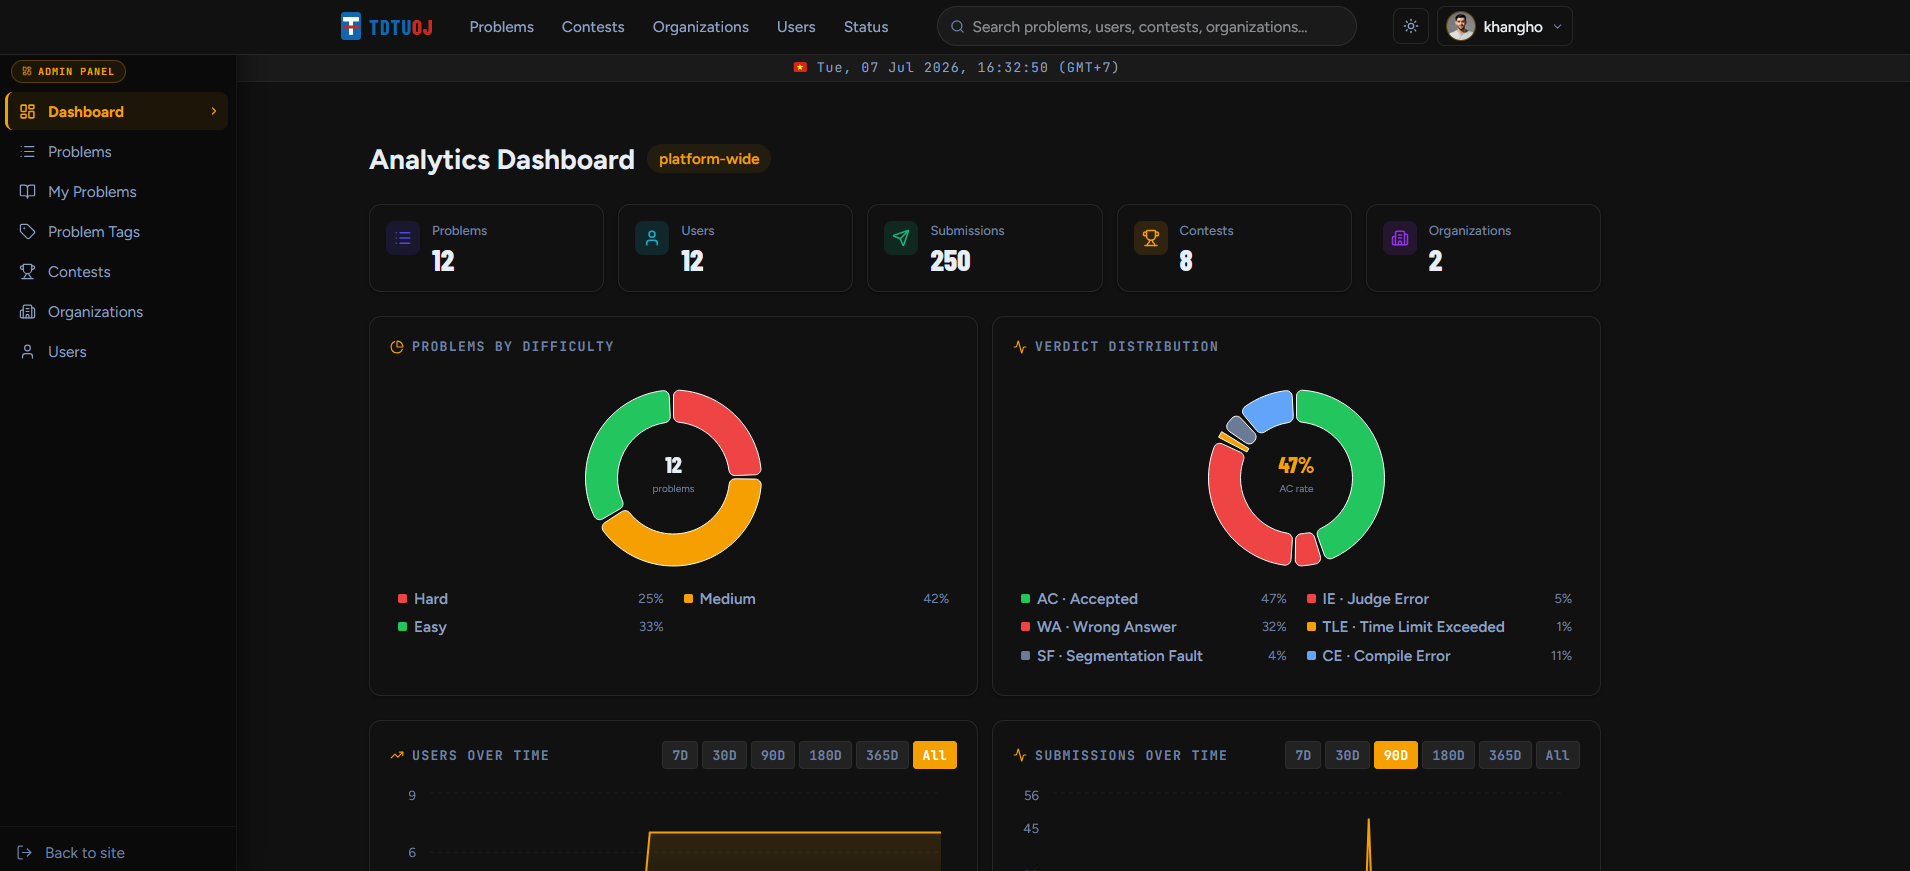
\includegraphics[width=\textwidth]{figures/ui-admin.png}
  \caption{Giao diện trang quản trị bài toán}\label{fig:ui-admin}
\end{figure}

\subsection{Trang trực quan hóa cấu trúc dữ liệu}

Trình minh họa cấu trúc dữ liệu là một cửa sổ phụ mở ra ngay trên màn hình làm bài. Như
Hình~\ref{fig:ui-visualizer} mô tả, cửa sổ chia thành hai phần: bên trái là mã nguồn của
người dùng với dòng đang thực thi được tô sáng, bên phải là khung minh họa cấu trúc dữ liệu
được phát hiện tự động từ dữ liệu trong quá trình chạy. Trong hình đang hiển thị cấu trúc cây nhị phân tìm kiếm từ mã nguồn mà người dùng nộp cho bài toán. 
Thanh điều khiển phía dưới cho phép phát lại từng bước thực thi như một đoạn hoạt ảnh, 
đồng thời khu vực kết quả hiển thị dữ liệu xuất ra của chương trình, hỗ trợ người học quan sát trực quan các bước của thuật toán.

\begin{figure}[H]
  \centering
  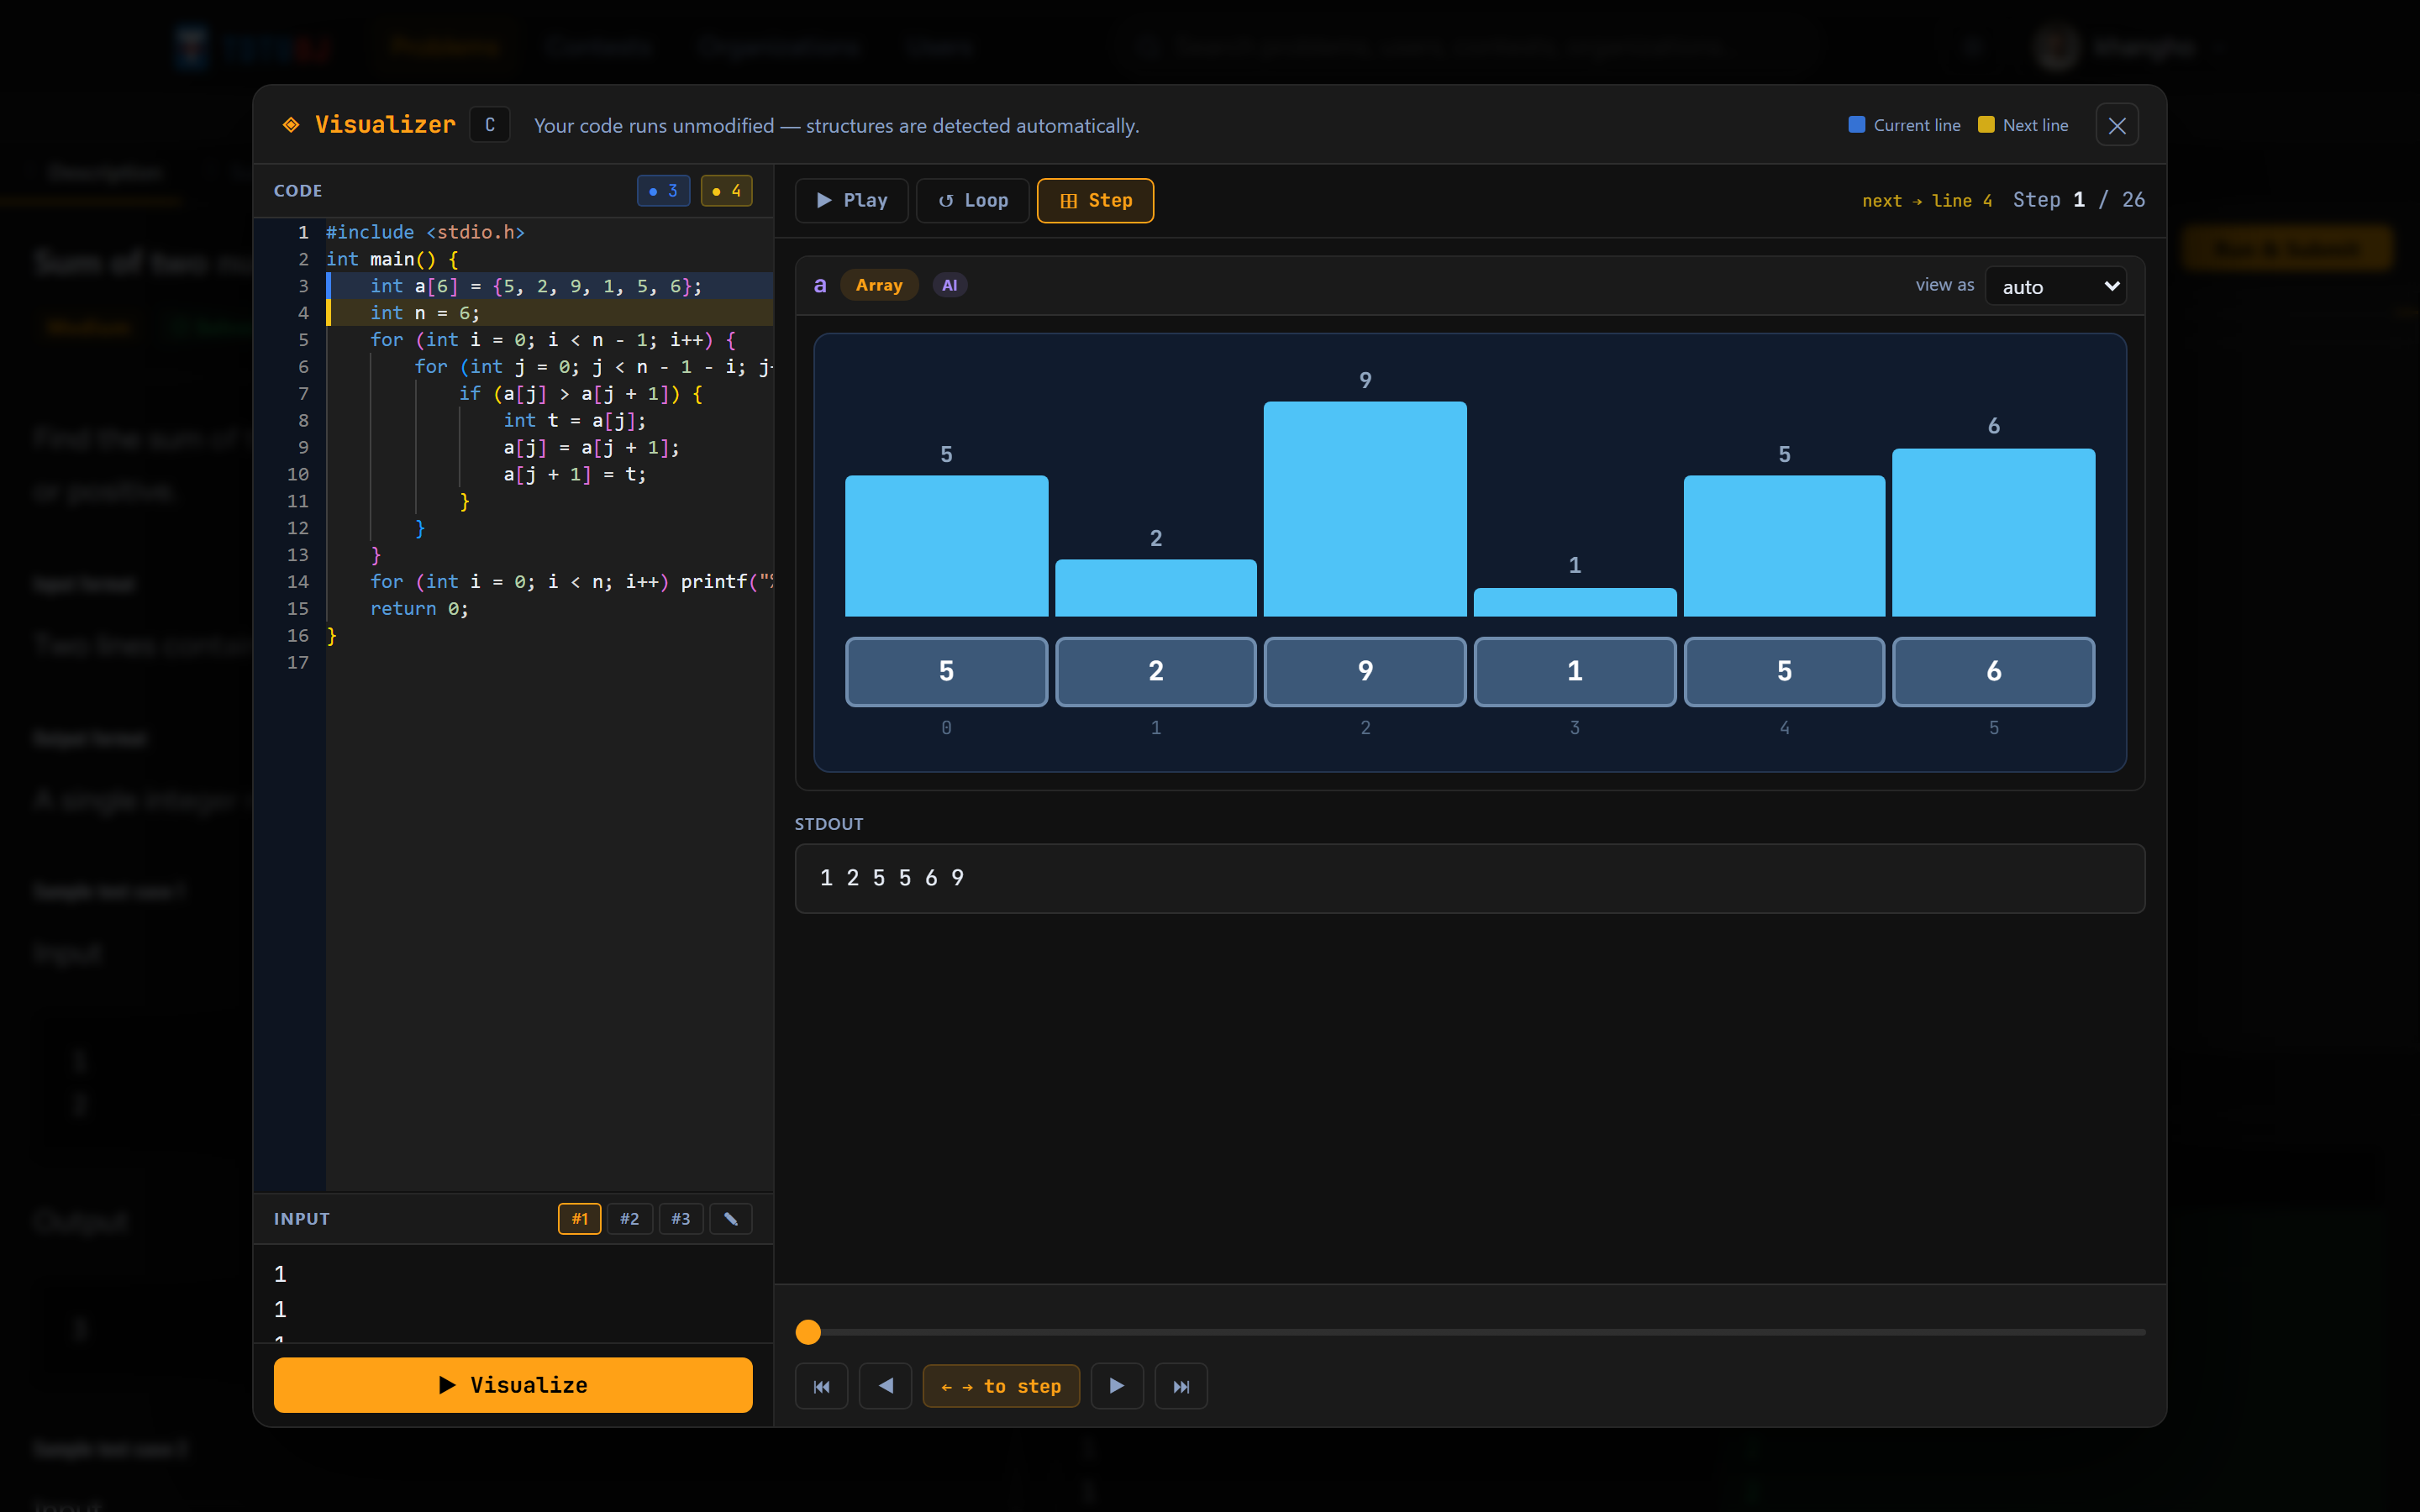
\includegraphics[width=\textwidth]{figures/ui-visualizer.png}
  \caption{Giao diện trình minh họa cấu trúc dữ liệu}\label{fig:ui-visualizer}
\end{figure}

\subsection{Trang theo dõi tiến độ bài thực hành}

Trang theo dõi tiến độ hỗ trợ giảng viên giám sát kết quả làm bài của sinh viên trong một bài
thực hành. Như Hình~\ref{fig:ui-lab-progress} thể hiện, đầu trang tổng hợp các chỉ số chung
như số sinh viên, số bài toán, tỷ lệ hoàn thành trung bình và sinh viên đạt điểm cao nhất.
Bảng bên dưới hiển thị tiến độ chi tiết của từng sinh viên theo từng bài toán, đánh dấu trạng
thái đã giải kèm điểm số đạt được. Giao diện còn cho phép xuất dữ liệu tiến độ ra tệp định
dạng \ac{CSV} hoặc Excel để phục vụ việc đánh giá và lưu trữ.

\begin{figure}[H]
  \centering
  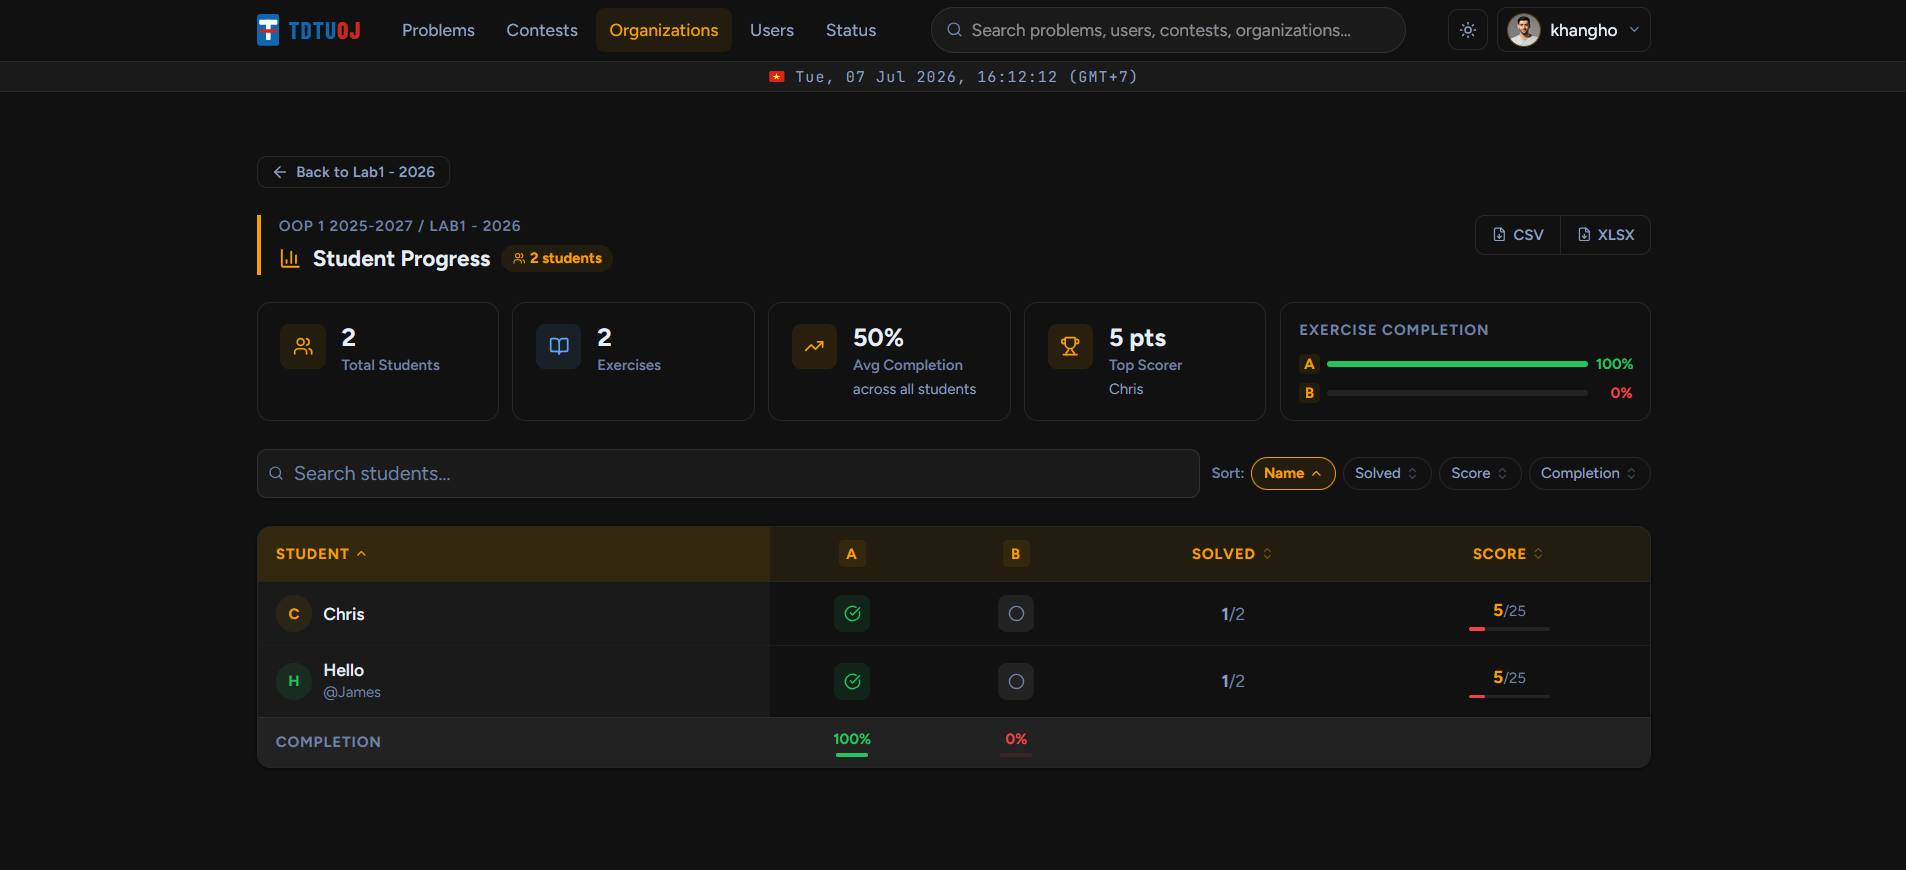
\includegraphics[width=\textwidth]{figures/ui-lab-progress.png}
  \caption{Giao diện trang theo dõi tiến độ bài thực hành}\label{fig:ui-lab-progress}
\end{figure}

\section{Thiết kế hiệu năng và bảo mật}

Bên cạnh các thiết kế về kiến trúc, dữ liệu và giao diện, hệ thống TDTUOJ còn được thiết kế
nhằm đáp ứng hai yêu cầu phi chức năng trọng yếu đã nêu ở Chương~3 là bảo mật và hiệu năng
khi phục vụ nhiều người dùng đồng thời. Mục này trình bày hai cơ chế cốt lõi tương ứng: xác
thực phi trạng thái bằng \ac{JWT} và giới hạn tần suất truy cập (rate limiting) dựa trên Redis.
Cả hai cơ chế được hiện thực dưới dạng bộ lọc (filter) đặt trước tầng điều khiển, nhờ đó áp
dụng nhất quán cho toàn bộ các request \ac{REST} mà không xen lẫn vào mã nghiệp vụ.

\subsection{Xác thực và phân quyền bằng JWT}

Hệ thống xác thực người dùng theo cơ chế phi trạng thái (stateless), nghĩa là máy chủ không
lưu phiên đăng nhập. Sau khi người dùng đăng nhập thành công, máy chủ cấp cho họ một mã thông
báo \ac{JWT}. Mã này do lớp \textit{JwtUtils} sinh ra bằng thuật toán HMAC-SHA256 và chứa ba
thông tin chính: định danh người dùng (địa chỉ thư điện tử), thời điểm phát hành và thời hạn
hiệu lực. Phía giao diện lưu lại mã thông báo, rồi gửi kèm nó trong tiêu đề
\textit{Authorization} theo dạng \textit{Bearer} ở mỗi request kế tiếp.

Hình~\ref{fig:jwt-flow} mô tả toàn bộ luồng xác thực bằng sơ đồ tuần tự, từ lúc người dùng
đăng nhập cho đến khi một request mang mã thông báo được kiểm tra và cho phép truy cập.

\begin{figure}[H]
  \centering
  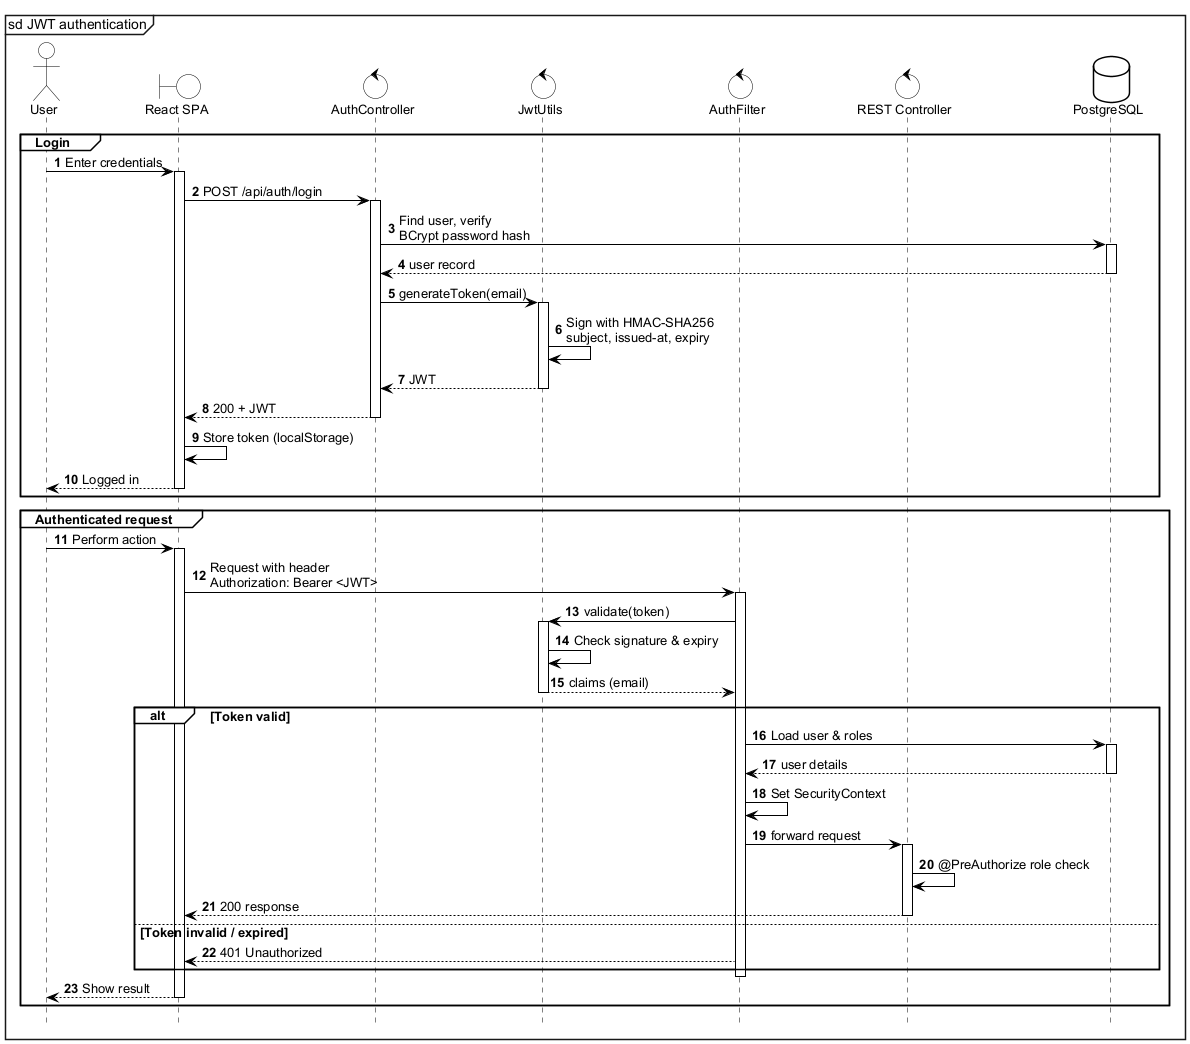
\includegraphics[width=\textwidth]{figures/jwt-flow.png}
  \caption{Sơ đồ tuần tự luồng xác thực và phân quyền bằng \ac{JWT}}\label{fig:jwt-flow}
\end{figure}

Mỗi request gửi đến đều đi qua bộ lọc \textit{AuthFilter}. Bộ lọc này lấy mã thông báo từ
tiêu đề \textit{Authorization}, kiểm tra chữ ký và thời hạn, sau đó nạp thông tin người dùng
từ cơ sở dữ liệu và thiết lập ngữ cảnh bảo mật cho Spring Security. Nếu mã thông báo sai hoặc
đã hết hạn, máy chủ từ chối request và trả về mã trạng thái \ac{HTTP} 401. Việc phân quyền
dựa trên ba vai trò ADMIN, CREATOR và PARTICIPANT, được kiểm soát ở từng phương thức bằng chú
thích \textit{@PreAuthorize}. Vì máy chủ không lưu phiên đăng nhập, hệ thống có thể dễ dàng mở
rộng bằng cách chạy thêm nhiều máy chủ song song.

\subsection{Giới hạn tần suất truy cập với Redis}

Để tránh bị lạm dụng và để bảo vệ những tác vụ tốn nhiều tài nguyên như trình chấm hay API
\ac{LLM}, hệ thống giới hạn số request mà mỗi người dùng được gửi trong một khoảng thời gian nhất định.
Cơ chế này dựa trên thuật toán token bucket của thư viện Bucket4j. Trạng thái
của mỗi bucket được lưu tập trung trên Redis, nhờ đó hạn mức vẫn được áp dụng đồng nhất khi hệ
thống chạy trên nhiều máy chủ.

Cơ chế được cài đặt bằng bộ lọc \textit{RateLimitFilter}, đặt ngay sau \textit{AuthFilter} để
biết ai là người gửi request. Mỗi người dùng được nhận diện bằng một khóa riêng: người đã
đăng nhập dùng khóa theo mã tài khoản, còn người ẩn danh dùng khóa theo địa chỉ IP. Tùy theo
loại thao tác, ví dụ đăng nhập, nộp bài hay gọi \ac{LLM}, mỗi request được xếp vào một bậc
giới hạn (tier). Mỗi bậc quy định số request tối đa cho phép trong một cửa sổ thời gian, tách
riêng cho người ẩn danh và người đã đăng nhập. Bảng~\ref{tab:ratelimit-tiers} liệt kê cấu hình
của các bậc này. Trong bảng, giá trị 0 nghĩa là loại người dùng đó bị chặn hoàn toàn khỏi nhóm
chức năng tương ứng, ví dụ người dùng ẩn danh không được dùng tính năng \ac{LLM}.

\begin{table}[H]
  \centering
  \begin{tabular}{|l|>{\raggedright\arraybackslash}p{5.2cm}|c|c|c|}
    \hline
    \multirow{2}{*}{\textbf{Bậc}} & \multirow{2}{*}{\textbf{Phạm vi áp dụng}}
      & \multicolumn{2}{c|}{\textbf{Số request tối đa mỗi cửa sổ}}
      & \multirow{2}{*}{\textbf{Cửa sổ (giây)}} \\
    \cline{3-4}
    & & \textbf{Ẩn danh} & \textbf{Đã xác thực} & \\
    \hline
    default & Các request còn lại & 60 & 120 & 60 \\
    \hline
    read-heavy & GET danh sách bài toán, cuộc thi, người dùng, tổ chức & 120 & 240 & 60 \\
    \hline
    auth & Đăng nhập, đăng ký, đăng nhập Google & 5 & 10 & 60 \\
    \hline
    submission & Nộp bài (\textit{POST /api/submissions/**}) & 3 & 10 & 60 \\
    \hline
    visualizer & Trực quan hóa (\textit{POST /api/visualize}) & 5 & 20 & 60 \\
    \hline
    AI & Gợi ý và trích xuất bằng \ac{LLM} & 0 & 10 & 60 \\
    \hline
    admin & Các request quản trị (\textit{/api/admin/**}) & 0 & 300 & 60 \\
    \hline
  \end{tabular}
  \caption{Cấu hình các bậc giới hạn tần suất truy cập}\label{tab:ratelimit-tiers}
\end{table}

Khi một request được chấp nhận, máy chủ gắn thêm các tiêu đề \textit{X-RateLimit-Limit} và
\textit{X-RateLimit-Remaining} để phía giao diện biết hạn mức còn lại. Khi vượt hạn mức, máy
chủ trả về mã trạng thái \ac{HTTP} 429 kèm tiêu đề \textit{Retry-After} cho biết thời gian cần
chờ trước khi gửi lại. Bộ lọc được thiết kế theo nguyên tắc ưu tiên tính sẵn sàng
(\emph{fail-open}): nếu Redis gặp sự cố, request vẫn được cho đi qua thay vì bị chặn. Ngoài ra,
hệ thống còn thu thập số liệu về số request được chấp nhận, bị từ chối và số lỗi Redis (qua
\textit{RateLimitMetrics}) để phục vụ giám sát.

% ============================================================
% CHƯƠNG 5 – CÀI ĐẶT VÀ KIỂM THỬ
% ============================================================
\chapter{Cài đặt và kiểm thử}

Chương này trình bày quá trình cài đặt hệ thống TDTUOJ và công tác kiểm thử nhằm bảo đảm
chất lượng. Phần đầu mô tả môi trường, công cụ và cách tổ chức mã nguồn theo tầng, tập
trung vào luồng nghiệp vụ tiêu biểu là nộp bài và chấm bài. Phần sau trình bày hai phần
kiểm thử: kiểm thử đơn vị cho tầng nghiệp vụ và kiểm thử tải kết hợp giám sát hệ thống.

\section{Môi trường và công cụ cài đặt}

Hệ thống được phát triển và chạy thử trên một máy tính cá nhân. Phía máy chủ (backend) và phía
giao diện (frontend) chạy độc lập, giao tiếp với nhau qua các giao diện lập trình ứng dụng
(\ac{API}) dạng \ac{REST}. Phía máy chủ là một ứng dụng Spring Boot viết bằng Java 21, được
biên dịch và chạy bằng Maven. Phía giao diện là một ứng dụng React, được dựng
và chạy bằng Vite qua trình quản lý gói npm. Ngoài ra, các dịch vụ phụ trợ được đóng gói và
chạy trong Docker để dễ cài đặt và thiết lập. Bảng~\ref{tab:env} liệt kê các thành phần chính
cùng công cụ và cổng dịch vụ tương ứng.

\begin{table}[H]
  \centering
  \begin{tabular}{|>{\raggedright\arraybackslash}p{4.2cm}|>{\raggedright\arraybackslash}p{6.5cm}|>{\raggedright\arraybackslash}p{2.3cm}|}
    \hline
    \multicolumn{1}{|c|}{\textbf{Thành phần}}
      & \multicolumn{1}{c|}{\textbf{Công nghệ}}
      & \multicolumn{1}{c|}{\textbf{Cổng}} \\
    \hline
    Phía máy chủ        & Spring Boot (Java 21), Maven    & 8090 \\
    \hline
    Phía giao diện      & React, Vite                     & 5173 \\
    \hline
    Cơ sở dữ liệu       & PostgreSQL                      & 5431 \\
    \hline
    Bộ nhớ đệm, hàng đợi & Redis                          & 6379 \\
    \hline
    Dịch vụ chấm bài    & Judge0 (Docker)                 & 2358 \\
    \hline
  \end{tabular}
  \caption{Các thành phần trong môi trường cài đặt}\label{tab:env}
\end{table}

\section{Cài đặt hệ thống}

\subsection{Tổ chức mã nguồn theo tầng}

Mã nguồn phía máy chủ được tổ chức theo mô hình phân tầng quen thuộc của Spring Boot. Mỗi phân
hệ nghiệp vụ là một gói (package) riêng và chứa đầy đủ các tầng. Tầng điều khiển (Controller)
tiếp nhận request \ac{REST} rồi trả về phản hồi. Tầng dịch vụ (Service) chứa logic nghiệp vụ,
được tách thành phần giao diện và lớp cài đặt *Impl. Tầng kho dữ liệu (Repository) truy xuất cơ
sở dữ liệu qua Spring Data \ac{JPA}. Dữ liệu được biểu diễn bằng hai loại đối tượng: thực thể
(Entity) ánh xạ trực tiếp với bảng trong cơ sở dữ liệu, còn đối tượng truyền dữ liệu (Data
Transfer Object, DTO) dùng để trao đổi với phía giao diện; thư viện ModelMapper đảm nhận việc
chuyển đổi giữa hai loại. Cách phân chia này tương ứng với khuôn mẫu \ac{MVC}, nhờ đó trách
nhiệm của từng tầng được phân chia rõ ràng. Bảng~\ref{tab:layers} tóm tắt vai trò của từng tầng,
lấy ví dụ là một lớp tiêu biểu.

\begin{table}[H]
  \centering
  \begin{tabular}{|>{\raggedright\arraybackslash}p{2.6cm}|>{\raggedright\arraybackslash}p{6.2cm}|>{\footnotesize\raggedright\arraybackslash}p{3.6cm}|}
    \hline
    \multicolumn{1}{|c|}{\textbf{Tầng}}
      & \multicolumn{1}{c|}{\textbf{Trách nhiệm}}
      & \multicolumn{1}{c|}{\textbf{Lớp ví dụ}} \\
    \hline
    Controller & Tiếp nhận request \ac{REST}, kiểm tra đầu vào, trả phản hồi
      & SubmissionController \\
    \hline
    Service & Xử lý logic nghiệp vụ (giao diện và lớp cài đặt)
      & SubmissionServiceImpl \\
    \hline
    Repository & Truy xuất cơ sở dữ liệu qua Spring Data \ac{JPA}
      & SubmissionRepository \\
    \hline
    Entity & Ánh xạ đối tượng với bảng dữ liệu
      & Submission \\
    \hline
    DTO & Truyền dữ liệu giữa các tầng và với phía giao diện
      & SubmissionDTO \\
    \hline
  \end{tabular}
  \caption{Các tầng trong mã nguồn phía máy chủ}\label{tab:layers}
\end{table}

Để bảo đảm tính nhất quán, mọi phản hồi từ phía máy chủ đều được bọc trong một lớp vỏ chung
Response<T> gồm mã trạng thái, thông điệp và dữ liệu. Các lỗi phát sinh được xử lý tập trung
tại lớp GlobalExceptionHandler. Việc xác thực và phân quyền do bộ lọc AuthFilter kết hợp
\ac{JWT} đảm nhận, kiểm tra mã thông báo trước khi request đến tầng điều khiển. Các phân hệ
quản lý dữ liệu khác như bài toán, cuộc thi, tổ chức và bài thực hành đều theo cùng khuôn mẫu
này nên nhóm không trình bày lại.

\subsection{Luồng nộp bài và chấm bài bất đồng bộ}\label{subsec:submit-flow}

Nộp bài và chấm bài là luồng nghiệp vụ quan trọng nhất, đồng thời minh họa rõ cách các tầng
phối hợp với nhau. Khi người dùng nộp một lời giải, SubmissionController chuyển request cho
SubmissionServiceImpl. Lớp này kiểm tra các điều kiện như khoảng chờ giữa hai lần nộp và quyền
tham gia cuộc thi, sau đó lưu bản ghi bài nộp ở trạng thái chờ và đẩy một công việc vào hàng
đợi trên Redis thông qua SubmissionQueueService. Việc chấm bài không diễn ra ngay trong luồng
xử lý request mà được thực hiện bất đồng bộ. Cụ thể, một tiến trình xử lý (worker) là
SubmissionWorker định kỳ lấy công việc khỏi hàng đợi rồi gọi SubmissionJudgeService; lớp này
gửi mã nguồn đến Judge0 để biên dịch và chạy thử trên từng test case, cuối cùng lưu
lại kết quả chấm. Toàn bộ trình tự tương tác này đã được trình bày ở Hình~\ref{fig:seq-uc01}.

Việc tách khâu chấm bài ra khỏi luồng request giúp phía giao diện nhận phản hồi tức thì và
không bị nghẽn khi nhiều bài nộp đến cùng lúc, nhờ đó đáp ứng yêu cầu phi chức năng về hiệu
năng đã nêu ở Chương~3. Các tính năng nổi bật khác như giới hạn tần suất truy cập, trình minh họa
cấu trúc dữ liệu và gợi ý học tập bằng mô hình ngôn ngữ lớn (\ac{LLM}) cũng được cài đặt theo
cùng nguyên tắc phân tầng và đã được mô tả ở các chương trước.

\subsection{Tính điểm đánh giá năng lực sau cuộc thi}

Đối với các cuộc thi có tính điểm (rated), hệ thống tự động cập nhật điểm đánh giá năng lực
(rating) của thí sinh sau khi quá trình chấm bài kết thúc. Công việc này do lớp
ContestRatingService đảm nhận, được kích hoạt bất đồng bộ bởi bộ lập lịch ContestRatingScheduler
khi mọi bài nộp của cuộc thi đã được chấm xong. Mỗi thí sinh mới đăng ký tài khoản được gán một điểm
khởi tạo mặc định là 1500.

Trước hết, các thí sinh được xếp hạng theo thể thức ICPC: ai giải được nhiều bài hơn thì xếp
trên, nếu bằng nhau thì xét tổng thời gian phạt (penalty time) nhỏ hơn. Thứ hạng thu được ký
hiệu là $r_i$ (đánh số từ 1). Gọi $N$ là số thí sinh và $R_i$ là điểm đánh giá của thí sinh
thứ $i$ trước cuộc thi. Hệ thống áp dụng một công thức dựa trên ý tưởng của hệ thống Elo: mỗi
thí sinh có một thứ hạng kỳ vọng (seed) $s_i$, được xác định bởi số thí sinh có điểm cao hơn
mình, như trong Công thức~\eqref{eq:seed}.

\begin{equation}
  s_i = 1 + \bigl|\{\, j : 1 \le j \le N,\ j \ne i,\ R_j > R_i \,\}\bigr|
  \label{eq:seed}
\end{equation}

\noindent Trong đó:
\begin{itemize}
  \item $s_i$: thứ hạng kỳ vọng (seed) của thí sinh $i$;
  \item $N$: tổng số thí sinh tham gia cuộc thi;
  \item $R_i$, $R_j$: điểm đánh giá trước cuộc thi của thí sinh $i$ và thí sinh $j$.
\end{itemize}

Mức thay đổi điểm $\Delta_i$ của thí sinh được tính từ chênh lệch giữa thứ hạng kỳ vọng $s_i$
và thứ hạng thực tế $r_i$ theo Công thức~\eqref{eq:delta}, với $K = 100$ là hệ số điều chỉnh.
Nếu cuộc thi chỉ có một thí sinh ($N \le 1$) thì quy ước $\Delta_i = 0$.

\begin{equation}
  \Delta_i = \operatorname{round}\!\left( K \cdot \frac{s_i - r_i}{N} \right)
  \label{eq:delta}
\end{equation}

\noindent Trong đó:
\begin{itemize}
  \item $\Delta_i$: mức thay đổi điểm đánh giá của thí sinh $i$;
  \item $K = 100$: hệ số điều chỉnh tốc độ thay đổi điểm;
  \item $s_i$, $r_i$: lần lượt là thứ hạng kỳ vọng và thứ hạng thực tế của thí sinh $i$;
  \item $N$: tổng số thí sinh tham gia cuộc thi.
\end{itemize}

Để tránh biến động quá lớn sau một cuộc thi, mức thay đổi được giới hạn trong khoảng
$[-\Delta_{\max}, \Delta_{\max}]$ với $\Delta_{\max} = 150$, sau đó điểm mới $R_i'$ được cập
nhật như Công thức~\eqref{eq:newrating}; điểm đánh giá không bao giờ nhỏ hơn 1.

\begin{equation}
  R_i' = \max\!\bigl(1,\ R_i + \operatorname{clip}(\Delta_i,\,-\Delta_{\max},\,\Delta_{\max})\bigr),
  \quad \operatorname{clip}(x, a, b) = \max\!\bigl(a, \min(b, x)\bigr)
  \label{eq:newrating}
\end{equation}

\noindent Trong đó:
\begin{itemize}
  \item $R_i'$, $R_i$: điểm đánh giá của thí sinh $i$ tương ứng sau và trước cuộc thi;
  \item $\Delta_i$: mức thay đổi điểm tính theo Công thức~\eqref{eq:delta};
  \item $\Delta_{\max} = 150$: biên độ thay đổi điểm tối đa cho phép sau một cuộc thi;
  \item $\operatorname{clip}(x, a, b)$: hàm giới hạn giá trị $x$ trong đoạn $[a, b]$.
\end{itemize}

Kết quả được lưu vào bảng lịch sử điểm đánh giá (RatingHistory), gồm điểm trước và sau cuộc
thi, mức thay đổi và thứ hạng. Đồng thời, điểm hiện thời và điểm cao nhất của thí sinh trong
UserStatistics cũng được cập nhật. Điểm trước một cuộc thi chính là điểm sau cuộc thi liền
trước đó, nên khi một cuộc thi cũ được tính lại, hệ thống phải tính lại toàn bộ chuỗi lịch sử
phía sau để bảo đảm tính nhất quán.

\section{Thiết kế API}

Hệ thống cung cấp chức năng cho phía giao diện thông qua một tập giao diện lập trình ứng dụng
(\ac{API}) dạng \ac{REST}, trao đổi dữ liệu bằng định dạng \ac{JSON} trên giao thức \ac{HTTP}.
Mọi phản hồi đều tuân theo lớp vỏ chung Response<T> gồm mã trạng thái, thông điệp và dữ liệu.
Những request cần định danh người dùng được bảo vệ bằng \ac{JWT} và phân quyền theo vai trò.
Các endpoint được tổ chức theo từng phân hệ nghiệp vụ, mỗi phân hệ tương ứng với một nhóm
\ac{API} có đường dẫn gốc riêng.

\subsection{Tổng quan các nhóm API}

Bảng~\ref{tab:api-overview} liệt kê toàn bộ các nhóm \ac{API} của hệ thống cùng đường dẫn gốc
và chức năng chính. Mỗi nhóm gồm nhiều endpoint tương ứng với các thao tác thêm, sửa, xóa và
truy vấn trên một loại tài nguyên.

\begin{longtable}{|>{\raggedright\arraybackslash}p{3.1cm}|>{\raggedright\arraybackslash}p{4.6cm}|>{\raggedright\arraybackslash}p{6.2cm}|}
  \caption{Tổng quan các nhóm API của hệ thống TDTUOJ}\label{tab:api-overview} \\
  \hline
  \multicolumn{1}{|c|}{\textbf{Nhóm API}} & \multicolumn{1}{c|}{\textbf{Đường dẫn gốc}}
    & \multicolumn{1}{c|}{\textbf{Chức năng chính}} \\
  \hline
  \endfirsthead

  \multicolumn{3}{l}{\textit{(tiếp theo Bảng~\ref{tab:api-overview})}} \\
  \hline
  \multicolumn{1}{|c|}{\textbf{Nhóm API}} & \multicolumn{1}{c|}{\textbf{Đường dẫn gốc}}
    & \multicolumn{1}{c|}{\textbf{Chức năng chính}} \\
  \hline
  \endhead

  \hline
  \endfoot

  \hline
  \endlastfoot

  Xác thực & /api/auth & Đăng ký, đăng nhập, đăng nhập bằng Google \\
  \hline
  Người dùng & /api/users
    & Hồ sơ, hoạt động, thống kê, lịch sử nộp bài và lịch sử xếp hạng \\
  \hline
  Quản trị người dùng & /api/admin/users & Xem và cập nhật tài khoản (dành cho quản trị viên) \\
  \hline
  Vai trò & /api/roles & Quản lý vai trò người dùng \\
  \hline
  Bài toán & /api/problems
    & Quản lý bài toán, gán nhãn và lọc bài đủ điều kiện đưa vào cuộc thi \\
  \hline
  Nhãn bài toán & /api/problem-tags & Quản lý nhãn phân loại bài toán \\
  \hline
  Bình luận & \path|/api/problems/{id}/comments| & Bình luận theo bài toán và bình chọn \\
  \hline
  Yêu thích & /api/favorites & Đánh dấu và bỏ đánh dấu bài toán yêu thích \\
  \hline
  Trường hợp kiểm thử & /api/testcases & Quản lý bộ dữ liệu kiểm thử của bài toán \\
  \hline
  Bài nộp & /api/submissions & Nộp bài, truy vấn trạng thái và lịch sử chấm bài \\
  \hline
  Cuộc thi & /api/contests & Quản lý cuộc thi, đăng ký, bảng xếp hạng và giám sát \\
  \hline
  Tổ chức & /api/organizations & Quản lý tổ chức và thành viên \\
  \hline
  Bài thực hành & \path|/api/organizations/{orgId}/labs|
    & Quản lý bài thực hành, theo dõi tiến độ và xuất kết quả \\
  \hline
  Trực quan hóa & /api/visualize & Trực quan hóa quá trình thực thi mã nguồn \\
  \hline
  Gợi ý học tập & /api/hints & Sinh gợi ý cho bài toán bằng \ac{LLM} \\
  \hline
  Hỗ trợ soạn đề & /api/problem-ai
    & Trích xuất đề và sinh test case bằng \ac{LLM} \\
  \hline
  Bảng điều khiển & /api/admin/dashboard & Thống kê tổng quan cho quản trị viên \\
  \hline
  Tập tin & /api/files & Truy xuất tập tin lưu trên AWS S3 \\
  \hline
\end{longtable}

\subsection{Công cụ tài liệu hóa và kiểm thử API}

Trong quá trình phát triển, các endpoint \ac{API} được tài liệu hóa và kiểm thử bằng hai công
cụ. Công cụ thứ nhất là Swagger UI, do thư viện SpringDoc OpenAPI sinh tự động. Giao diện này
liệt kê toàn bộ endpoint kèm mô tả tham số, lược đồ request và phản hồi, đồng thời cho phép gửi
thử request ngay trên trình duyệt; đặc tả OpenAPI tương ứng được cung cấp tại đường dẫn
/v3/api-docs. Công cụ thứ hai là Postman, dùng để kiểm thử thủ công và lưu lại các bộ request
(collection) phục vụ kiểm thử hồi quy. Postman đặc biệt thuận tiện khi cần đính kèm mã thông báo
\ac{JWT} và kiểm tra những luồng request yêu cầu xác thực.

\section{Mô tả các chức năng tiêu biểu}

Bên cạnh các nhóm \ac{API} quản lý dữ liệu thông thường, hệ thống có hai chức năng nổi bật mang
lại giá trị riêng cho một hệ thống chấm bài trực tuyến phục vụ giảng dạy. Mục này mô tả chi tiết
hai chức năng đó: trực quan hóa cấu trúc dữ liệu và hỗ trợ bằng mô hình ngôn ngữ lớn. Riêng
luồng nộp bài và chấm bài đã được trình bày ở Mục~\ref{subsec:submit-flow}.

\subsection{Chức năng trực quan hóa cấu trúc dữ liệu}

Chức năng trực quan hóa cho phép người dùng quan sát trạng thái các biến và cấu trúc dữ
liệu của chương trình qua từng bước thực thi, phục vụ việc học thuật toán và gỡ lỗi. Toàn
bộ chức năng được cung cấp qua một endpoint duy nhất POST /api/visualize, nhận mã nguồn,
ngôn ngữ lập trình và dữ liệu đầu vào (nếu có), trả về danh sách các khung trạng thái
(frame) để phía giao diện phát lại như một đoạn hoạt ảnh. Hệ thống hỗ trợ sáu ngôn ngữ:
Python, JavaScript, Java, C\#, C và C++.

Thành phần cốt lõi của chức năng là các bộ ghi vết (tracer), mỗi ngôn ngữ có một bộ riêng và
đều do lớp VisualizerServiceImpl điều phối. Bộ ghi vết biến đổi mã nguồn của người dùng sao cho
khi chạy, chương trình tự phát ra một chuỗi khung trạng thái trên luồng lỗi chuẩn (stderr).
Chuỗi này được bao giữa hai dấu hiệu nhận biết để tách khỏi thông báo lỗi thật, còn luồng ra
chuẩn (stdout) vẫn được giữ nguyên cho kết quả của người dùng. Cách biến đổi khác nhau tùy ngôn
ngữ: với Python, bộ ghi vết tận dụng cơ chế theo dõi thực thi có sẵn của trình thông dịch nên mã
nguồn gốc không bị thay đổi; với các ngôn ngữ biên dịch, mã nguồn được viết lại để chèn lời gọi
ghi vết ở từng dòng lệnh. Dù khác nhau ở cách cài đặt, mọi bộ ghi vết đều phát ra cùng một khung thống nhất. Mỗi khung ghi lại số thứ tự bước, dòng lệnh tương ứng trong mã nguồn gốc,
ngăn xếp lời gọi hàm kèm các biến cục bộ, và một vùng heap mô tả các giá trị phức hợp như danh
sách, đối tượng hay từ điển. Các giá trị này có định danh ổn định qua các khung, nhờ đó phía
giao diện có thể tạo hoạt ảnh cho một nút dữ liệu di chuyển thay vì vẽ lại từ đầu. Để bảo đảm an
toàn, vết thực thi bị giới hạn ở 5000 bước và kích thước mỗi vùng dữ liệu đều có ngưỡng cắt;
ngoài ra, mã đã biến đổi được chạy trong môi trường cô lập của Judge0 với giới hạn thời gian và
bộ nhớ riêng.

Song song với việc thực thi, hệ thống còn gửi mã nguồn gốc đến mô hình ngôn ngữ lớn Gemini để
phân loại vai trò ngữ nghĩa của từng biến. Ví dụ, một mảng hai chiều được duyệt theo kiểu
đỉnh-đỉnh nhiều khả năng là ma trận kề của đồ thị, còn một mảng được điền theo quan hệ truy hồi
thường là bảng quy hoạch động. Nhờ kết quả phân loại này, trình minh họa ở phía giao diện chọn
được cách hiển thị phù hợp (đồ thị, cây, ngăn xếp, hàng đợi\dots) thay vì chỉ dựa vào hình dạng
dữ liệu. Bước phân loại không nằm trên luồng xử lý chính: nó chạy đồng thời với việc chấm trên
Judge0, chỉ được cấp tối đa ba giây, và nếu thất bại thì trả về kết quả rỗng để phía giao diện
tự suy luận theo kinh nghiệm (heuristic). Ngoài ra, kết quả phân loại được lưu đệm trên Redis
theo mã băm của mã nguồn trong 24 giờ, nhờ đó những lần chạy lại khi gỡ lỗi không tốn thêm chi
phí gọi mô hình.

\subsection{Chức năng hỗ trợ bằng mô hình ngôn ngữ lớn}

Hệ thống tích hợp mô hình ngôn ngữ lớn (\ac{LLM}) Gemini của Google để cung cấp hai chức năng:
gợi ý học tập cho người dùng, và hỗ trợ soạn đề cho quản trị viên cùng giảng viên. Mô hình được
gọi ở phía máy chủ thông qua WebClient của Spring WebFlux: máy chủ gửi request \ac{HTTP} đến
dịch vụ Generative Language của Google (mô hình gemini-2.5-flash) rồi nhận phản hồi dạng
\ac{JSON}. Khi dịch vụ quá tải, hệ thống tự động gọi lại (retry). Bảng~\ref{tab:api-llm} liệt kê
các endpoint của nhóm chức năng này.

\begin{table}[H]
  \centering
  \begin{tabular}{|c|>{\raggedright\arraybackslash}p{4.9cm}|>{\raggedright\arraybackslash}p{4.4cm}|>{\raggedright\arraybackslash}p{2.6cm}|}
    \hline
    \multicolumn{1}{|c|}{\textbf{Phương thức}}
      & \multicolumn{1}{c|}{\textbf{Đường dẫn}}
      & \multicolumn{1}{c|}{\textbf{Mô tả}}
      & \multicolumn{1}{c|}{\textbf{Quyền}} \\
    \hline
    POST & /api/hints
      & Sinh gợi ý cho bài toán hiện tại; chỉ dẫn dắt, không tiết lộ lời giải
      & Đã đăng nhập \\
    \hline
    POST & /api/problem-ai/extract-pdf
      & Trích xuất đề bài từ tập tin \ac{PDF} tải lên
      & ADMIN, CREATOR \\
    \hline
    POST & /api/problem-ai/generate-test-cases
      & Sinh test case từ nội dung đề bài
      & ADMIN, CREATOR \\
    \hline
  \end{tabular}
  \caption{Các endpoint API của chức năng hỗ trợ bằng LLM}\label{tab:api-llm}
\end{table}

Đối với gợi ý học tập, endpoint /api/hints nhận đề bài, mã nguồn hiện tại, thông báo lỗi và lịch
sử hội thoại của người dùng. Một chỉ thị hệ thống (system instruction) ràng buộc mô hình chỉ đưa
ra gợi ý theo mức độ tăng dần, không tiết lộ lời giải hoàn chỉnh và bỏ qua những câu hỏi nằm
ngoài phạm vi bài toán. Ngoài ra, thiết kế cho phép dùng nhiều nhà cung cấp mô hình bằng cách
tra cứu theo tên: Gemini là mặc định, trong tương lai có thể mở rộng thêm các mô hình như Claude và OpenAI.


Đối với hỗ trợ soạn đề, hai endpoint được giới hạn riêng cho quản trị viên và giảng viên bằng
chú thích @PreAuthorize. Endpoint extract-pdf dùng thư viện Apache PDFBox để rút văn bản từ tập
tin \ac{PDF}, sau đó nhờ Gemini trích xuất các trường có cấu trúc của bài toán như tiêu đề, đề
bài, độ khó, giới hạn tài nguyên, test case và nhãn gợi ý. Nếu tập tin PDF bài toán không chứa
test case, hệ thống tự động sinh ra năm test case mặc định. Người dùng cũng có thể sinh từ 1 đến 50 test case từ nội dung đề bài. 
Cả hai chức năng đều bị giới hạn tần suất ở bậc AI và chặn hoàn toàn người dùng ẩn danh.

\section{Kiểm thử đơn vị}

Kiểm thử đơn vị (unit testing) được áp dụng cho tầng dịch vụ, nơi tập trung phần lớn logic
nghiệp vụ. Bộ kiểm thử sử dụng JUnit 5 kết hợp Mockito để giả lập (mock) các dependency như
kho dữ liệu và dịch vụ bên ngoài, nhờ đó mỗi trường hợp kiểm thử chỉ tập trung kiểm chứng một đơn vị
logic một cách độc lập và tất định. Tổng cộng đề tài xây dựng 13 lớp kiểm thử với 101 trường
hợp kiểm thử, bao phủ các phân hệ nghiệp vụ trọng yếu.

Độ phủ mã nguồn được đo bằng công cụ JaCoCo. Phạm vi kiểm thử đơn vị ưu tiên các phân hệ nghiệp
vụ cốt lõi (mức ưu tiên P0 và P1), còn các thành phần ngoại vi như tầng điều khiển, tiện ích,
trình minh họa và bình luận chưa được kiểm thử ở mức đơn vị. Vì vậy, độ phủ trên toàn dự án còn
ở mức khiêm tốn. Bảng~\ref{tab:coverage} trình bày độ phủ dòng lệnh của các phân hệ dịch vụ đã
được kiểm thử.

\begin{table}[H]
  \centering
  \begin{tabular}{|>{\raggedright\arraybackslash}p{6.5cm}|>{\raggedright\arraybackslash}p{3.5cm}|}
    \hline
    \multicolumn{1}{|c|}{\textbf{Phân hệ dịch vụ}}
      & \multicolumn{1}{c|}{\textbf{Độ phủ dòng}} \\
    \hline
    Nộp bài (submission)        & 64,5\% \\
    \hline
    Cuộc thi (contest)          & 53,7\% \\
    \hline
    Bài toán (problem)          & 43,0\% \\
    \hline
    Người dùng (user)           & 40,3\% \\
    \hline
    Tổ chức (organization)      & 38,8\% \\
    \hline
  \end{tabular}
  \caption{Độ phủ dòng lệnh của các phân hệ dịch vụ cốt lõi}\label{tab:coverage}
\end{table}

Mỗi trường hợp kiểm thử kiểm chứng một tình huống nghiệp vụ cụ thể, bao gồm cả luồng thành công và
các luồng ngoại lệ. Bảng~\ref{tab:testcases} liệt kê một số trường hợp kiểm thử tiêu biểu cùng kết
quả mong đợi.

\begin{table}[H]
  \centering
  \begin{tabular}{|>{\footnotesize\raggedright\arraybackslash}p{5.2cm}|>{\raggedright\arraybackslash}p{4.2cm}|>{\raggedright\arraybackslash}p{3cm}|}
    \hline
    \multicolumn{1}{|c|}{\textbf{Trường hợp kiểm thử}}
      & \multicolumn{1}{c|}{\textbf{Tình huống}}
      & \multicolumn{1}{c|}{\textbf{Kết quả mong đợi}} \\
    \hline
    login\_\allowbreak WrongPassword & Đăng nhập sai mật khẩu & Báo lỗi 401 \\
    \hline
    register\_\allowbreak DuplicateEmail & Đăng ký trùng thư điện tử
      & Báo lỗi 400 \\
    \hline
    createSubmission\_\allowbreak OnCooldown & Nộp bài khi còn trong thời gian chờ
      & Báo lỗi 429 \\
    \hline
    createSubmission\_\allowbreak ContestWithoutRegistration
      & Nộp bài cuộc thi khi chưa đăng ký & Báo lỗi 403 \\
    \hline
    getSubmissionStatus\_\allowbreak NotFound & Tra cứu bài nộp không tồn tại
      & Báo lỗi không tìm thấy \\
    \hline
  \end{tabular}
  \caption{Một số trường hợp kiểm thử đơn vị tiêu biểu}\label{tab:testcases}
\end{table}

\section{Kiểm thử tải và giám sát}

Bên cạnh tính đúng đắn, đề tài còn quan tâm đến khả năng chịu tải của hệ thống chấm bài,
vốn phải phục vụ nhiều người dùng đồng thời trong các kỳ thi. Để đo lường, hệ thống được
trang bị một hạ tầng giám sát cùng một bộ công cụ sinh tải, phối hợp như sau. Phía máy chủ
cung cấp các chỉ số (metrics) qua Spring Boot Actuator và thư viện Micrometer. Prometheus thu
thập các chỉ số này theo định kỳ, còn Grafana trực quan hóa chúng thành các bảng điều khiển.
Riêng công cụ k6 đảm nhận việc sinh tải theo những kịch bản định trước. Bảng điều khiển tổng
quan của hệ thống được trình bày trong Hình~\ref{fig:grafana-dashboard}.

\begin{figure}[H]
  \centering
  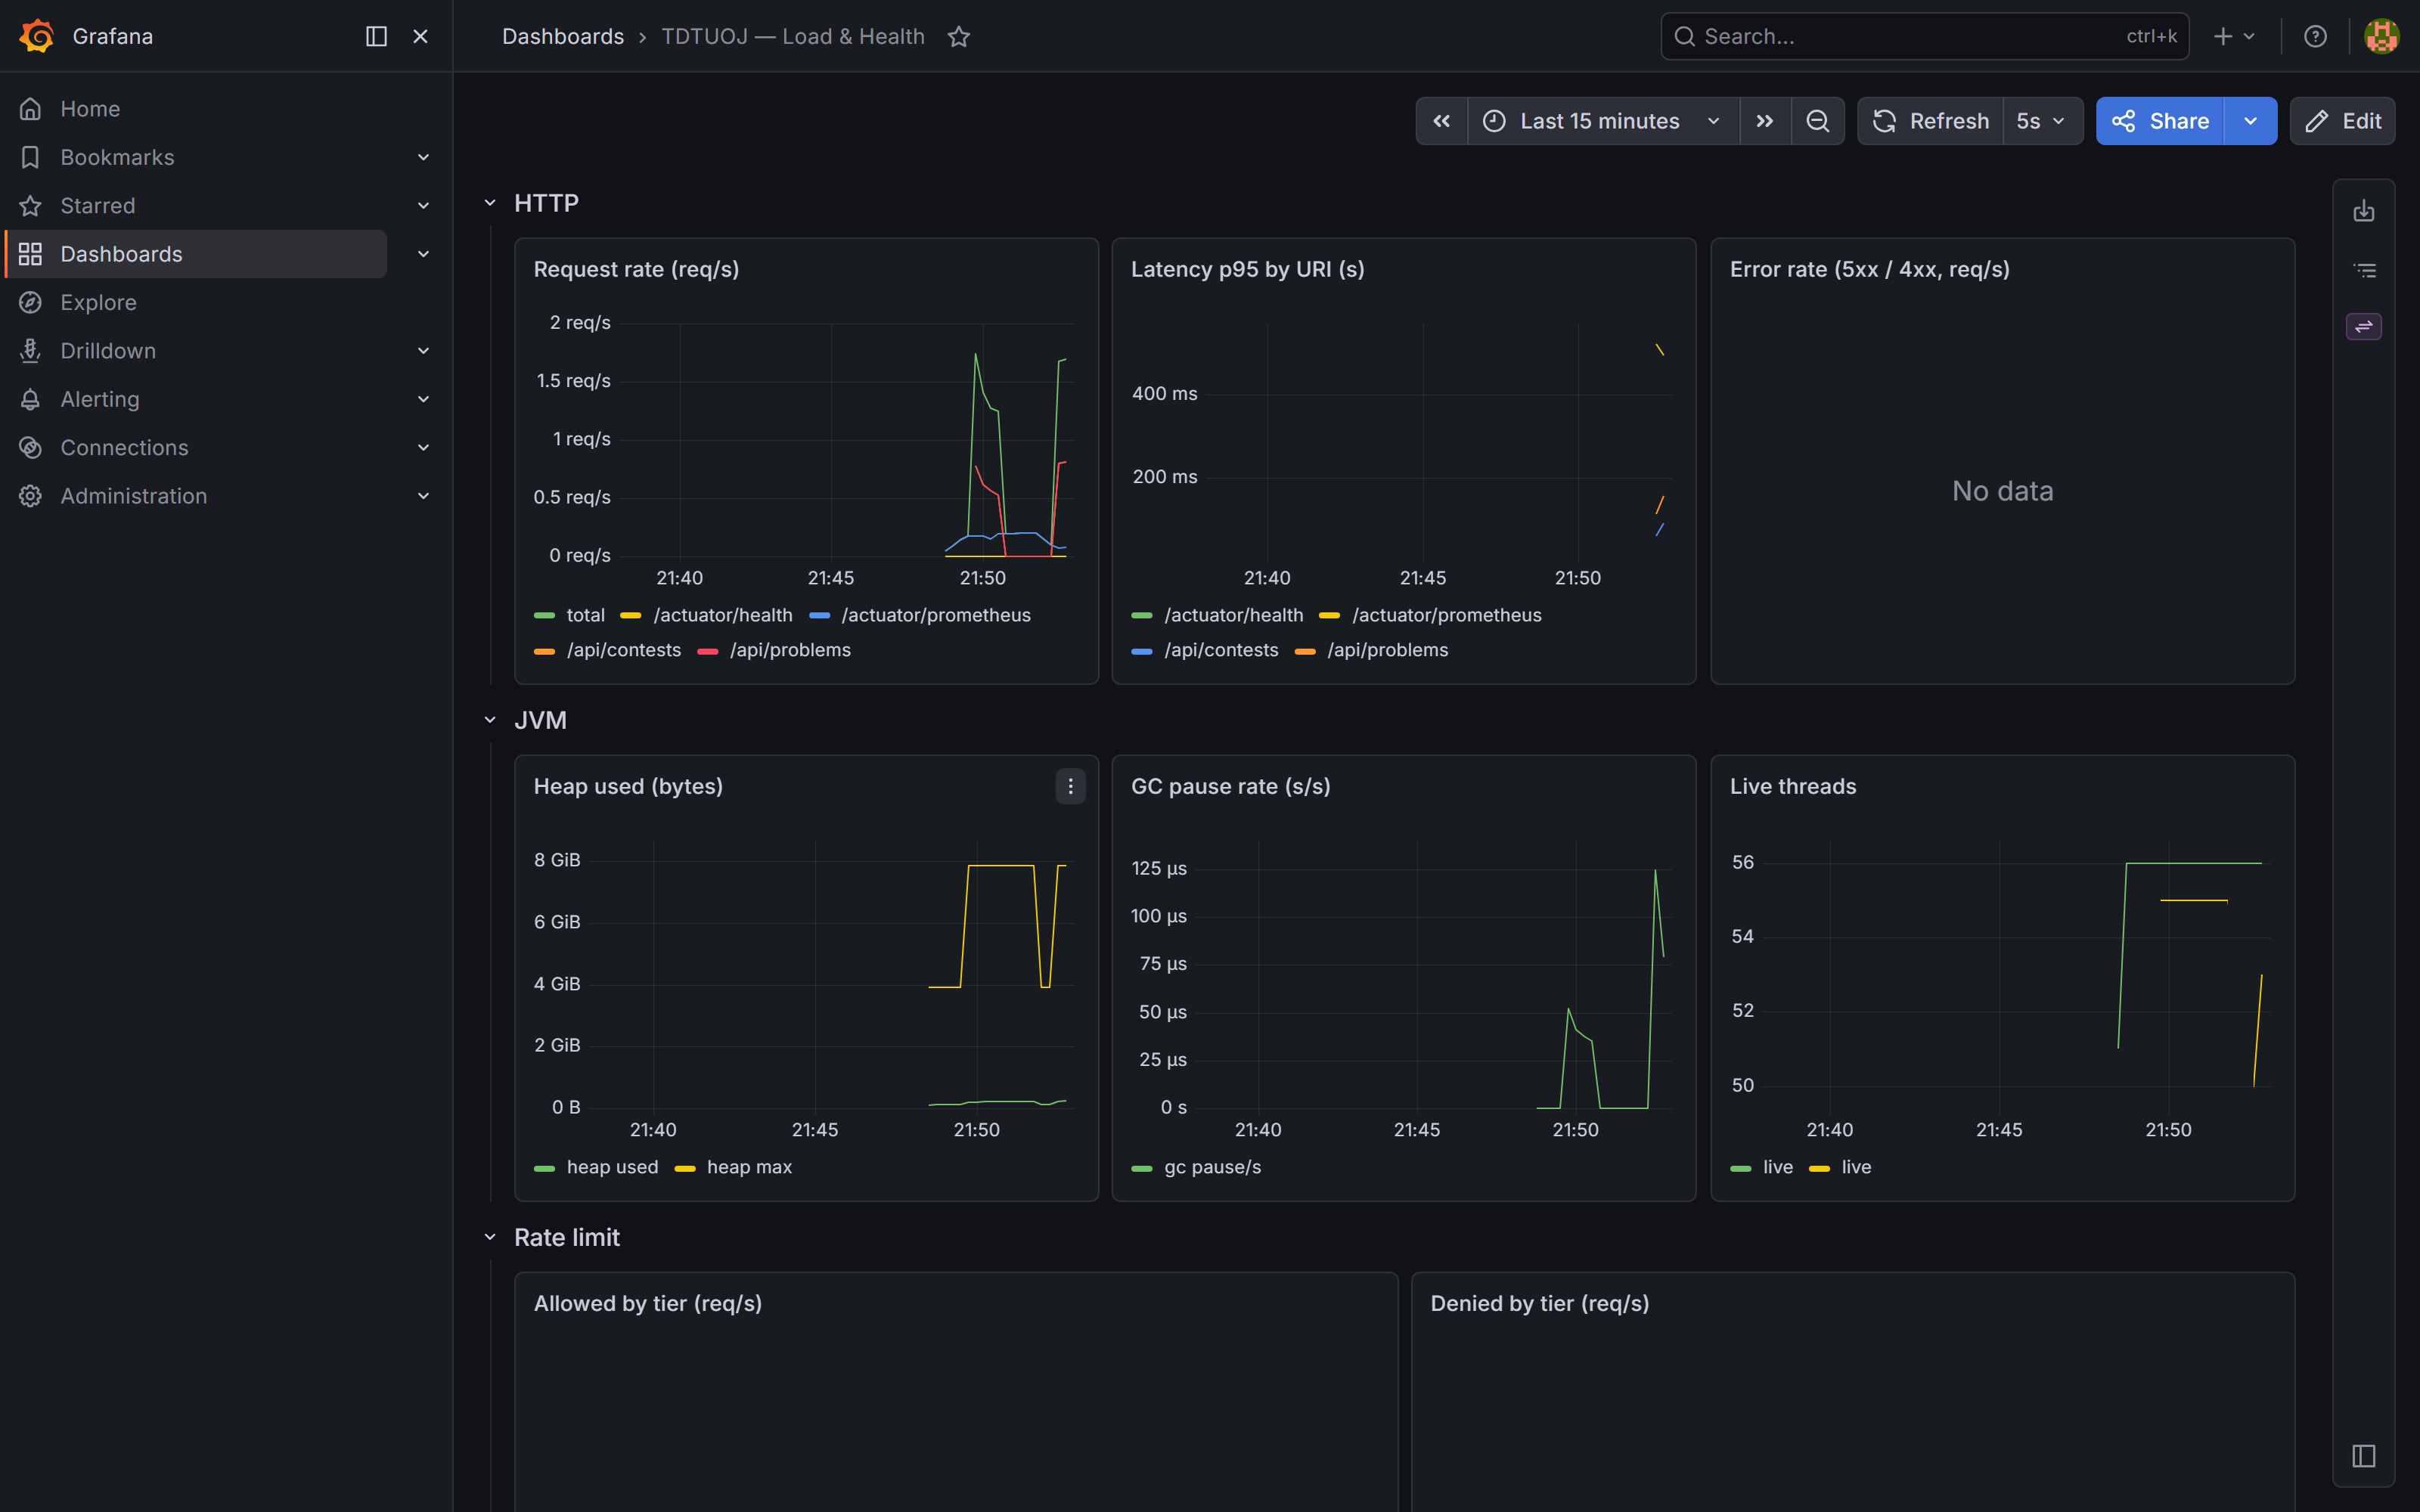
\includegraphics[width=\textwidth]{figures/grafana-dashboard.png}
  \caption{Bảng điều khiển giám sát tổng quan trên Grafana}\label{fig:grafana-dashboard}
\end{figure}

Các chỉ số được theo dõi thuộc ba lớp: lớp giao thức \ac{HTTP}, lớp máy ảo Java (\ac{JVM})
và lớp nghiệp vụ. Bảng~\ref{tab:metrics} mô tả ý nghĩa của các chỉ số chính.

\begin{table}[H]
  \centering
  \begin{tabular}{|>{\raggedright\arraybackslash}p{5.5cm}|>{\raggedright\arraybackslash}p{5.5cm}|>{\raggedright\arraybackslash}p{2cm}|}
    \hline
    \multicolumn{1}{|c|}{\textbf{Chỉ số}}
      & \multicolumn{1}{c|}{\textbf{Ý nghĩa}}
      & \multicolumn{1}{c|}{\textbf{Lớp}} \\
    \hline
    Số request mỗi giây & Thông lượng phía máy chủ phục vụ được & \ac{HTTP} \\
    \hline
    Độ trễ phân vị 95 & Thời gian phản hồi của 95\% số request & \ac{HTTP} \\
    \hline
    Bộ nhớ heap, thời gian dọn rác & Áp lực tài nguyên bộ nhớ & \ac{JVM} \\
    \hline
    Độ sâu hàng đợi chấm bài & Số bài nộp đang chờ chấm & Nghiệp vụ \\
    \hline
    Thông lượng chấm bài theo kết quả & Số bài chấm xong mỗi giây theo kết quả
      & Nghiệp vụ \\
    \hline
    Số lượt chấp nhận, từ chối theo tầng & Hiệu quả của cơ chế giới hạn tần suất
      & Nghiệp vụ \\
    \hline
  \end{tabular}
  \caption{Các chỉ số giám sát chính}\label{tab:metrics}
\end{table}

\subsection{Môi trường kiểm thử}

Toàn bộ quá trình kiểm thử được thực hiện trên một máy tính cá nhân với bộ xử lý 10 nhân
và 16 gigabyte bộ nhớ. Máy chủ ứng dụng, Judge0, công cụ sinh tải k6, Prometheus và Grafana
đều chạy đồng thời trên cùng máy này và chia sẻ chung tài nguyên phần cứng. Do đó, các số
liệu thu được mang tính so sánh tương đối, phản ánh xu hướng và hành vi của hệ thống dưới
tải, thay vì năng lực tuyệt đối trong môi trường triển khai thực tế.

\subsection{Các kịch bản kiểm thử}

Quá trình kiểm thử tải sử dụng ba kịch bản, mỗi kịch bản tập trung vào một khía cạnh khác
nhau của hệ thống.

Kịch bản thứ nhất mô phỏng việc duyệt nội dung với số người dùng ảo tăng dần. Cụ thể, số
người dùng ảo tăng từ 0 lên 100 trong vòng một phút, duy trì ở mức đó trong hai phút, rồi
giảm về 0 trong 30 giây. Mỗi người dùng ảo lần lượt truy vấn danh sách bài toán, trang chi
tiết một bài toán và danh sách cuộc thi. Ngưỡng chấp nhận được đặt ở tỉ lệ lỗi dưới 5\%
và độ trễ phân vị 95 dưới một giây.

Kịch bản thứ hai mô phỏng nộp bài liên tục để quan sát hoạt động của hàng đợi và tiến trình
chấm bài. Tốc độ nộp bài tăng dần từ 1 lên 20 bài mỗi giây trong 30 giây, duy trì ở mức
đỉnh trong một phút, rồi giảm về 0 trong 30 giây. Kịch bản sử dụng tối đa 200 người dùng ảo
và theo dõi độ sâu hàng đợi cùng thông lượng chấm bài qua Grafana.

Kịch bản thứ ba dồn dập gửi request vượt ngưỡng cho phép nhằm kiểm chứng cơ chế giới hạn
tần suất. Năm mươi người dùng ảo liên tục gửi request đến endpoint đăng nhập trong 90 giây
với thông tin đăng nhập không hợp lệ, qua đó chỉ kích hoạt bộ đếm tần suất truy cập mà không tạo
phiên đăng nhập hợp lệ.

\subsection{Kết quả kiểm thử}

Trong kịch bản giới hạn tần suất, kết quả đo cho thấy số lượt request được chấp nhận duy trì
ở mức trần đã cấu hình, trong khi số lượt bị từ chối tăng vọt khi lưu lượng vượt ngưỡng, như
minh họa ở Hình~\ref{fig:grafana-ratelimit}. Điều này xác nhận cơ chế bảo vệ hoạt động đúng
khi hệ thống bị truy cập dồn dập.

\begin{figure}[H]
  \centering
  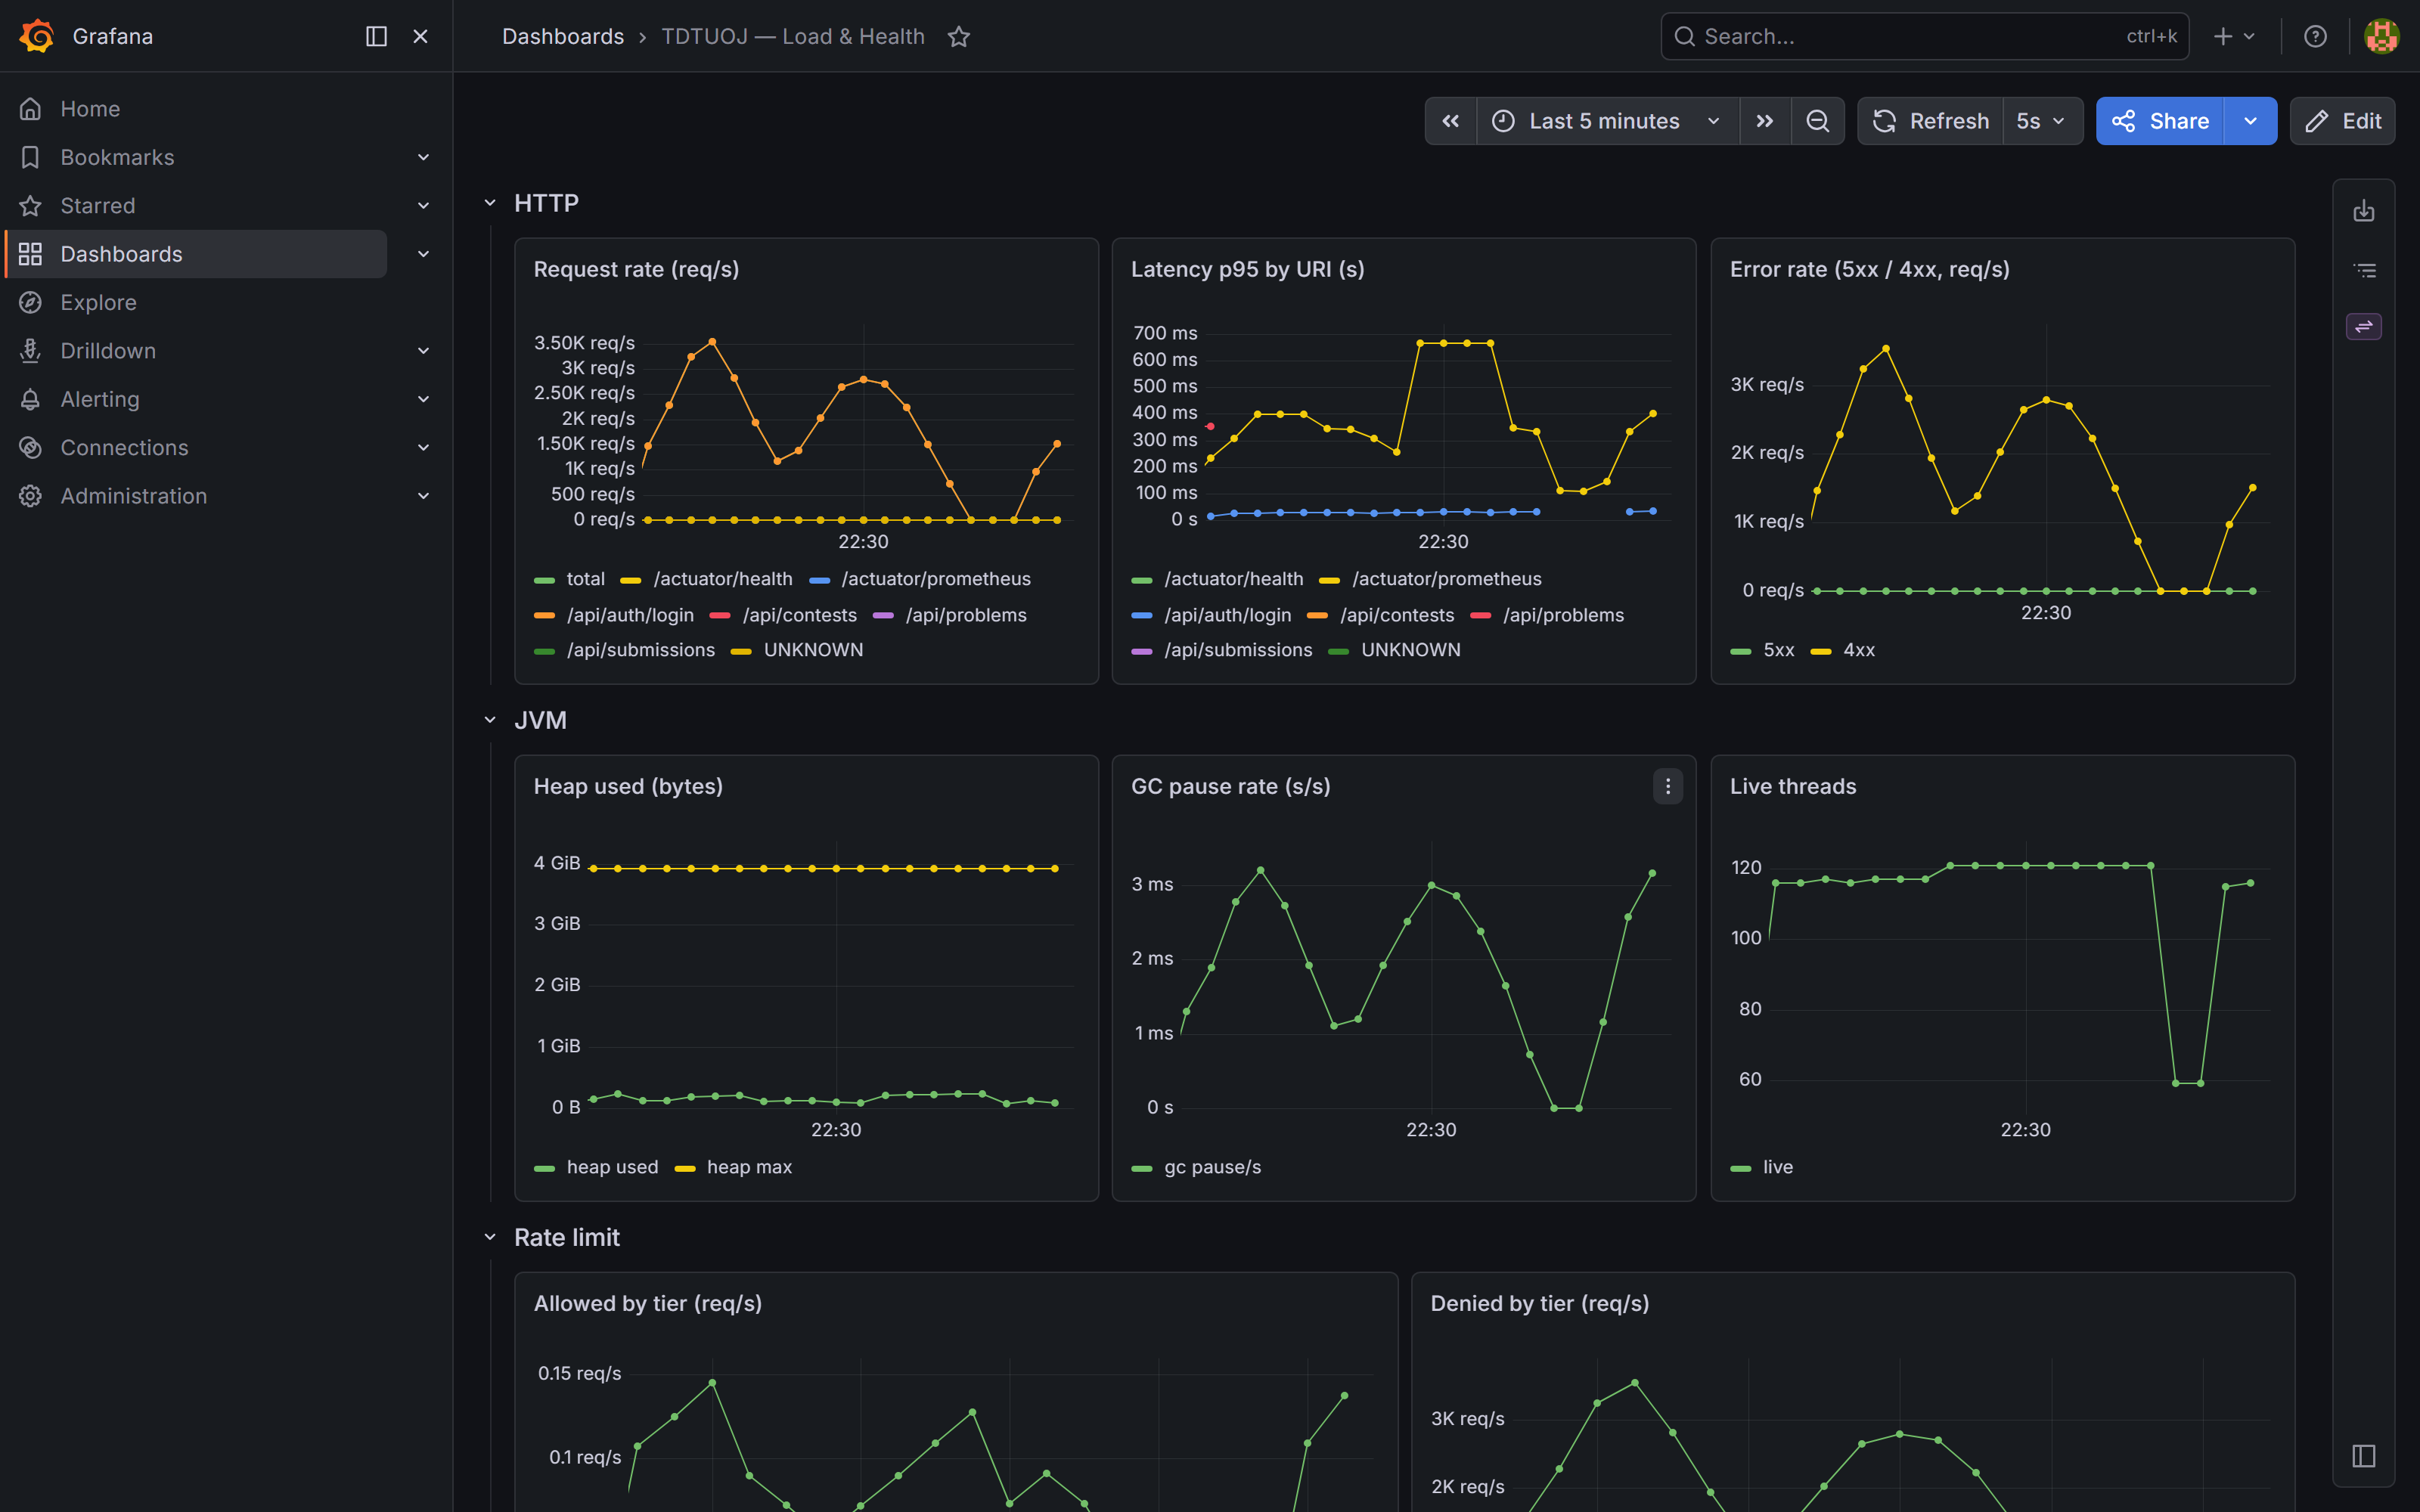
\includegraphics[width=\textwidth]{figures/grafana-ratelimit.png}
  \caption{Số lượt chấp nhận và từ chối theo tầng khi bị dồn tần suất}\label{fig:grafana-ratelimit}
\end{figure}

Trong kịch bản nộp bài, hàng đợi chấm bài tích lũy khi tải tăng rồi thoát dần ổn định khi
tốc độ nộp giảm, không xảy ra tình trạng nghẽn kéo dài. Lưu lượng \ac{HTTP} và mức tiêu thụ
tài nguyên \ac{JVM} đều ổn định trong suốt quá trình, như trình bày ở
Hình~\ref{fig:grafana-submit}.

\begin{figure}[H]
  \centering
  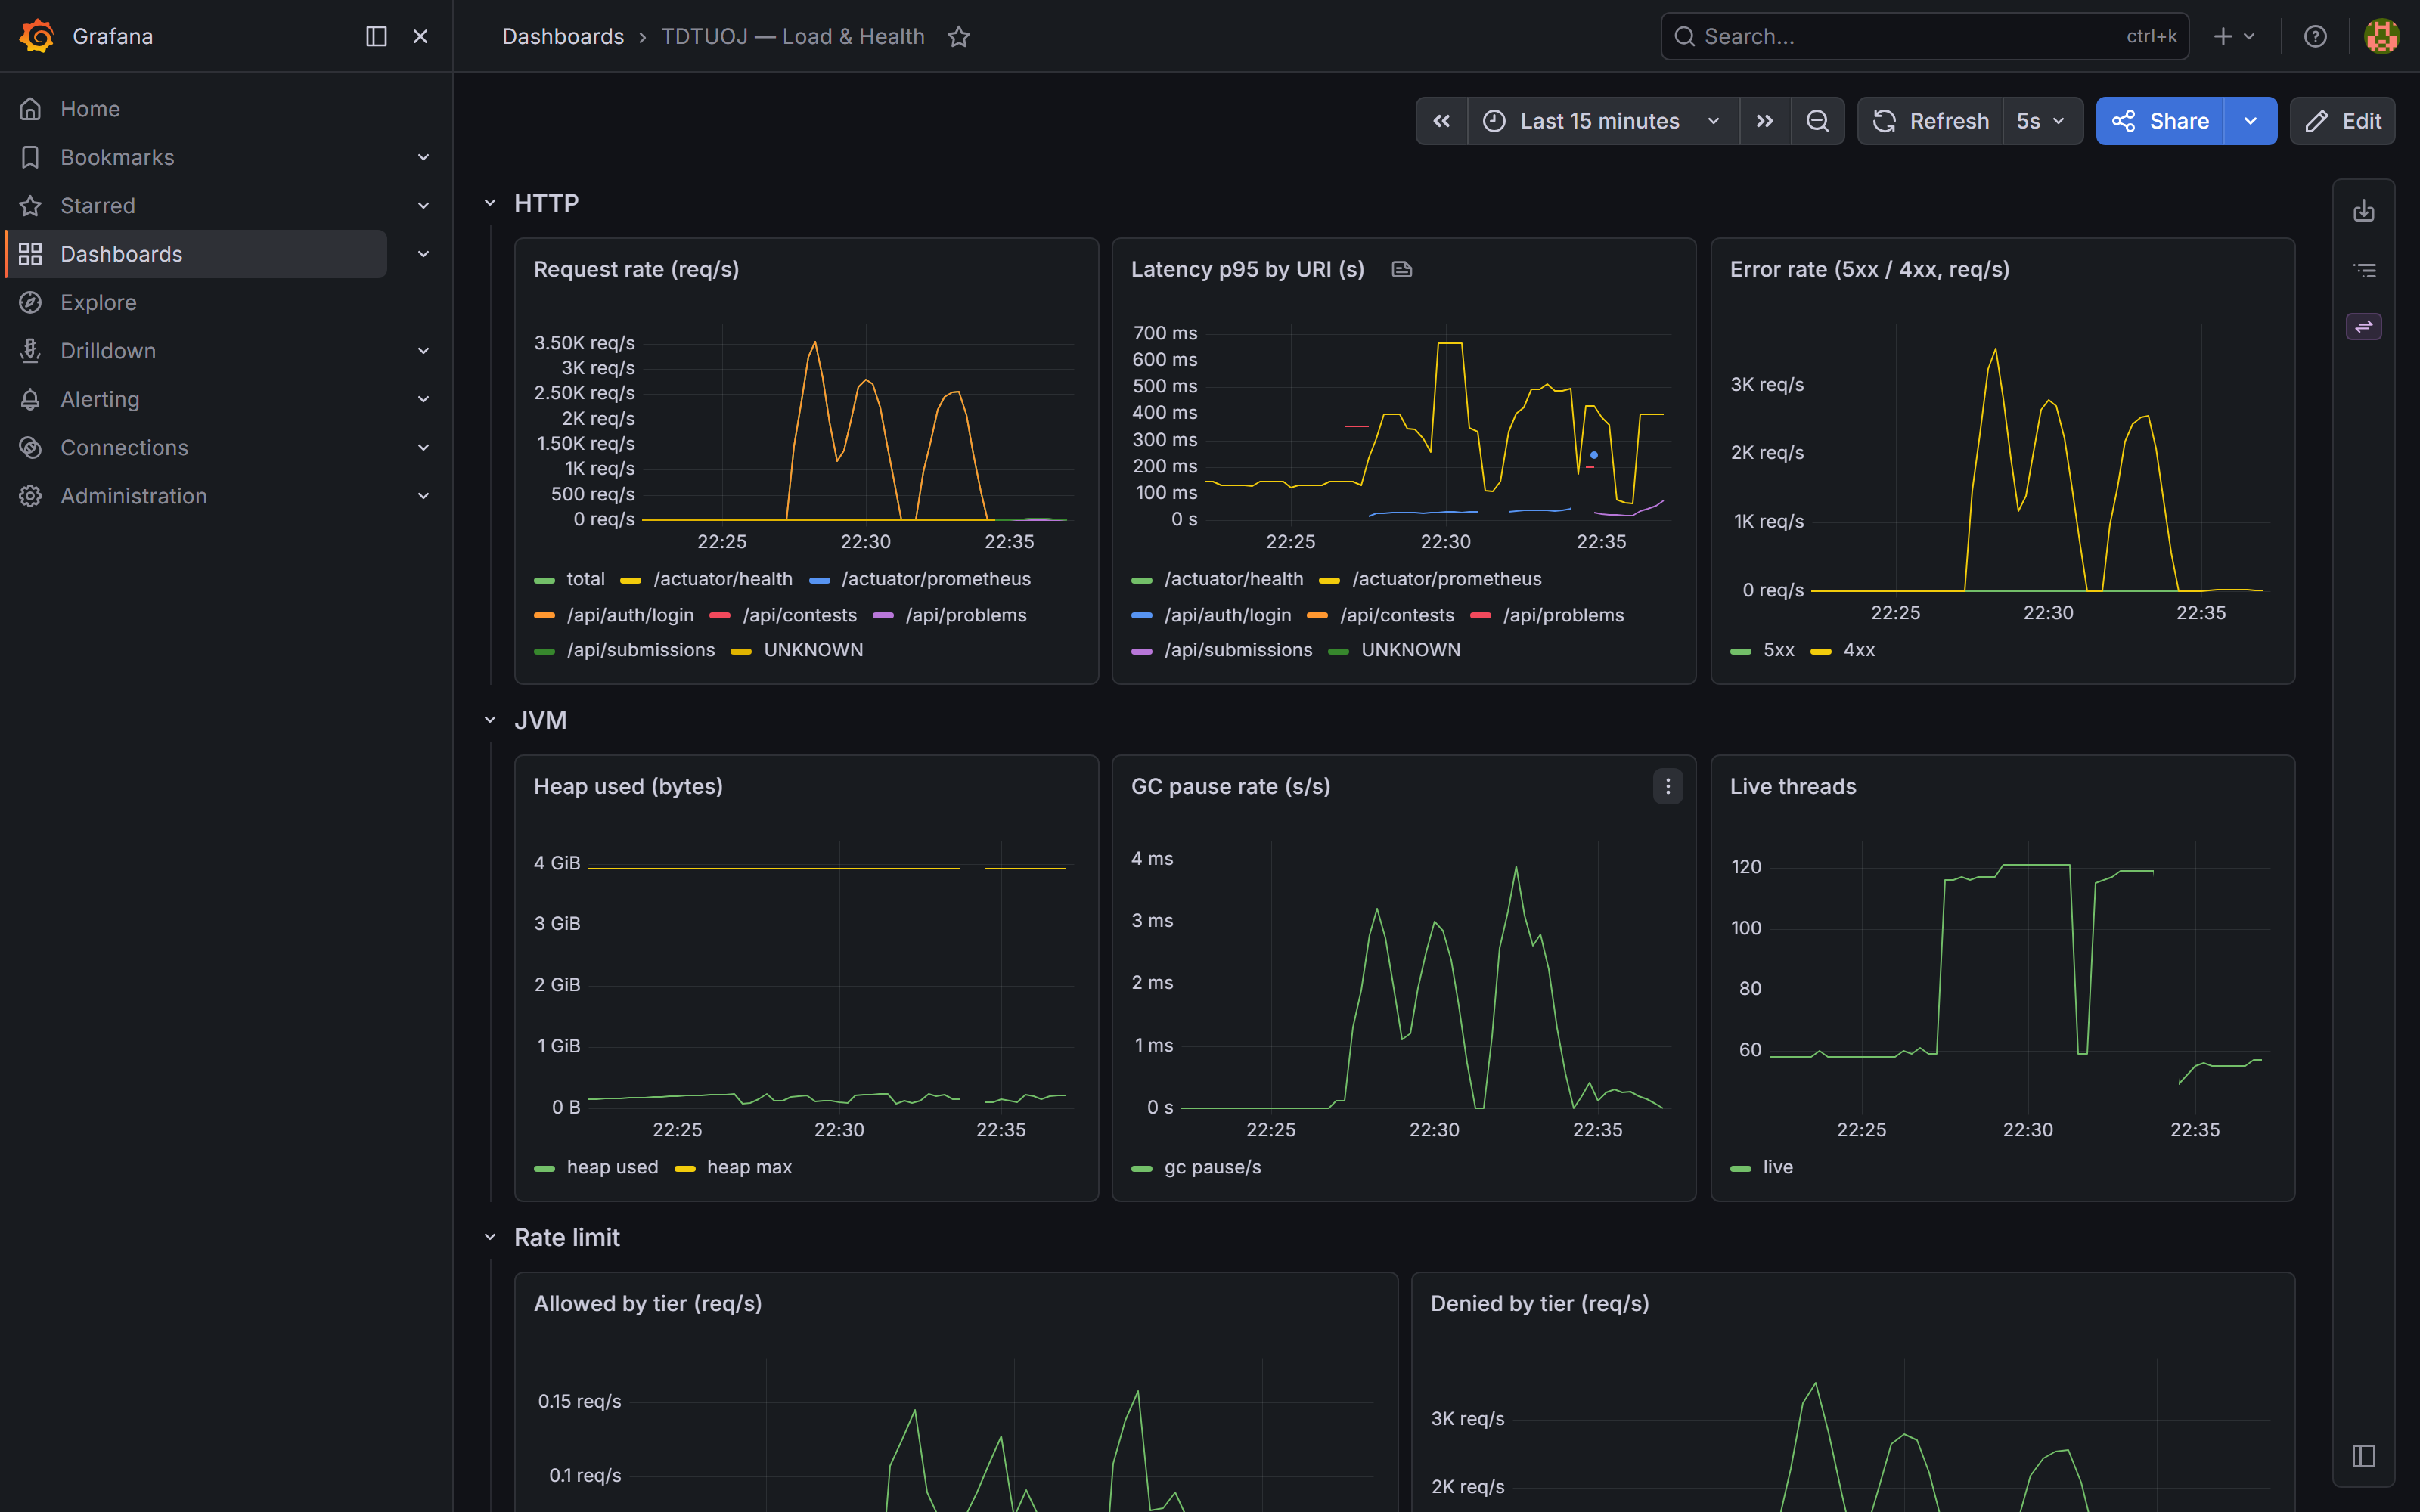
\includegraphics[width=\textwidth]{figures/grafana-submit.png}
  \caption{Giám sát hệ thống trong kịch bản nộp bài}\label{fig:grafana-submit}
\end{figure}

Nhìn chung, kết quả kiểm thử tải cho thấy hệ thống đáp ứng ổn định dưới lưu lượng cao,
tỉ lệ lỗi và độ trễ nằm trong ngưỡng chấp nhận, và cơ chế giới hạn tần suất bảo vệ hiệu
quả khi bị tấn công dồn dập.

% ============================================================
% CHƯƠNG 6 – TRIỂN KHAI HỆ THỐNG
% ============================================================
\chapter{Triển khai hệ thống}

Sau khi hoàn thiện và kiểm thử, hệ thống TDTUOJ được triển khai lên môi trường trực tuyến
nhằm phục vụ việc sử dụng thực tế. Chương này trình bày hạ tầng và công cụ
được sử dụng để triển khai, quy trình đưa hệ thống lên môi trường vận hành kèm cơ chế tích
hợp và triển khai liên tục (\ac{CI/CD}), cùng kết quả đạt được và chi phí vận hành hằng
tháng.

\section{Hạ tầng và công cụ triển khai}

Toàn bộ phần phía máy chủ được triển khai theo mô hình đóng gói bằng vùng chứa (container).
Mã nguồn phía máy chủ được biên dịch thành một image Docker, sau đó toàn bộ các thành phần
phụ thuộc được khai báo và khởi chạy đồng thời trên cùng một máy ảo thông qua
công cụ Docker Compose. Cách làm này bảo đảm môi trường vận hành nhất quán với môi trường
phát triển và có thể tái dựng lại toàn bộ hệ thống chỉ bằng một câu lệnh.

Máy ảo được thuê từ dịch vụ điện toán đám mây Microsoft Azure, theo gói dành cho sinh viên
(Azure for Students), với cấu hình hai nhân xử lý, tám gigabyte bộ nhớ và hệ điều hành Ubuntu.
Trên máy ảo này, Docker Compose điều phối tám vùng chứa chạy đồng thời: phía máy chủ Spring
Boot; cơ sở dữ liệu PostgreSQL và bộ nhớ đệm Redis của ứng dụng; cụm dịch vụ chấm bài Judge0
cùng cơ sở dữ liệu và bộ nhớ đệm riêng của nó; và một máy chủ ủy nhiệm ngược (reverse proxy)
Caddy. Trong đó, Caddy đóng vai trò cổng vào duy nhất: nó tự động xin và gia hạn chứng chỉ số
để cung cấp kết nối mã hóa \ac{HTTPS} qua giao thức \ac{TLS}, đồng thời chuyển tiếp request đến
phía máy chủ. Các thành phần còn lại chỉ giao tiếp nội bộ trong mạng riêng của Docker Compose,
không mở trực tiếp ra Internet.

Phía giao diện người dùng được triển khai tách biệt trên nền tảng Vercel. Nền tảng này chuyên
dùng cho các ứng dụng web tĩnh; nó tự động biên dịch và phân phối mã nguồn React qua mạng phân
phối nội dung toàn cầu. Hệ thống dùng tên miền riêng tdtuoj.me: tên miền gốc trỏ tới giao diện
trên Vercel, còn tên miền phụ api.tdtuoj.me trỏ tới phía máy chủ trên máy ảo; việc phân giải
được cấu hình qua các bản ghi \ac{DNS}. Tên miền này được đăng ký qua nhà cung cấp Namecheap và
miễn phí năm đầu nhờ gói ưu đãi GitHub Student Developer Pack dành cho sinh viên. Cả hai đầu đều
được bảo vệ bằng \ac{HTTPS}, nhờ đó cơ chế đăng nhập bằng tài khoản Google hoạt động đúng yêu
cầu bảo mật. Bảng~\ref{tab:deploy-stack}
tổng hợp các thành phần hạ tầng chính.

\begin{table}[H]
  \centering
  \begin{tabular}{|>{\raggedright\arraybackslash}p{4cm}|>{\raggedright\arraybackslash}p{4.5cm}|>{\raggedright\arraybackslash}p{4.5cm}|}
    \hline
    \multicolumn{1}{|c|}{\textbf{Thành phần}}
      & \multicolumn{1}{c|}{\textbf{Công cụ / dịch vụ}}
      & \multicolumn{1}{c|}{\textbf{Vai trò}} \\
    \hline
    Phía máy chủ + chấm bài & Máy ảo Azure (Docker Compose) & Chạy backend, Judge0,
      cơ sở dữ liệu, bộ nhớ đệm \\
    \hline
    Cổng vào \& \ac{HTTPS} & Caddy & Ủy nhiệm ngược, tự cấp chứng chỉ \ac{TLS} \\
    \hline
    Phía giao diện & Vercel & Phân phối ứng dụng React \\
    \hline
    Tên miền \& phân giải & Namecheap (\ac{DNS}) & Tên miền tdtuoj.me \\
    \hline
    Tích hợp liên tục & GitHub Actions & Tự động biên dịch và triển khai \\
    \hline
  \end{tabular}
  \caption{Các thành phần hạ tầng triển khai chính}\label{tab:deploy-stack}
\end{table}

\section{Quy trình triển khai và tích hợp liên tục}

Quy trình đưa hệ thống lên môi trường vận hành gồm nhiều bước. Trước hết, máy ảo được khởi tạo
và mở các cổng cần thiết, sau đó cài đặt Docker và sao chép mã nguồn về máy. Tiếp theo, các
thông tin bí mật như mật khẩu cơ sở dữ liệu, khóa bí mật và khóa truy cập dịch vụ ngoài được
khai báo trong một tập tin cấu hình riêng, không đưa vào kho mã nguồn. Cuối cùng, toàn bộ hệ
thống được khởi chạy bằng Docker Compose. Song song đó, việc cấu hình các bản ghi \ac{DNS} và
để Caddy tự cấp chứng chỉ giúp hoàn tất kết nối \ac{HTTPS}.

Để giảm thao tác thủ công mỗi khi cập nhật mã nguồn, đề tài thiết lập một quy trình \ac{CI/CD}
bằng GitHub Actions. Mỗi khi mã nguồn được đẩy lên nhánh chính, hệ thống tự động chạy hai giai
đoạn. Giai đoạn đầu kiểm tra biên dịch và chạy các trường hợp kiểm thử đơn vị để bảo đảm mã
nguồn hợp lệ. Nếu bước này thành công, giai đoạn sau kết nối tới máy ảo qua giao thức \ac{SSH},
cập nhật mã nguồn mới và dựng lại các vùng chứa. Riêng phía giao diện trên Vercel được tự động
biên dịch và phân phối lại ngay khi có thay đổi, không cần cấu hình thêm. Nhờ vậy, mỗi thay đổi
trong mã nguồn đều được đưa lên môi trường vận hành một cách tự động và nhất quán.

\section{Kết quả triển khai và chi phí vận hành}

Hệ thống đã được triển khai thành công và truy cập được công khai tại địa chỉ
https://tdtuoj.me, với phía máy chủ phục vụ tại https://api.tdtuoj.me. Các
chức năng chính đều hoạt động đúng trong môi trường vận hành thực tế: người dùng đăng ký và
đăng nhập (kể cả đăng nhập bằng tài khoản Google), duyệt và nộp bài, dịch vụ Judge0 chấm bài
và trả kết quả chính xác, kết nối được mã hóa \ac{HTTPS} đầu cuối. Quy trình \ac{CI/CD} cũng
vận hành đúng, tự động cập nhật hệ thống sau mỗi lần thay đổi mã nguồn.

Về chi phí, hầu hết các dịch vụ đều thuộc các gói miễn phí dành cho sinh viên hoặc nhà phát
triển. Khoản chi phí đáng kể duy nhất là máy ảo trên Azure. Với cấu hình đã chọn, đơn giá
xấp xỉ 62 đô-la Mỹ mỗi tháng nếu để chạy liên tục cả ngày lẫn đêm. Tuy
nhiên, Azure chỉ tính phí phần xử lý theo số giờ máy ảo thực sự hoạt động; khi không cần
sử dụng, máy ảo được giải phóng tài nguyên (deallocate) nên phần phí xử lý trở về không,
chỉ còn phí lưu trữ đĩa và địa chỉ mạng tĩnh ở mức thấp, khoảng 5 đến 9
đô-la Mỹ mỗi tháng.

\begin{table}[H]
  \centering
  \begin{tabular}{|>{\raggedright\arraybackslash}p{4.5cm}|>{\raggedright\arraybackslash}p{8cm}|}
    \hline
    \multicolumn{1}{|c|}{\textbf{Thành phần}}
      & \multicolumn{1}{c|}{\textbf{Chi phí hằng tháng}} \\
    \hline
    Máy ảo Azure (đang chạy) & Khoảng 62 đô-la Mỹ nếu chạy liên tục 24/7 \\
    \hline
    Máy ảo Azure (đã giải phóng) & Khoảng 5 đến 9 đô-la Mỹ (chỉ phí đĩa và địa chỉ mạng tĩnh) \\
    \hline
    Phía giao diện (Vercel) & Miễn phí (gói Hobby) \\
    \hline
    Tên miền tdtuoj.me (Namecheap) & Miễn phí năm đầu qua GitHub Student, khoảng 20 đô-la Mỹ mỗi năm sau đó \\
    \hline
    Tích hợp liên tục (GitHub Actions) & Miễn phí \\
    \hline
  \end{tabular}
  \caption{Chi phí vận hành các thành phần triển khai}\label{tab:deploy-cost}
\end{table}

Nhìn chung, việc triển khai cho thấy hệ thống TDTUOJ không chỉ hoạt động được trong môi
trường phát triển mà còn vận hành ổn định trên môi trường trực tuyến thực tế với chi phí
hợp lý, đồng thời có thể tái dựng nhanh chóng nhờ mô hình đóng gói bằng vùng chứa.

% ============================================================
% CHƯƠNG 7 – KẾT LUẬN
% ============================================================
\chapter{Kết luận}

\section{Kết quả đạt được}

Đề tài đã xây dựng hoàn chỉnh hệ thống chấm bài trực tuyến TDTUOJ phục vụ việc giảng dạy
và rèn luyện lập trình tại Khoa Công nghệ Thông tin, Trường Đại học Tôn Đức Thắng. Hệ
thống bao phủ trọn vẹn luồng nghiệp vụ của một nền tảng chấm bài: quản lý kho bài toán với
phân quyền công khai/riêng tư, nộp bài và chấm tự động bất đồng bộ qua Judge0 với bốn
ngôn ngữ lập trình, tổ chức cuộc thi theo thể thức \ac{ICPC} kèm bảng xếp hạng
thời gian thực, cơ chế đóng băng bảng xếp hạng và tính điểm đánh giá năng lực sau cuộc
thi, cùng mô hình tổ chức/bài thực hành phục vụ quản lý lớp học của giảng viên.

Bên cạnh các chức năng cốt lõi, đề tài đóng góp hai nhóm tính năng hỗ trợ học tập có tính
đặc thù. Thứ nhất là trình trực quan hóa cấu trúc dữ liệu: mã nguồn của người dùng được
biến đổi để tự ghi vết khi thực thi, kết hợp mô hình ngôn ngữ lớn phân loại vai trò ngữ
nghĩa của biến, cho phép minh họa từng bước chạy của thuật toán trên sáu ngôn ngữ lập
trình. Thứ hai là lớp hỗ trợ học tập bằng \ac{LLM}: gợi ý hướng giải có kiểm soát không
tiết lộ lời giải, trích xuất đề bài tự động từ tập tin \ac{PDF} và sinh trường hợp kiểm
thử, giúp giảm đáng kể công sức soạn đề của giảng viên.

Về mặt kỹ thuật, hệ thống được thiết kế theo kiến trúc phân tầng với xác thực phi trạng
thái bằng \ac{JWT}, hàng đợi chấm bài và bộ nhớ đệm trên Redis, giới hạn tần suất truy cập
theo thuật toán token bucket, cùng hạ tầng giám sát bằng Prometheus và Grafana. Chất lượng
được kiểm chứng qua 101 trường hợp kiểm thử đơn vị cho tầng nghiệp vụ và các kịch bản kiểm thử tải
xác nhận hệ thống vận hành ổn định dưới lưu lượng cao.

Ngoài ra, hệ thống đã được triển khai thành công lên môi trường trực tuyến thực tế và truy
cập được công khai qua tên miền riêng với kết nối mã hóa \ac{HTTPS}. Toàn bộ phần phía máy
chủ được đóng gói bằng vùng chứa và điều phối bằng Docker Compose trên một máy ảo đám mây,
phía giao diện được phân phối trên Vercel, kèm quy trình tích hợp và triển khai liên tục
(\ac{CI/CD}) tự động cập nhật hệ thống sau mỗi thay đổi mã nguồn. Việc triển khai chứng tỏ
hệ thống có thể vận hành thực tế với chi phí hợp lý nhờ tận dụng các gói dịch vụ miễn phí
dành cho sinh viên.

\section{Hạn chế}

Bên cạnh các kết quả đạt được, hệ thống còn một số hạn chế. Thứ nhất, các phép đo hiệu
năng được thực hiện trên một máy tính cá nhân nơi mọi thành phần chia sẻ tài nguyên, nên
chưa phản ánh năng lực thực tế trong môi trường triển khai phân tán. Thứ hai, độ phủ kiểm
thử đơn vị mới tập trung ở các phân hệ nghiệp vụ cốt lõi, các thành phần ngoại vi như tầng
điều khiển và trình minh họa chưa được kiểm thử ở mức đơn vị. Thứ ba, kết quả chấm bài
được phía giao diện truy vấn định kỳ (polling) thay vì đẩy chủ động, gây độ trễ nhỏ và
lưu lượng dư thừa khi nhiều người cùng chờ kết quả. Cuối cùng, các tính năng phụ thuộc
\ac{LLM} chịu ràng buộc về chi phí và hạn mức gọi dịch vụ bên ngoài, đồng thời chất lượng
phản hồi chưa thể bảo đảm tuyệt đối trong mọi tình huống.

\section{Hướng phát triển}

Trong thời gian tới, hệ thống có thể được phát triển theo một số hướng. Trước hết, từ nền
tảng đã được triển khai trực tuyến trên một máy ảo đám mây, có thể tách các thành phần ra
nhiều máy chủ riêng biệt, đặc biệt là cụm dịch vụ chấm bài, nhằm nâng cao khả năng chịu tải
và đánh giá lại hiệu năng trong điều kiện phân tán thực tế. Về chức năng, các
hướng mở rộng gồm: thay cơ chế truy vấn định kỳ bằng kết nối WebSocket để đẩy kết quả chấm
theo thời gian thực; bổ sung ngôn ngữ lập trình mới vốn đã được Judge0 hỗ trợ sẵn; xây
dựng cơ chế phát hiện đạo văn mã nguồn giữa các bài nộp trong cuộc thi; và tích hợp với
hệ thống quản lý học tập của khoa để đồng bộ danh sách lớp và điểm số. Về chất
lượng, việc mở rộng độ phủ kiểm thử sang tầng điều khiển và bổ sung kiểm thử tích hợp tự
động sẽ giúp hệ thống sẵn sàng hơn cho vận hành lâu dài.

% ============================================================
% TÀI LIỆU THAM KHẢO
% ============================================================
\newpage
\nocite{*}
\printbibliography[
  title   = {TÀI LIỆU THAM KHẢO},
  heading = bibintoc,
]

\end{document}